\documentclass[uplatex, dvipdfmx]{jsreport}
\title{関数論再建}
\author{司馬博文}
\date{\today}
\pagestyle{headings} \setcounter{secnumdepth}{4}
\input{/Users/Hirofumi Shiba/NatureOfStatistics/preamble_no_fonts.tex}
%\input{/Users/hirofumi.shiba48/NatureOfStatistics/preamble_no_fonts.tex}
\usepackage[math]{anttor}
\newcommand{\Logdomain}{\C\setminus(-\infty,0]}
\begin{document}
\tableofcontents

\chapter{正則関数}

\section{正則関数の定義と幾何学的性質}

\begin{tcolorbox}[colframe=ForestGreen, colback=ForestGreen!10!white,breakable,colbacktitle=ForestGreen!40!white,coltitle=black,fonttitle=\bfseries\sffamily,
title=]
    のちに等角写像として特徴付けるが,それ以前にそのことを匂わせる幾何学的性質を豊かに持つ.
\end{tcolorbox}

\subsection{定義と調和関数との関係}

\begin{tcolorbox}[colframe=ForestGreen, colback=ForestGreen!10!white,breakable,colbacktitle=ForestGreen!40!white,coltitle=black,fonttitle=\bfseries\sffamily,
title=]
    正則関数に対する命題は,共役な調和関数の組に関する命題に他ならない.
    より精密な議論は,調和関数を平均値の性質を持つ実関数として特徴付ける必要がある.
\end{tcolorbox}

\begin{definition}[regular / analytic function]
    関数$f:\C\osup D\to\C$が各点において微分係数を持つとき,\textbf{正則}または\textbf{解析的}という.
\end{definition}

\begin{lemma}[正則関数が定める実関数・共役調和関数が定める正則関数]
    $f:D\to\C$を正則関数とする.$f=u+iv$と表せるとき,$u,v:D\to\R$を\textbf{実部}と\textbf{虚部}という.これらは,
    \begin{enumerate}
        \item Cauchy-Riemann方程式を満たす:$u_x=v_y,u_y=-v_x$.
        \item 調和関数である:$\Laplace u=0,\Laplace v=0$.
    \end{enumerate}
    一般に,上の2条件を満たす実関数の組$(u,v)$を\textbf{共役調和関数}という.次が成り立つ:
    \begin{enumerate}\setcounter{enumi}{2}
        \item $u,v$を共役調和関数とする.$u+iv$は正則関数である.
    \end{enumerate}
\end{lemma}

\begin{definition}
    実関数$u\in C^2(D;\R)$が\textbf{調和関数}または\textbf{ポテンシャル関数}であるとは,$\Laplace u=0$を満たすことをいう.
\end{definition}

\begin{proposition}[調和関数が定める正則関数]
    $u$を調和関数とする.$\pp{u}{x}+\frac{1}{i}\pp{u}{v}$は正則関数である.
\end{proposition}

\begin{proposition}[Hodge duality]
    $u\in C^2(D;\R)$を調和関数とし,$f:=u_x-iu_y$を付随する正則関数とする.
    このとき,$u$の共役調和関数$v$(存在するとは限らない)の微分に当たるものを${}^*du:=-\pp{u}{y}dx+\pp{u}{x}dy\paren{=\pp{v}{x}dx+\pp{v}{y}dy}$とおくと,
    $fdz=du+i{}^*du$と表せる.
\end{proposition}
\begin{remarks}
    Hodge双対の積分は,右法線微分の積分とみなせる.
\end{remarks}

\subsection{Cauchy-Riemann作用素による特徴付け}

\begin{tcolorbox}[colframe=ForestGreen, colback=ForestGreen!10!white,breakable,colbacktitle=ForestGreen!40!white,coltitle=black,fonttitle=\bfseries\sffamily,
title=]
    複素関数$u\in C^1(D)$の微分$du$の,$d\o{z}$の係数が消えるものを,複素微分可能であるという.
\end{tcolorbox}

\begin{definition}[Wirtinger derivative / Cauchy-Riemann operator, differential of complex function]\mbox{}
    \begin{enumerate}
        \item 次によって定まる線型作用素$\O(D)\to\O(D)$
        \begin{align*}
            \partial_z&=\frac{\partial}{\partial z}:=\frac{1}{2}\left(\frac{\partial}{\partial x}\textcolor{red}{-}i\frac{\partial}{\partial y}\right)=\frac{1}{2}\paren{\pp{}{x}+\frac{1}{i}\pp{}{y}},&
            \overline{\partial}=\partial_{\overline{z}}&:=\frac{\partial}{\partial\overline{z}}=\frac{1}{2}\left(\frac{\partial}{\partial x}\textcolor{red}{+}i\frac{\partial}{\partial y}\right)=\frac{1}{2}\paren{\pp{}{x}-\frac{1}{i}\pp{}{y}}
        \end{align*}
        を\textbf{コーシー・リーマン作用素}という.ここで,$u$が正則であるとき,$\pp{u}{z}=u'$とも表す\cite{Hormander}.
        \item 関数$f:D\to\C$が\textbf{(全)微分可能}とは,実線型関数$L:D\to \C;x+yi\mapsto\al x+\beta y\;(\al,\beta\in\C)$が存在して,$f(w+z)=f(w)+L(z)+o(\abs{z})$が成り立つことをいう.
        このとき,
        \[L=df=\pp{f}{z}dz+\pp{f}{\o{z}}d\o{z}\;\in T^*_w(\C)\]
        と表せる.
    \end{enumerate}
\end{definition}

\begin{proposition}[微分作用素による特徴付け]
    $f:D\to\C$について,次は同値.
    \begin{enumerate}
        \item $f$は$a\in D$で正則.
        \item $f$は$a\in D$で微分可能かつ$f_{\o{z}}(a)=0$.
    \end{enumerate}
\end{proposition}

\begin{corollary}[正則性の遺伝]\mbox{}
    \begin{enumerate}
        \item 正則関数の複素線型結合は正則である.
        \item 正則関数の積は正則である.
        \item 正則関数の合成は正則である.
    \end{enumerate}
\end{corollary}
\begin{Proof}\mbox{}
    \begin{enumerate}
        \item C-R作用素の線形性より.
        \item 積の微分法則$d(uv)=udv+vdu$より.
        \item $dv=v'du=v'u'dz$.
    \end{enumerate}
\end{Proof}

\subsection{Jacobian}

\begin{corollary}[正則関数の微分係数の各種表現とJacobianの特徴付け]
    $f$が$z_0\in D$で正則とする.
    \begin{enumerate}
        \item 実関数への同一視を$F(x,y):=f(z)$とすると,$F:\R^2\to\C$も微分可能であり,$\det J_F(x_0,y_0)=\abs{f'(z_0)}^2$.
        \item $f'(z_0)\ne0$ならば,$f$は$z_0$の近傍で位相同型を定め,逆も$C^1$-級である.
    \end{enumerate}
\end{corollary}
\begin{Proof}\mbox{}
    \begin{enumerate}
        \item $u$が正則ならば$du=u'dz$と表せ,写像$dz\mapsto du$とは,回転と$\abs{u'}$倍との合成である.したがって,$z\mapsto u(z)$のJacobianは$\abs{u'}^2$である.
        \item 陰関数定理による.
    \end{enumerate}
\end{Proof}
\begin{remarks}[大域的な可逆性とRiemann面のアイデア]
    陰関数定理の議論の時に夢想したことがあるであろうことに,各点でJacobianが$0$でないならば,その局所的な可逆写像を繋ぎ合わせて大域的な逆射を構成できないか?ということである.
    正則関数において,この探求の行手を阻むものはただ一つで,像が重なってしまうことである.
    そこで,定義域と値域を,重なったフィルムを引き剥がすように拡張すれば,一価な単射が定まるかもしれない.
\end{remarks}

\begin{corollary}
    $\Om\osub\C$,$f\in\O(\Om),a\in\Om$について,次の2条件は同値:
    \begin{enumerate}
        \item $f'(a)\ne0$.
        \item $f$は局所双正則.
    \end{enumerate}
\end{corollary}

\subsection{等角写像としての特徴付け}

\begin{definition}[conformal mapping]
    $C^1$-級写像$f:D\to\C$が$p\in D$で\textbf{等角}であるとは,
    $f$が引き起こす$C^1$-道の対応$\gamma\mapsto f\circ\gamma$が,
    $p$での接空間の内積を保つことをいう.
\end{definition}

\begin{proposition}[等角性による特徴付け]
    $f:D\to\C$が$C^1$-級であるとする.次は同値.
    \begin{enumerate}
        \item $p\in D$で等角である.
        \item $\partial_zf(p)\ne0$かつ$\partial_{\o{z}}f(p)=0$.
    \end{enumerate}
\end{proposition}

\section{整級数}

\begin{tcolorbox}[colframe=ForestGreen, colback=ForestGreen!10!white,breakable,colbacktitle=ForestGreen!40!white,coltitle=black,fonttitle=\bfseries\sffamily,
title=]
    正則関数を構成する強力な手法となる.特に,理論展開の初期段階で指数関数を定義するのに用いられる.
    この手法の\textbf{普遍性},すなわち任意の正則関数が整級数展開によって得られることはのちの理論で得られる.
\end{tcolorbox}

\begin{definition}
    級数のうち,$\{a_n\}\subset\C$を用いて
    $\sum_{n=0}^\infty a_nz^n$と表せるものを\textbf{整級数}という.
\end{definition}

\subsection{Abelの定理}

\begin{lemma}[整級数の収束半径の特徴付け]\label{lemma-Abel}
    \[R=\frac{1}{\limsup_{n\to\infty}\abs{a_n}^{1/n}}=\sup\Brace{r\in\R_+\mid \{\abs{a_n}r^n\}\text{は有界}}\]
\end{lemma}

\begin{theorem}[Abel]
    任意の整級数に対して,\textbf{収束半径}$R\in[0,\infty]$が定まる:
    \begin{enumerate}
        \item $\Delta(0,R)$上にて,整級数は絶対収束する.
        \item $\forall_{r\in[0,R)}$について$[\Delta(0,r)]$上にて,整級数は一様収束する.
        \item $\Delta(\infty,R)$上にて,級数は発散する.
        \item $\Delta(0,R)$上にて整級数は微分可能で,その導関数は項別微分によって得られ,同じ収束半径を持つ.特に,整関数は$\Delta(0,R)$上で正則関数を定める.
        \item 収束半径$R$は$1/R:=\limsup_{n\to\infty}\sqrt[n]{\abs{a_n}}$で与えられる.
    \end{enumerate}
\end{theorem}
\begin{Proof}
    $R$が求まればこれは一意であることは明らか.いま,$1/R:=\limsup_{n\to\infty}\sqrt[n]{\abs{a_n}}$として,(1)から(4)の性質を示す.
    これは$R:=\sup\Brace{r\ge0\mid\exists_{M\in\R}\;\forall_{n\in\N}\;\abs{c_n}r^n\le N}$と定めているのと同値である.
    \begin{enumerate}
        \item 任意に$z\in\Delta(0,R)$を取ると,$\abs{z}<\rho<R$を満たす$\rho$が取れる:$1/\rho>1/R$.
        このとき,limsupの定義から,$\exists_{n_0\in\N}\;\forall_{n\ge n_0}\;\abs{a_n}^{1/n}<1/\rho\Leftrightarrow\abs{a_n}<1/\rho^n$.
        特に$\abs{a_nz^n}<\paren{\frac{\abs{z}}{\rho}}^n$であるから,三角不等式より,整級数はこの$z$において絶対収束する.
        \item また特に,任意の$\rho<\rho'<R$に対して,$\abs{a_nz^n}\le(\rho/\rho')^n$によってえ収束する正項優級数が構成できるから,Weierstrassの$M$-判定法より,一様収束である.
        \item $\abs{z}>R$を満たす$z\in\C$に対しては,$R<\rho<\abs{z}$を満たす$\rho$が取れる:$1/\rho<1/R$.このとき$\abs{a_n}>1/\rho^n$を満たす$n$が無限に存在するから,$\abs{a_nz^n}>\paren{\frac{\abs{z}}{\rho}}^n\;\io$
        特に整級数は発散する.
        \item 項別微分が定める級数$\sum^{\infty}_{n=1}na_nz^{n-1}$は同じ収束半径を持つことは,$\lim_{n\to\infty}\sqrt[n]{n}=1$による.
        あとは,$\Delta(0,R)$上で定める一様収束極限を$f_1$とし,$f'(z)=f_1(z)$を示せば良い.
    \end{enumerate}
\end{Proof}

\subsection{収束円周上での挙動}

\begin{tcolorbox}[colframe=ForestGreen, colback=ForestGreen!10!white,breakable,colbacktitle=ForestGreen!40!white,coltitle=black,fonttitle=\bfseries\sffamily,
title=]
    $S$は$(-\infty,1)$に関して対称な角領域で,1を頂点とし,角が$\pi$より小さいものとなる.
    特に,$S$内の$1$を通る任意の曲線は,単位円周$\partial\Delta$に接しない.
    $\exists_{M\in\R}\;\abs{1-z}\le M(1-\abs{z})$とは,点$1$よりも円周$\partial\Delta$の方に一定以上の比率で近づかないことをいう.
    これをStolzの角ともいう.
\end{tcolorbox}

\begin{theorem}[Abel 2]
    収束列$(a_n)\in c(\N;\C)$が定める級数$f(z):=\sum_{n\in\N}a_nz^n$について,
    $\frac{\abs{1-z}}{1-\abs{z}}$が有界になるような経路$z\in\Im\gamma\subset\Delta$で
    近づければ,$\lim_{S\ni z\to1}f(z)=f(1)$が成り立つ.
\end{theorem}

\section{関数列の一様収束}

\begin{tcolorbox}[colframe=ForestGreen, colback=ForestGreen!10!white,breakable,colbacktitle=ForestGreen!40!white,coltitle=black,fonttitle=\bfseries\sffamily,
title=]
    復習する.
\end{tcolorbox}

\begin{definition}
    $E\subset\C$上の
    関数列$(f_n)$が\textbf{一様収束}するとは,$\forall_{\ep>0}\;\exists_{n_0\in\N}\;\forall_{n\ge n_0}\;\forall_{x\in E}\;\abs{f_n(x)-f(x)}<\ep$を満たすことをいう.
\end{definition}

\subsection{一様収束の性質}

\begin{theorem}[一様収束は連続性を保つ]
    $(f_n)$を$E\subset\C$上の連続関数列とし,極限$f$に一様収束するとする.
    このとき,$f$は連続である.
\end{theorem}
\begin{Proof}
    任意の$x_0\in E$と$\ep>0$をとる.
    \begin{enumerate}
        \item $f$は$(f_n)$の一様収束極限だから,$\exists_{n\in\N}\;\forall_{x\in E}\;\abs{f_n(x)-f(x)}<\ep/3$.
        \item $f_n$は連続だから,$\exists_{\delta>0}\;\forall_{x\in E}\;\abs{x-x_0}<\delta\Rightarrow\abs{f_n(x_0)-f_n(x)}<\ep/3$.
    \end{enumerate}
    以上より,任意の$\abs{x-x_0}<\delta$を満たす$x\in E$に対して,
    \[\abs{f(x)-f(x_0)}\le\abs{f(x)-f_n(x)}+\abs{f_n(x)-f_n(x_0)}+\abs{f_n(x_0)-f(x_0)}<\ep.\]
\end{Proof}

\begin{theorem}
    $E\subset S$を距離空間$S$の部分集合とし,$x\in S$をその集積点とする.
    $(f_n)$が$f$に一様収束するとき,$(\lim_{t\to x}f_n(t))_{n\in\N}$は収束し,
    \[\lim_{n\to\infty}\lim_{t\to x}f_n(t)=\lim_{t\to x}\lim_{n\to\infty}f_n(t)\]
\end{theorem}

\subsection{コンパクト一様収束}

\begin{tcolorbox}[colframe=ForestGreen, colback=ForestGreen!10!white,breakable,colbacktitle=ForestGreen!40!white,coltitle=black,fonttitle=\bfseries\sffamily,
title=]
    一方で,連続関数の列が連続関数に収束するとき,そのモードが一様収束であるとは限らない.
\end{tcolorbox}

\begin{theorem}
    $(f_n)$をコンパクト集合$K$上の連続関数の列とする.このとき,
    \begin{enumerate}
        \item $(f_n)$はある連続関数$f$に各点収束する.
        \item $(f_n)$は広義単調減少列である.
    \end{enumerate}
    ならば,$(f_n)$は$f$に一様収束する.
\end{theorem}

\subsection{一様収束と導関数}

\begin{theorem}
    $[a,b]$上の可微分関数の列$(f_n)$は,ある$x_0\in[a,b]$において各点収束するとする.
    導関数が定める列$(f'_n)$が一様収束するならば,元の列$(f_n)$も一様収束し,極限と微分が可換になる:$\forall_{x\in[a,b]}\;f'(x)=\lim_{n\to\infty}f'(x)$.
\end{theorem}

\subsection{一様収束の判定法}

\begin{proposition}[一様収束の判定法]
    $(f_n)$を$E$上の関数の列で,各点収束極限
    $f$を持つとする.
    \begin{enumerate}
        \item $(f_n)$は一様収束する.
        \item (Cauchy criterion) $\forall_{\ep>0}\;\exists_{n_0\in\N}\;\forall_{m,n\ge n_0}\;\forall_{x\in E}\;\abs{f_n(x)-f_m(x)}<\ep$.
        \item $\norm{f_n-f}_\infty\to0$.
    \end{enumerate}
\end{proposition}

\begin{proposition}[Weierstrass $M$-test]
    コンパクト集合$M\subset\C$上の関数列$\{f_n\}\subset\Map(M,\C)$は,一様ノルム$\{\norm{f_n}_\infty\}\subset\R$について優級数$M_n$を持ち,$\sum_{n\in\N}M_n$は収束するとする.
    このとき,級数列$\sum_{n=1}^\infty f_n$は一様収束する.
\end{proposition}

\section{指数関数}

\begin{tcolorbox}[colframe=ForestGreen, colback=ForestGreen!10!white,breakable,colbacktitle=ForestGreen!40!white,coltitle=black,fonttitle=\bfseries\sffamily,
title=]
    多項式,有理関数の次に,
    絶対に外せない正則関数が指数関数である.
    これを早速整級数を用いて定義する.
\end{tcolorbox}

\subsection{定義と性質}

\begin{definition}
    \[e^z:=1+\frac{z}{1!}+\frac{z^2}{2!}+\cdots+\frac{z^n}{n!}+\cdots\]
    によって定まる整関数$\exp:\C\to\C$を\textbf{指数関数}という.
\end{definition}
\begin{Proof}
    この整級数が$\C$上で収束することを示すには,$\sqrt[n]{n!}\to\infty$を示せば良い.
\end{Proof}

\begin{lemma}
    $e$は
    \begin{enumerate}
        \item 微分方程式$f'(z)=f(z),f(0)=1$を満たすただ一つの解である.
        \item 指数法則を満たす.
    \end{enumerate}
\end{lemma}
\begin{Proof}
    $\R^n$上で広義一様収束することより,項別微分可能であり,また$\Sigma$の順序も入れ替えられるため.
\end{Proof}

\subsection{周期性}

\begin{tcolorbox}[colframe=ForestGreen, colback=ForestGreen!10!white,breakable,colbacktitle=ForestGreen!40!white,coltitle=black,fonttitle=\bfseries\sffamily,
title=]
    写像$f(y)=e^{iy}$は,実数の加法群から単位円周$S^1:=\partial\Delta$の乗法群へのLie群としての準同型を定めており,この核は$2\pi\Z$となる.
    $\exp$が定める同型$\o{\exp}:\Z/2\pi\Z\iso S^1$がトーラスとの同型を導く.
    よって,$\exp$の逆関数というものは本来考えられず,あるとするならば無限個の値を持つ多価関数で,それぞれ$2\pi i$の整数倍の差を持つ.
\end{tcolorbox}

\begin{theorem}[指数関数の周期性]\label{thm-period-of-exponential}
    指数関数expは周期である.すなわち,
    ある正実数$\pi\in\R_{>0}$が存在して,
    \[ e^w=1\Leftrightarrow w=2\pi in\;\;(n\in\Z) \]
    を満たす.
\end{theorem}
\begin{Proof}\mbox{}
    $w=x+yi$と置くと,$e^{x+yi}=e^xe^{yi}=e^x(\cos y+i\sin y)=1$であるが,$|\cos y+i\sin y|=\cos^2y+\sin^2y=1$
    より,$|e^x|=1$.$\exp:\R\to\R_{>0}$は全単射なので,$x=0$と分かる.

    続いて,$y$の一番小さい解は$y=2\pi$であること,そしてその他の元は全てこれの整数倍で尽くされることを示す.
\end{Proof}

\subsection{対数関数}

\begin{tcolorbox}[colframe=ForestGreen, colback=ForestGreen!10!white,breakable,colbacktitle=ForestGreen!40!white,coltitle=black,fonttitle=\bfseries\sffamily,
title=]
    $\log:\C^\times\to?$の像は代数的に考えれば$2\pi\Z$のようなものになるべきである.
    あるいは,実用上は局所切断(分枝)を取りたいものである.
\end{tcolorbox}

\begin{definition}
    $f:D\to\C$が\textbf{対数関数}であるとは,$\exp:\C\to\C^*$の$D$上での切断であることをいう:$\forall_{z\in D}\;\exp(\Log(z))=z$.
    このとき$0\notin D$が必要.
\end{definition}
\begin{remarks}
    こうして,対数関数をまず,指数関数の局所切断の全体と捉えておく.
    これは真の対数関数の制限ともみなせる.
    Ahlforsでは真の対数関数をまずは(定義域をRiemann面に拡張することなく)集合値関数と捉えており,制限として得られる一価関数を\textbf{分枝}と呼んでいる.
\end{remarks}

\begin{theorem}
    $\Log:R:=\C\setminus(-\infty,0]\to\C$を$\Log(z):=\log\abs{z}+i\arg z$と定めると,これは$\exp$の$R$上での切断である:$\forall_{z\in R}\;\exp(\Log(z))=z$.
    また,$R$は$\Log$の定義域として極大である.
\end{theorem}

\section{一次変換}

\begin{tcolorbox}[colframe=ForestGreen, colback=ForestGreen!10!white,breakable,colbacktitle=ForestGreen!40!white,coltitle=black,fonttitle=\bfseries\sffamily,
title=]
    多項式と有理関数とは解析関数の重要な例であるが,これらのより自然な見方を探求してみる.
    すると正則関数の例の一つに収まるには極めて豊かな性質が見えてくる.
\end{tcolorbox}

\subsection{一次変換群}

\begin{tcolorbox}[colframe=ForestGreen, colback=ForestGreen!10!white,breakable,colbacktitle=ForestGreen!40!white,coltitle=black,fonttitle=\bfseries\sffamily,
title=]
    1次変換群は$\Aut(\hatC)=\GL_2(\C)/\C I=\PGL_2(\C)$の構造を持つ複素3次元のLie群で,これは射影直線$P^1(\C)$またはRiemann球面の位相変換群である.
    任意のRiemann面の基本群はMobius群の離散部分群となり,特に重要な離散部分群としてmodular群を持つ.
\end{tcolorbox}

\begin{definition}
    $\begin{pmatrix}
        a&b\\c&d
    \end{pmatrix}$を用いて$S(z):=\frac{az+b}{cz+d}$で定まる変換を\textbf{1次変換}という.
\end{definition}
\begin{discussion}
    一次変換の扱いにくさの本質は非斉次性である.
    そこで,$z=z_1/z_2$と見ると斉次化出来て,
    \[w:=\frac{w_1}{w_2}=\frac{az_1+bz_2}{cz_1+dz_2}\]
    という,「比の間の対応」とみなせる.
    このことから,任意の行列のスカラー倍は同じ変換を定めることが分かる.
    そこで,商群$\GL_2(\C)/\C^\times\simeq\SL_2(\C)/\{\pm1\}$を$\PSL(\C)$と表し,これが一次変換群に同型である.
    なお,行列の$\al$倍は行列式の$\al^2$倍に等しく,行列式を1に規格化する操作は,2つのスカラー倍$\pm\al$によって達成されるので,さらに$\pm1$で割る必要がある.

    点$z$に対して一見自由度を増やして2変数を用いて$z=z_1/z_2$と見てから割り,「$\C$の非零元の間の比全体の集合」を考えることは,
    斉次座標によって多様体の構造を持つ射影直線$P^1(\C)$上の点を考えることに等しい.そこでは,$\infty=[1:0]$と対応するから,無限が出現しないという美点もある.
    構成からこれはRiemann球面$\hatC$に同相である.
\end{discussion}

\begin{proposition}[標準分解]
    任意の$S\in\Aut(\hatC)$は,
    \begin{enumerate}
        \item 平行移動$\begin{pmatrix}
            1&\al\\0&1
        \end{pmatrix}$
        \item 回転・拡大$\begin{pmatrix}\al&0\\0&1\end{pmatrix}$
        \item 反転$\begin{pmatrix}0&1\\1&0\end{pmatrix}$
    \end{enumerate}
    の積に分解できる.
\end{proposition}

\subsection{非調和比}

\begin{theorem}[一次変換は鋭推移的である]
    $\hat{\C}$の相異なる3点$z_2,z_3,z_4$に対して,この順に$1,0,\infty$に移す一次変換$S_{z_2,z_3,z_4}$がただ一つ存在する.
    すなわち,対応$S:[\hatC]^3\to\Aut(\hatC)$は単射である.
\end{theorem}
\begin{Proof}\mbox{}
    \begin{description}
        \item[構成] \[S(z)=\begin{cases}
            \paren{\frac{z_2-z_4}{z_2-z_3}}\paren{\frac{z-z_3}{z-z_4}}&z_2,z_3,z_4\in\C のとき,\\\vspace{1mm}
            \frac{z-z_3}{z-z_4}&z_2=\infty のとき,\\\vspace{1mm}
            \frac{z_2-z_4}{z-z_4}&z_3=\infty のとき,\\\vspace{1mm}
            \frac{z-z_3}{z_2-z_3}&z_4=\infty のとき,
        \end{cases}\]
        と置けば良い.
        \item[一意性] $1,0,\infty$を動かさない1次変換は恒等写像だけであることを示せば良い.$S=\frac{az+b}{cz+d}$と置く.
        \begin{align*}
            \frac{a+b}{c+d}&=1.&\frac{b}{d}&=0,&\frac{a}{c}&=\infty,
        \end{align*}
        より,$b=c=0,a=d$.$ad-bc=1$より,$a=d=1$.よって,$S=\id_{\hatC}$.
    \end{description}
\end{Proof}

\begin{definition}[cross ratio / anharmonic ratio]
    相異なる3点$z_2,z_3,z_4\in\hatC$に対して,$(z_1,z_2,z_3,z_4):=S_{z_2,z_3,z_4}(z_1)$を\textbf{非調和比}という.
\end{definition}

\begin{theorem}
    相異なる4点$z_1,z_2,z_3,z_4\in\hatC$と任意の一次変換$T\in\Aut(\hatC)$に対して,$(Tz_1,Tz_2,Tz_3,Tz_4)=(z_1,z_2,z_3,z_4)$
\end{theorem}
\begin{Proof}
    対応$S:[\hatC]^3\to\Aut(\hatC)$の単射性より,$S_{z_2,z_3,z_4}\circ T^{-1}=S_{Tz_2,Tz_3,Tz_4}$.
    定理の主張は,$S_{z_2,z_3,z_4}(z_1)=S_{z_2,z_3,z_4}T^{-1}(Tz_1)=S_{Tz_2,Tz_3,Tz_4}(Tz_1)$より従う.
\end{Proof}

\subsection{円円対応}

\begin{notation}
    $\infty$を通る直線を$\C$上の円と呼ぶ.
\end{notation}

\begin{theorem}
    相異なる4点$z_1,z_2,z_3,z_4\in\hatC$に対して,次の2条件は同値.
    \begin{enumerate}
        \item $(z_1,z_2,z_3,z_4)\in\R$.
        \item 4点$z_1,z_2,z_3,z_4$は$\C$上で同一の直線または円の上にある.
    \end{enumerate}
\end{theorem}

\begin{corollary}
    一次変換は円を円に写す.
\end{corollary}

\subsection{対称性:一次変換による幾何}

\begin{tcolorbox}[colframe=ForestGreen, colback=ForestGreen!10!white,breakable,colbacktitle=ForestGreen!40!white,coltitle=black,fonttitle=\bfseries\sffamily,
title=]
    $\C$上の直線を用いた幾何,特に対称性の概念を,円に対して一般化することに応用できる.
    この先の消息に,Schwartzの鏡映の原理などがある.
\end{tcolorbox}

\begin{definition}
    $z,z^*\in\C$が円$C\subset\C$に関して\textbf{対称}であるとは,$\forall_{z_1,z_2,z_3\in[C]^3}\;(z^*,z_1,z_2,z_3)=\o{(z,z_1,z_2,z_3)}$を満たすことをいう.
\end{definition}
\begin{remarks}
    円に関する対称点は,単位円に対する反転変換の一般化となっている.これを\textbf{鏡映変換}という.
\end{remarks}

\begin{theorem}[対称の原理]
    一次変換$S\in\Aut(\hatC)$は円$C_1$を円$C_2$に写すとする.このとき,円$C_1$に対称な2点は円$C_2$に関して対称に写される.
\end{theorem}
\begin{Proof}
    一度実軸への対称変換を経由して考えれば良い.
\end{Proof}

\subsection{Steinerの円}

\begin{tcolorbox}[colframe=ForestGreen, colback=ForestGreen!10!white,breakable,colbacktitle=ForestGreen!40!white,coltitle=black,fonttitle=\bfseries\sffamily,
title=]
    $z$の平面と$w$の平面との座標直線の対応をみるのは等角写像に対する標準的な分析である.
    一次変換についてはSteinerの円が知られている.
\end{tcolorbox}

\section{等角写像の例}

\begin{tcolorbox}[colframe=ForestGreen, colback=ForestGreen!10!white,breakable,colbacktitle=ForestGreen!40!white,coltitle=black,fonttitle=\bfseries\sffamily,
title=]
    一次変換は,正則関数の代数的な考察と幾何的な考察(例えば円の族を向きを含めて円の族に写す)とが交差する良い例であった.
    同様のことを,初等関数で考える.
    これは実関数のグラフを見ることに相等する.

    また,この方法によって正則関数が特徴付けられるということが,Riemannの写像定理である.
    その手法はRiemann面を導入することで,非単射な正則関数についても実行可能になる.
\end{tcolorbox}

\subsection{初等関数}

\begin{definition}[ramification point, branch point, fundamental region]\mbox{}
    \begin{enumerate}
        \item $f:O\to\C$について,点$z_0\in O$の周りを一周しても元の値に戻らないとき,$z_0$を\textbf{分岐点},$f(z_0)$を\textbf{分岐値}という.
        \item $\C$からたかだか有限個の曲線を除いた領域へ単射に写される定義域の部分集合を\textbf{基本領域}という.
    \end{enumerate}
\end{definition}

\begin{example}[多項式]
    $w=z^n\;(n\in\N)$は
    角領域を$\C\setminus(0,\infty)$に写す.
    \begin{enumerate}
        \item $n$個の角領域$(k-1)\frac{2\pi}{n}<\arg z<k\frac{2\pi}{n}$の各々と,$\C\setminus(0,\infty)$が微分同相になる.
        \item なお,このとき$0,\infty$を通る任意の単純閉曲線に沿った切り口で$\C$を貼り合わせればよく,その選択に関してRiemann面はwell-definedである.一方で点$w=0$は$n$枚のシートとつながっている.これを\textbf{$n$位の分岐点}という.
    \end{enumerate}
\end{example}

\begin{example}[指数関数]
    $w=e^z$は帯領域を$\C\setminus[0,\infty)$に写す.
    \begin{enumerate}
        \item 帯領域$(k-1)2\pi<y<k2\pi$の各々を$\C\setminus[0,\infty)$に写す.
    \end{enumerate}
\end{example}


\chapter{複素積分}

\begin{quotation}
    多くの正則関数の性質は,積分の言葉を用いれば証明できる.
    その理由は,任意の正則関数がCauchyの積分表示を持つため,積分論を通じて正則関数を調べることが出来る.

    積分の中でも特に,微分係数の定義に用いられる形
    \[\lim_{\zeta\to z}\frac{f(\zeta)-f(z)}{\zeta-z}\]
    に注目する.
\end{quotation}

\section{積分の定義}

\begin{tcolorbox}[colframe=ForestGreen, colback=ForestGreen!10!white,breakable,colbacktitle=ForestGreen!40!white,coltitle=black,fonttitle=\bfseries\sffamily,
title=]
    Cauchyの積分定理は,微分形式の積分を$df=\partial_zfdz+\partial_{\o{z}}fd\o{z}$に関して自然に定義したとき,Greenの定理の直接的な帰結である(微分形式は最低でも$C^1$級であった).
    しかしこのとき,曲線の$C^1$-級という,ベクトル解析的な消息が入ってしまう.
    より複素解析的な議論は,複素積分をRiemann和の議論まで戻って議論するところから始まる.
\end{tcolorbox}

\subsection{積分の定義}

\begin{notation}[curve, path]
    \textbf{曲線}を連続関数$[a,b]\to X$の意味で使い,そのうち特に\textbf{道}を区分的に$C^1$級な曲線として使う.
\end{notation}

\begin{discussion}[複素積分の定義: contour integral]
    $f$を連続関数とする.
    \begin{enumerate}
        \item 道$\gamma$に沿った$f:\Im\gamma\to\C$の\textbf{複素線積分}を,
        \[\int_\gamma f(z)dz=\int^b_af(z(t))z'(t)dt.\]
        で定める.これは$\C$-線形写像となり,三角不等式(ある種のノルム減少性)を満たす.
        \item 一般の曲線$\gamma$に沿った複素線積分を,
        \[\int_\gamma fdz:=\lim_{\abs{\Delta}\to0}\sum^n_{j=1}f(\gamma(\xi_j))(\gamma(t_j)-\gamma(t_{j-1}))\]
        で定め,これが実数値となるとき\textbf{可積分}であるという.
        \item 同様にして,スカラー場の線積分の対応物として,\textbf{弧長積分}が得られる:
        \[\int_\gamma f\abs{dz}:=\lim_{\abs{\Delta}\to0}\sum^n_{j=1}f(\gamma(\xi_j))\abs{\gamma(t_j)-\gamma(t_{j-1})}.\]
    \end{enumerate}
\end{discussion}

\begin{proposition}\mbox{}
    \begin{enumerate}
        \item $C^1$-級曲線は長さ確定であり,$\Length(\gamma):=\int_\gamma 1\cdot\abs{dz}=\int_\gamma\abs{\gamma'(t)}dt$.
        \item 形式的三角不等式:$\gamma$を道,$f$を連続とすると,
        \[\Abs{\int_\gamma fdz}\le\int_\gamma\norm{f}_\gamma\abs{dz}\le\norm{f}_\gamma\Length(\gamma)\]
        \item 関数$f:D\to\C$が連続で,曲線$\gamma:[a,b]\to D$が長さ確定ならば,$f$は$\gamma$上可積分である.
        \item 特に$\gamma$が道でもあるとき,その積分値は1-形式の積分と一致する:
        \[\int_\gamma fdz=\int^b_af(\gamma(t))\gamma'(t)dt.\]
    \end{enumerate}
\end{proposition}

\subsection{ベクトル解析からの流入}

\begin{discussion}[ベクトル解析の結果の翻訳]
    Euclid空間の可縮な領域$D\subset\R^n$について,任意の$C^\infty$-級の$p$-形式$\om\in\Om^p(U)\;(p\ge 1)$は,閉ならば完全形式である.
    これはポテンシャルが存在するためである.この方法を用いれば,可縮は仮定が緩いにしても,星型領域上では同様のことが正則関数についても示せる.
\end{discussion}

\begin{theorem}
    $D$を星型領域,$a\in D^\circ$をその内点とする.
    $f:D\to\C$が連続で,$D\setminus\{a\}$上正則とすると,
    \begin{enumerate}
        \item $f$は$D$上で正則な原始関数を持つ.
        \item $D$内の任意の道$\gamma$について,$\int_\gamma fdz=0$.
    \end{enumerate}
\end{theorem}

\subsection{線積分の一般化}

\begin{tcolorbox}[colframe=ForestGreen, colback=ForestGreen!10!white,breakable,colbacktitle=ForestGreen!40!white,coltitle=black,fonttitle=\bfseries\sffamily,
title=]
    領域は一般のままとして,Cauchyの定理が成り立つような自然な曲線$\gamma$のクラスを探す.
\end{tcolorbox}

\begin{definition}
    曲線の形式和を\textbf{チェイン}と呼び,チェイン上での積分を次の右辺で定める.
    \[\int_{\gamma_1+\cdots+\gamma_n}fdz:=\sum_{i=1}^n\int_{\gamma_i}fdz.\]
    閉曲線の形式和で表せるチェインを\textbf{サイクル}という.
\end{definition}

\section{単連結領域}

\begin{tcolorbox}[colframe=ForestGreen, colback=ForestGreen!10!white,breakable,colbacktitle=ForestGreen!40!white,coltitle=black,fonttitle=\bfseries\sffamily,
title=]
    ベクトル解析で得たPoincareの補題は,正則関数については美しく満たされる.
\end{tcolorbox}

\subsection{単連結性の特徴付け}

\begin{tcolorbox}[colframe=ForestGreen, colback=ForestGreen!10!white,breakable,colbacktitle=ForestGreen!40!white,coltitle=black,fonttitle=\bfseries\sffamily,
title=]
    任意の曲線についてCauchyの定理が成り立つような領域の自然なクラスは,単連結性による.
\end{tcolorbox}

\begin{definition}[homologue]
    任意の閉曲線$\gamma_1,\gamma_2:\partial\Delta\to D$が$\forall_{p\in\C\setminus D}\;n(\gamma_1,p)=n(\gamma_2,p)$を満たすとき,2つはホモローグであるという.
\end{definition}

\begin{proposition}[単連結性の特徴付け]
    領域$D\subset\C$について,次の3条件は同値:
    \begin{enumerate}
        \item 単連結である.すなわち,任意の閉曲線$\gamma:\partial\Delta\to D$は1点とホモトピックである:$\pi_1(D)=0$.すなわち,$\gamma$は閉円板上への連続な延長を持つ.
        \item $S^2\setminus D$は連結である.
        \item 微分$\dd{}{z}:\O(D)\to\O(D)$は全射である.すなわち,任意の閉1-形式は完全で,1次のde Rhamコホモロジーが消える:$H^1(\Om)=0$.
        \item $D$内の任意の閉曲線は$0$とホモローグである(回転数が$0$である):$H_1(\Om;\Z)=0$.
    \end{enumerate}
\end{proposition}

\begin{remark}
    (2)により,$D$が単連結であることと$\hatC\setminus D$が単連結であることとは同値になるが,これは2次元に特有の性質となる.
\end{remark}

\begin{proposition}[単連結性の遺伝]
    双正則写像$f:U\iso V$について,$V$が解析的に単連結ならば$U$もそうである.
\end{proposition}



\subsection{対数関数の構成}

\begin{lemma}
    $D$を解析的単連結領域とする.$f\in\O(D)$が零点を持たないならば,$e^F=f,G^2=f$を満たす$F,G\in\O(D)$が存在する.
\end{lemma}

\subsection{チェインとサイクル}

\begin{definition}\mbox{}
    \begin{enumerate}
        \item 曲線(特異$1$-単体)が生成する自由アーベル群$S_1(D)$の元,いわば「形式和」を\textbf{チェイン}という.任意のチェイン上で積分が線型写像として定まることに注意.
        \item 境界作用素$\partial:S_{2}(D)\to S_1(D)$の核の元を\textbf{サイクル}という.特異$2$-単体とは曲面に他ならないから,閉曲線とその形式和のことを\textbf{サイクル}と呼ぶ.
        \item 曲線$\gamma_1,\gamma_2\in S_1(D)$がホモローグであるとは,$\gamma_1-\gamma_2$が$0$とホモローグであることをいう.すなわち,$H_n(D):=Z_n(D)/B_n(D)$の元であることをいう.
    \end{enumerate}
\end{definition}

\subsection{多重連結性}

\begin{history}[連結度から$n$重連結性へ]
    VC次元も似たような「群構造の発見」がなされるのだろうか?
    \begin{description}
        \item[Riemann 1851 『複素一変数関数の一般論の基礎』] で連結度(初めての位相不変量?)が定義された.
        はじめ,単連結性の概念は「境界$\partial D$上の2点を結ぶ$D$内の曲線が必ず$D$を2つに分割する」ことを言った.
        横断線$n$本が領域を$m$個に分割するとき,$n-m$を連結度といい,連結度$-1$を単連結と言った.
        \item[Riemann 1857 『アーベル関数の理論』]
        $n$個の閉曲線$S^1\to D$の組であり,どの組み合わせを取っても$D$の部分領域の完全境界をなさない最大の$n$に対して,$n+1$を$n$重連結とよんだ.
        \item[Betti数]
        Riemannはよくイタリアに療養に行っていた,そこでBettiがこの考えを曲面から一般の次元に拡張したものを用いた.
        これをPoincareが拾って,「位置解析」で,ホモロジー同値の言葉を使って新たな定義を与え,Betti数と呼んだ.
        なんとなくVC次元に似ている.
        \item[Noetherが数から群へ] 
    \end{description}
\end{history}

\begin{definition}\mbox{}
    \begin{enumerate}
        \item 単連結でない領域$D$を\textbf{多重連結}であるという.
        \item $\hatC\setminus D$が連結成分を$n$個もつとき,\textbf{$n$重連結}または\textbf{連結度$n$}であるという.
    \end{enumerate}
\end{definition}

\begin{lemma}[ホモロジー基底]
    $\Om$を$n$-重連結領域とする.ある閉曲線$\gamma_1,\cdots,\gamma_{n-1}$が存在して,
    任意の曲線$\gamma\in S_1(\Om)$に対して,
    \[\gamma\sim c_1\gamma_1+\cdots+c_{n-1}\gamma_{n-1}\]
    が成り立つ.このときのサイクル$\gamma_1,\cdots,\gamma_{n-1}$は領域$\Om$の\textbf{ホモロジー基底}であるという.
\end{lemma}

\begin{definition}
    $\gamma_1,\cdots,\gamma_{n-1}$をホモロジー基底とする.
    微分$fdz$は,任意の$f\in\O(D)$に対して,
    \[M:=\Brace{\gamma_1\in S_1(D)\;\middle|\;\forall_{\gamma_2\in S_1(D)}\;\int_{\gamma_1+\gamma_2}fdz=\int_{\gamma_1}fdz.}\]
    をホモロジー基底$\gamma_1,\cdots,\gamma_{n-1}$に関する微分$fdz$の\textbf{周期加群}という.
\end{definition}

\begin{remarks}[ベクトル解析論の決着]
    任意のサイクルの上の$f(s)$の積分は周期の整数係数の1次結合となり,一般の始点と終点が異なる曲線については,周期の整数係数の1次結合だけの差を無視すれば一意に定まる.
    周期が$0$になることが単連結性であり,これが1価な不定積分の存在のための必要十分条件となる.
    通常Cauchyの定理は,右辺の周期がすべて$0$になるときについて述べられる.
\end{remarks}

\begin{example}
    円環$\Delta(z_0,r_1,r_2)$は$2$-重連結で,ホモロジー基底は任意の円周$\partial\Delta(z_0,r)\;(r\in(r_1,r_2))$となる.
    円周を一つ取り$C$とすると,円環内の任意のサイクル$\gamma$は$\gamma\sim nC$と表わせ,$n=n(\gamma,0)$となる.
    サイクル$\gamma$上の正則関数の積分はただ一つの周期
    \[P=\int_Cfdz\]
    の整数倍となる.
    これが留数の先駆けである.
\end{example}

\subsection{連結性について}

\begin{tcolorbox}[colframe=ForestGreen, colback=ForestGreen!10!white,breakable,colbacktitle=ForestGreen!40!white,coltitle=black,fonttitle=\bfseries\sffamily,
title=]
    $\R$では連結性と弧状連結性とが同値になるが,
    $\R^n,\C^n$一般については,任意の開集合についてしか言えない.
\end{tcolorbox}

\begin{lemma}[domain, region]
    $D\subset\C$とする.次の2条件を考える.
    \begin{enumerate}[(1)]
        \item $D$は弧状連結.
        \item $D$は連結.
    \end{enumerate}
    (1)$\Rightarrow$(2)が成り立ち,$D$が開集合の時(2)$\Rightarrow$(1)も成り立つ.
    このような$D$を\textbf{領域}と言う.
\end{lemma}
\begin{Proof}\mbox{}
    \begin{description}
        \item[(1)$\Rightarrow$(2)] 
        $\emptyset\ne V\subset D$を開かつ閉とし,$V=D$を導く.
        任意の$p\in V,q\in D$について,これを結ぶ任意の道$\gamma:[0,1]\to D$に対し\footnote{道とは区間からの連続写像のこと},実数$m$を$m=\sup\{t\in[0,1]\mid\gamma(t)\in V\}$と置いた時,$m=1$が導かれることを示せば良い.

        $V$は$D$-閉だから,$m=\max\{t\in[0,1]\mid\gamma(t)\in V\}$でもある.即ち$\gamma(m)\in V$.
        また$V$は$D$-開だから,$\gamma(m)\in V$の近傍$U$が存在して$U\cap D\subset V$を満たす.
        これより,$m<1$ならば,$\gamma$の連続性より,ある$\epsilon>0$が存在して$\gamma(m+\epsilon)\in U\cap D\subset V$を満たすので,$m$の定義(最大性)に矛盾.
        従って,$m=1$である.
        \item[(2)$\Rightarrow$(1)] 
        任意の$p\in D$について,$V=\{q\in D\mid pとqを結ぶ道\gamma_q:[0,1]\to Dが存在する\}$
        とすると,$V=D$が従うことを示す.

        $V$は$D$-開と示す.任意に$q\in V$を取ると,$q\in D$でもあるから,$\epsilon>0$が存在して$\Delta(q,\epsilon)\subset D$である.
        この時,任意の$r\in\Delta(q,\epsilon)$について,$\gamma_q$に線分$[q,r]$を繋げたものは再び道だから,
        $\Delta(q,\epsilon)\subset V$が従う.

        $V$は$D$-閉と示す.$D$内に収束する$V$の点列$(z_n)$を任意に取る.ある$\epsilon>0$が存在して,$\Delta(z_\infty,\epsilon)$は十分大きな$N$について,$z_n\;(n\ge N)$を含む.
        すると,$\gamma_{z_N}$と線分$[z_N,z_\infty]$を繋げたものは道である.よって,$z_\infty\in V$.
    \end{description}
\end{Proof}

\begin{example}[位相幾何学者の正弦曲線]
    \[I=[-i,i],\quad
    V=\Brace{
        x+i\sin\frac{\pi}{x}\;\middle|\;x\in (0,1)
    }\]
    とし,
    $D=I\cup V$と定めるとこれは連結であるが弧状連結ではない.
    原点$O$と$V$は共有点は持たないが,位相的に分離不可能であるから,$D$は2つの連結部分に分解することはできない.
    かと言って共有点は持たないので,道で結べない.
\end{example}

\section{回転数}

\begin{tcolorbox}[colframe=ForestGreen, colback=ForestGreen!10!white,breakable,colbacktitle=ForestGreen!40!white,coltitle=black,fonttitle=\bfseries\sffamily,
title=]
    まず,対数関数とその複素積分を用いて,曲線がある点の周りを何周するかを解析的なことばで捉えられる.
\end{tcolorbox}

\begin{definition}[winding number]
    閉道$\gamma:[a,b]\to\C$について,
    \[\xymatrix@R-2pc{
        n(\gamma,-):\C\setminus\Im\gamma\ar[r]&\Z\\
        \rotatebox[origin=c]{90}{$\in$}&\rotatebox[origin=c]{90}{$\in$}\\
        a\ar@{|->}[r]&\frac{1}{2\pi i}\int_\gamma\frac{d\zeta}{\zeta-a}
    }\]
    を\textbf{回転数}という.
\end{definition}
\begin{Proof}
    曲線$\gamma$を表すパラメータを$z:[\al,\beta]\to\Im\gamma$とすると,
    \[h(t):=\int^t_\al\frac{z'(t)}{z(t)-a}dt\]
    とおき,$e^{h(\beta)}=1$を示せば,指数関数の周期性から$n(\gamma,-)\subset 2\pi i\Z$が示せる.

    微積分学の基本定理より,
    \[h'(t)=\frac{z'(t)}{z(t)-a}\quad\fe\]
    これより,関数$H(t):=e^{-h(t)}(z(t)-a)$は$[\al,\beta]$上定値関数である.実際,この導関数は
    \[H'(t)=-h'(t)e^{-h(t)}(z(t)-a)+e^{-h(t)}z'(t)=0\quad\fe\]
    特に$t=\beta$の場合を考えて$e^{h(\beta)}=\frac{z(\beta)-a}{z(\al)-a}=1$.
\end{Proof}
\begin{remarks}[対数関数のRiemann面を登っていく描像]
    直感的には,
    \[\int_\gamma\frac{dz}{z-a}=\int_\gamma d\log(z-a)=\int_\gamma d\log\abs{z-a}+i\int_\gamma d\arg(z-a)\]
    が成り立つが,$\arg$には$\gamma$上一価な分枝が定義出来ない.
    第二項が$2\pi i$という値の原因になっている.
\end{remarks}

\begin{proposition}[回転数の性質]
    $\gamma$を閉道,$\C\setminus\Im\gamma=\sqcup_{\lambda\in\Lambda}V_\lambda$を連結成分への分解とする.
    \begin{enumerate}
        \item $n(\gamma,z)$の各連結成分への制限は定値.
        \item 非有界な連結成分の上では$n(\gamma,z)=0$を満たす.
    \end{enumerate}
\end{proposition}

\section{Cauchyの定理}

\begin{tcolorbox}[colframe=ForestGreen, colback=ForestGreen!10!white,breakable,colbacktitle=ForestGreen!40!white,coltitle=black,fonttitle=\bfseries\sffamily,
title=]
    Cauchyの定理を編み上げる過程は,位相的な洗練である.
    はじめは長方形領域から行い,最終的にはホモトピーの言葉で定理を完成させる.
    なお,積分領域$T$や$[\Delta(a,r)]$に対して,これを含む連結な開近傍上で正則関数が定義されていることを考えることに注意.
\end{tcolorbox}

\subsection{Stokesの定理からの示唆}

\begin{tcolorbox}[colframe=ForestGreen, colback=ForestGreen!10!white,breakable,colbacktitle=ForestGreen!40!white,coltitle=black,fonttitle=\bfseries\sffamily,
title=]
    Stokesの定理から,基本的な事実は得られるが,複素積分の方法に従えば,$C^1$-級の仮定は取り去ることが出来る.
\end{tcolorbox}

\begin{theorem}[Stokes's theorem]
    $\om\subset\C$を有界開集合,$\partial\om$は区分的$C^1$-Jordan曲線であるとする.任意の$u\in C^1(\o{\om})$に対して,
    \[\int_{\partial\om}udz=\iint_\om du\land dz=\iint_\om\pp{u}{\o{z}}d\o{z}\wedge dz.\]
\end{theorem}

\begin{corollary}[Cauchy's integral formula]
    $\om\subset\C$を有界開集合,$\partial\om$は区分的$C^1$-Jordan曲線であるとする.任意の$u\in C^1(\o{\om})$に対して,
    \[\forall_{\zeta\in\om}\; u(\zeta)=\frac{1}{2\pi i}\paren{\int_{\partial\om}\frac{u(z)}{z-\zeta}dz+\iint_\om\frac{\pp{u}{\o{z}}}{z-\zeta}dz\wedge d\o{z}}.\]
\end{corollary}

\begin{theorem}
    $\mu\in M(\C)$をコンパクト台を持つ測度とする.
    \begin{enumerate}
        \item これに対して,
        \[u(\zeta):=\int\frac{z-\zeta}{d\mu(z)}\]
        は$\mu$の台の外で正則な関数を定める.
        \item ある開集合$\om$上で$\varphi\in C^k(\om)$が存在して$d\mu=(2\pi i)^{-1}\varphi dz\wedge d\o{z}$と表せるとする.このとき$u\in C^k(\om)$で,$\pp{u}{\o{z}}=\varphi$である.
    \end{enumerate}
\end{theorem}

\begin{theorem}[Cauchyの評価]
    任意のコンパクト集合$K\subset\Om$とその開近傍$\om\osub\Om$について,定数$(C_j)_{j\in\N}$が存在して,
    \[\forall_{j\in\N}\;\forall_{u\in\O(\Om)}\;\sup_{z\in K}\abs{u^{(j)}(z)}\le C_j\norm{u}_{L^1(\om)}.\]
\end{theorem}

\begin{corollary}
    $\{u_n\}\subset\O(D)$を列とする.
    \begin{enumerate}
        \item ある関数$u$にコンパクト一様収束するならば,$u\in\O(D)$.
        \item (Stieltjes-Vitali) $\{\abs{u_n}\}$は広義一様有界とする.このとき,部分列が存在してコンパクト一様収束する.
    \end{enumerate}
\end{corollary}

\subsection{Cauchyの定理}

\begin{lemma}[閉三角形領域に対するCauchyの定理 (Goursat)]
    $D\subset\C$を領域,$p\in D$とし,連続関数$f:D\to\C$は$D\setminus\{p\}$上正則とする.
    このとき,任意の閉三角形$T\subset D$について,
    \[\int_{\partial T}f(z)dz=0.\]
\end{lemma}
\begin{remarks}
    有限個の特異点(ただしその上でも連続)を除いて任意の閉三角形$T$上で正則な関数は,$\partial T$上での積分が零である.
    実は有限個の特異点$(\zeta_j)$上で連続性がわからなくとも,$\lim_{z\to\zeta_j}(z-\zeta_j)f(z)=0$がなりたてば良い.
\end{remarks}
\begin{Proof}
    一般の三角形$T\subset D$について,$\eta(T):=\int_{\partial T}f(z)\;dz$と置く.
    \begin{description}
        \item[$p\notin T$の場合] $T$を4つの三角形$(T_1^j)_{j\in[4]}$に分割すると$\eta(T)=\sum^4_{j=1}\eta(T_1^j)$.この時,$T_1:=\max_{j\in[4]}T_1^j$と置くと,
        \[|\eta(T)|\le 4|\eta(T_1)|.\]
        同様にして分割を繰り返すと,三角形の包含列
        \[ T=:T_0\supset T_1\supset T_2\supset\cdots \]
        を得,
        \[ |\eta(T)|\le 4^{j}|\eta(T_j)|\;\;\;(j\in\N) \]
        が成り立つ.各三角形について$z_j\in T_j$を取る.すると,
        \[ k>j\Rightarrow z_k\in T_j \]
        が成り立つ.$diam(T_j):=\max\{|z-w|\mid z,w\in T_j\}$と置くと,$diam(T_j)=2^{-j}diam(T)$だから,$(z_j)$はCauchy列である.よって,$a:=\bigcap_{j=0}^\infty T_j$とおけばこれが極限点$a=\lim_{j\to\infty}z_j$に他ならない.

        $p\notin T$としたから$f$は$a$で微分可能で,
        \[ f(z)=f(a)+f'(a)(z-a)+(z-a)\varphi(z)\;\;\;(\lim_{z\to a}\varphi(z)=0) \]
        と置けるから,
        \begin{align*}
            \eta(T_j)&:=\int_{\partial T_j}(f(a)+f'(a)(z-a)+(z-a)\varphi(z))\;dz\\
            &=\int_{\partial T_j}(z-a)\varphi(z)\;dz\;\;\;(補題)\\
            |\eta(T_j)|&\le\int_{\partial T_j}|z-a||\varphi(z)|\;|dz|\\
            &\le diam(T_j)|\varphi|_{T_j}L(\partial T_j)\\
            &= 2^{-j}diam(T)|\varphi|_{T_j}2^{-j}L(\partial T)\\
            &= 4^{-j}diam(T)L(\partial T)|\varphi|_{T_j}.
        \end{align*}
        すると,
        \begin{align*}
            |\eta(T)|&\le 4^j|\eta(T_j)|\\
            &\le diam(T)L(\partial T)|\varphi|_{T_j}\xrightarrow{j\to\infty}0.
        \end{align*}
        \item[$p\in T$の場合] $T$を同様に$4^j$個の三角形に分割する.どの段階でも,$p$を含む$T^k$は高々$6$個である.
        上での議論より,$p$を含まない全ての$T^k_j$について,$\eta(T^k)=0$であることはわかっているから,$|\eta(T^{k_0})|:=\max_{k}|\eta(T^k)|$と置くと,
        \begin{align*}
            |\eta(T)|&\le\sum^{4^j}_{k=1}|\eta(T^k_j)|\le 6|\eta(T^{k_0}_j)|\\
            |\eta(T^k)|&=\int_{\partial T^k}|f(z)|\;|dz|\le|f|_TL(\partial T^k)=|f|_T2^{-j}L(\partial T)\\
            |\eta(T)|&\le 6|f|_T2^{-j}L(\partial T)\xrightarrow{j\to\infty}0.
        \end{align*}
    \end{description}
\end{Proof}

\begin{theorem}[ホモロジーの言葉によるCauchyの定理]\label{thm-Cauchy}
    開集合$D$上の正則関数$f:D\to\C$と閉曲線$\gamma:\partial\Delta\to D$についての条件$\int_\gamma fdz=0$について,
    \begin{enumerate}
        \item 任意の$D$に関して$0$とホモローグな閉曲線$\gamma$に対して成り立つ.
        \item 特に,$D$が単連結ならば,任意の閉曲線に対して成り立つ.
    \end{enumerate}
\end{theorem}



\subsection{Cauchyの積分表示}

\begin{theorem}[閉円板に対するCauchyの積分表示]
    $f:D\to\C$を正則とする.$[\Delta(a,r)]\subset D$ならば,
    \[\forall_{z\in\Delta(a,r)}\quad f(z)=\frac{1}{2\pi i}\int_{\partial\Delta(a,r)}\frac{f(\zeta)}{\zeta-z}d\zeta\]
\end{theorem}

\begin{theorem}[一般の曲線に対するCauchyの積分表示]
    $D$を星型領域,$f:D\to\C$を正則関数,$\gamma:[\al,\beta]\to D$を閉道とする.このとき,次が成り立つ:
    \[\forall_{z\in D\setminus\Im\gamma}\quad\frac{1}{2\pi i}\int_\gamma\frac{f(\zeta)}{\zeta-z}d\zeta=n(\gamma,z)f(z).\]
\end{theorem}

\begin{theorem}[ホモロジーの言葉によるCauchyの積分表示]\label{thm-Cauchy-representation}
    $f:D\to\C$を領域上の正則関数,$\gamma\in S_1(\Om)$を$0$にホモローグなサイクルとする.
    このとき,
    \[\forall_{z\in D\setminus\Im\gamma}\quad n(\gamma,z)f(z)=\frac{1}{2\pi i}\int_\gamma\frac{f(\zeta)}{\zeta-z}d\zeta\]
\end{theorem}

\subsection{高階導関数に対するCauchyの評価}

\begin{tcolorbox}[colframe=ForestGreen, colback=ForestGreen!10!white,breakable,colbacktitle=ForestGreen!40!white,coltitle=black,fonttitle=\bfseries\sffamily,
title=]
    微分も積分を用いてかけることを通じて,正則関数が$C^\infty$-級であることを示す.
\end{tcolorbox}

\begin{lemma}
    $\gamma:[a,b]\to D$を道,$\varphi:\Im\gamma\to\C$を連続関数とする.$\C\setminus\Im\gamma$上の関数
    \[F_n(z):=\int_\gamma\frac{\varphi(\zeta)}{(\zeta-z)^n}d\zeta\]
    は$\C\setminus\Im\gamma$上正則であり,その導関数は$F'_n(z)=nF_{n+1}(z)$を満たす.
\end{lemma}

\begin{theorem}\label{thm-Cauchy-evaluation}
    正則関数$f:D\to\C$について,
    \begin{enumerate}
        \item $f$は$D$上無限回微分可能である.
        \item 任意の円板$[\Delta(a,r)]\subset D$に対して,$n$階導関数は
        \[f^{(n)}(z)=\frac{n!}{2\pi i}\int_{\partial\Delta(a,r)}\frac{f(\zeta)}{(\zeta-z)^{n+1}}d\zeta\]
        と表せる.
        \item $\abs{f^{(n)}(a)}\le\frac{n!}{r^n}\norm{f}_{\partial\Delta(a,r)}$.
    \end{enumerate}
\end{theorem}

\section{正則関数の列}

\subsection{正規族の特徴付け}

\begin{definition}[normal family]
    $D\osub\C$を領域,$S$を距離空間,$\F\subset C(D;S)$とする.
    $\F$が\textbf{正規族}であるとは,$\F$の任意の列が広義一様収束する部分列を持つことをいう.
    すなわち,$C(D;S)$のコンパクト開位相についての相対コンパクト集合をいう.$C(D;S)$のコンパクト開位相は距離化可能であることに注意.
\end{definition}

\begin{theorem}[Ascoli-Arzela]
    $\F\subset\O(D)$について,次の2条件は同値:
    \begin{enumerate}
        \item $\F$は正規族である.
        \item $\F$は広義一様有界である:任意のコンパクト集合$K\subset D$について,$K$上一様に有界である.
        \item 次の2条件が成り立つ.
        \begin{enumerate}[(a)]
            \item $\F$は広義同程度連続である;任意のコンパクト集合$K\subset D$上で同程度連続,
            \item $\F$は各点有界:$\forall_{z\in D}\;\ev_z(\F)$は相対コンパクト.
        \end{enumerate}
    \end{enumerate}
\end{theorem}

\begin{theorem}[Montel]
    列$\{f_n\}\subset\O(D;\Delta)$は正規族である.すなわち,広義一様収束する部分列を持つ.
\end{theorem}

\subsection{Hurwitzの定理}

\begin{theorem}[Hurwitz]
    $\{f_n\}\subset\O(D)$は$f$に広義一様収束するとする.
    \begin{enumerate}
        \item $f_n$が零点を持たないならば,$f$も零点を持たないか,$f=0$である.
        \item $f_n$が単射ならば,$f$も単射か,定数である.
    \end{enumerate}
\end{theorem}

\subsection{Weierstrassの定理}

\begin{tcolorbox}[colframe=ForestGreen, colback=ForestGreen!10!white,breakable,colbacktitle=ForestGreen!40!white,coltitle=black,fonttitle=\bfseries\sffamily,
title=]
    正則関数列も連続関数列と同様,一様収束極限には正則性が遺伝する.
\end{tcolorbox}

\begin{theorem}[Weierstrass]\label{thm-Weierstrass-convergence-theorem}
    各領域$\Om_n$上で正則な関数$f_n$の列$(f_n)$は,領域$\Om$上で各点収束極限$f:\Om\to\C$を持ち,さらにこの収束は広義一様であるとする.
    このとき,
    \begin{enumerate}
        \item $f$は$\Om$上正則である.
        \item $k$階導関数の列$(f_n^{(k)})$は$\Om$上で$f^{(k)}$に広義一様収束する.
    \end{enumerate}
\end{theorem}

\begin{corollary}
    各項が正則関数からなる級数
    \[f(z)=f_1(z)+f_2(z)+\cdots\]
    の収束モードが広義一様収束でもあるとき,$f$は$\Om$上正則で,項別の微分を許す.
\end{corollary}

\section{局所整級数展開}

\begin{tcolorbox}[colframe=ForestGreen, colback=ForestGreen!10!white,breakable,colbacktitle=ForestGreen!40!white,coltitle=black,fonttitle=\bfseries\sffamily,
title=]
    正則関数の最も重要な性質に急ごう.
    任意の正則関数は,収束する整級数(関数要素)の「貼り合わせ」によって定まる.
    この観点から得られる大域的解析関数をWeierstrassの大域的解析関数というのであった.
\end{tcolorbox}

\subsection{Taylorの定理}

\begin{theorem}[Taylorの定理]
    領域上の正則関数$f:D\to\C$と任意の点$z_0\in D$について,
    \begin{enumerate}
        \item 任意の$n\in\N$について,正則関数$f_n\in\O(D)$が存在し,次が成り立つ
        \[f(z)=\sum^{n-1}_{k=0}\frac{f^{(k)}(z_0)}{k!}(z-z_0)^k+f_n(z)(z-z_0)^n\quad\on D.\]
        \item このとき剰余項$f_n$は,任意の閉円板$[\Delta(z_0,r)]\subset D$に対して,その内部$\Delta(z_0,r)$上で
        \[f_n(z)=\frac{1}{2\pi i}\int_{\partial\Delta(z_0,r)}\frac{f(\zeta)}{(\zeta-z_0)^n(\zeta-z)}d\zeta\quad\on\Delta(z_0,r).\]
        と表示出来る.
    \end{enumerate}
\end{theorem}

\subsection{整級数展開}

\begin{corollary}
    領域上の正則関数$f:D\to\C$と任意の点$z_0\in D$について,任意の開円板$\Delta(z_0,r)\subset D$上において
    \[f(z)=\sum^\infty_{n=0}\frac{f^{(n)}(z_0)}{n!}(z-z_0)^n\quad\on\Delta(z_0,r)\]
    が成り立つ.ただし,右辺の収束は広義一様収束とした.
\end{corollary}

\subsection{Laurent展開}

\begin{tcolorbox}[colframe=ForestGreen, colback=ForestGreen!10!white,breakable,colbacktitle=ForestGreen!40!white,coltitle=black,fonttitle=\bfseries\sffamily,
title=穴の空いた領域への対応]
    $1/z$の整級数は,反転した世界での正則関数のTaylor展開,すなわち円の外側$\Delta(z_0,r_1,\infty)$上で定義された$\infty$で消える正則関数を表す.
    
    これと通常のTaylor展開とを組み合わせることで,円環領域での級数展開を得る.
    $2$-重連結領域上での表示を得るのだ.
    すると特異点の周りでの様子について考えることも可能となる.
\end{tcolorbox}

\begin{lemma}[主要部の収束半径]
    $\sum_{n=-\infty}^\infty c_nw^n$は,$\Delta(0,r_1,r_2)$上各点収束するとする.このとき,$\Delta(0,r_1,r_2)$上広義一様収束する.
\end{lemma}
\begin{Proof}
    $w=\rho\in(r_1,r_2)$を代入しても収束し,特にCauchy列だから$\abs{a_n}\rho^n,\abs{a_{-n}}\rho^{-n}\to 0$が成り立つ.
    したがって特に$\{\abs{a_n}\rho^n\},\{\abs{a_{-n}}\rho^{-n}\}$は有界列だから,$\rho$は級数$\sum^\infty_{n=0}a_nw^n$の収束半径より小さく,$\rho$は級数$\sum^\infty_{n=0}a_{-n}w^{-n}$の収束半径より小さい.
    したがって,級数$\sum^\infty_{n=0}a_nw^n$は$\Delta(0,r_2)$上広義一様収束し,級数$\sum^\infty_{n=0}a_{-n}w^{-n}$は$w^{-1}\in\Delta(0,1/r_1)$すなわち$w\in\Delta(r_1,\infty)$上広義一様収束する.
\end{Proof}

\begin{theorem}
    $f:D\to\C$は円環$\Delta(z_0,r_1,r_2)\subset D$上で正則であるとする.
    このとき,一意な展開$\{c_n\}\subset\C$
    \[f(z)=\sum^\infty_{n=-\infty}a_n(z-z_0)^n\quad\on\Delta(z_0,r_1,r_2),\qquad a_n=\frac{1}{2\pi i}\int_{\partial\Delta(z_0,s)}(z-z_0)^{-n-1}f(z)dz.\]
    が存在して,右辺は$\Delta(z_0,r_1,r_2)$上広義一様に絶対収束する.
\end{theorem}
\begin{Proof}
    次の主張を示せば良い.
    \begin{quote}
        $\Delta(z_0,r_2)$上の正則関数$F_1$と$\infty$で消える$\Delta(z_0,r_1,\infty)$上の正則関数$F_2$とが存在して,$f=F_1+F_2\;\on\Delta(z_0,r_1,r_2)$と一意的に表せる.
    \end{quote}
\end{Proof}

\section{正則関数の描像}

\subsection{定数関数の特徴付け}

\begin{corollary}[Liouville]
    $\C$上で有界な整関数は,定数関数である.
\end{corollary}

\begin{corollary}[代数学の基本定理]
    定数でない多項式は零点を持つ.
\end{corollary}

\subsection{正則関数の特徴付け}

\begin{corollary}[Morera]
    領域$D$上の連続関数$f:D\to\C$について,
    任意の三角形$T\subset D$に対して
    \[\int_{\partial T}f(\zeta)d\zeta=0\]
    が成り立つならば,$D$上正則である.
\end{corollary}

\subsection{有理型関数}

\begin{definition}
    連続関数$f:D\to\hatC$であって,$D\setminus f^{-1}(\infty)$上正則な関数を\textbf{有理型関数}という.
\end{definition}

\begin{theorem}
    $\hatC$上の有理型関数$f:\hatC\to\hatC$は有理関数である.
\end{theorem}

\section{特異点}

\begin{tcolorbox}[colframe=ForestGreen, colback=ForestGreen!10!white,breakable,colbacktitle=ForestGreen!40!white,coltitle=black,fonttitle=\bfseries\sffamily,
title=]
    Cauchyの積分表示による簡単な帰結を確認する.
\end{tcolorbox}

\begin{definition}
    連続関数$f:D\to\C$について,値が定義されないことも含めて,関数が正則にならない点$z_0\in\C$を\textbf{特異点}という.
    \begin{enumerate}
        \item 他の特異点を含まない開近傍が取れるような特異点を\textbf{孤立特異点}という.
        \item 孤立特異点のうち$\lim_{z\to a}f(z)\in\hatC$が定義出来ないとき,これを\textbf{真性特異点}という.
    \end{enumerate}
\end{definition}

\subsection{特異点の除去}

\begin{tcolorbox}[colframe=ForestGreen, colback=ForestGreen!10!white,breakable,colbacktitle=ForestGreen!40!white,coltitle=black,fonttitle=\bfseries\sffamily,
title=]
    特異点が除去できる十分条件は2つほどあるが,本質は特異点周りの漸近挙動である.
\end{tcolorbox}

\begin{corollary}[連続性による除去]
    連続関数$f:D\to\C$が高々有限個の点を除いて正則ならば,$D$上で正則である.
\end{corollary}

\begin{corollary}[除去可能特異点の特徴付け (Riemann)]
    1点$p\in D$を除いた領域上の関数$f:D\setminus\{p\}\to\C$は正則であるとする.このとき,次の2条件は同値.
    \begin{enumerate}
        \item $f$は$D$上正則に延長でき,その延長は一意的である.
        \item $\lim_{z\to p}(z-p)f(z)=0$.
        \item $a$の近傍が存在して,$f$はその上で有界になる.
    \end{enumerate}
\end{corollary}

\subsection{零点と極}

\begin{tcolorbox}[colframe=ForestGreen, colback=ForestGreen!10!white,breakable,colbacktitle=ForestGreen!40!white,coltitle=black,fonttitle=\bfseries\sffamily,
title=]
    零点は特異点ではなく,極は正則性を失うという意味で特異点であるが,この2つは表裏一体である.
    いずれも孤立する.
\end{tcolorbox}

\begin{definition}
    $f:D\to\C$を零でない正則関数とする.
    \begin{enumerate}
        \item $f(z_0)=0$を満たす点$z_0\in D$を\textbf{零点}という.
        \item $\min\Brace{n\in\N\mid f^{(n)}(z_0)=0}$を,零点$z_0$の\textbf{位数}という.
        \item 正則関数$f:\Delta^*(z_0,r)\to\C$に対し,$f(z_0)=\infty$を満たす点$z_0\in D$を\textbf{極}という.
        \item このとき,$1/f:\Delta^*(z_0,r)\to\C$も正則で,$z_0$で連続だから除去可能な零点となる.この$1/f$の零点の位数を,$f$の極の位数という.
        \item 連続関数$f:D\to\hatC$であって,極を除いて正則な関数を\textbf{有理型}という.このとき,$f^{-1}(\infty)$は離散集合であるか,$f=\infty$となるかのいずれかである.そこで有理型関数と言ったとき前者も仮定することが多い.
    \end{enumerate}
\end{definition}

\begin{proposition}[位数は有限である]
    $f:D\to\C$を正則関数,$z_0\in D$を零点とする.$\forall_{j\in\N}\;f^{(j)}(z_0)=0$が成り立つならば,$f$は零関数である.
\end{proposition}

\subsection{一致の定理}

\begin{theorem}
    $f:D\to\C$を零でない正則関数とする.このとき,$f$の零点はいずれも孤立点である.
\end{theorem}

\begin{corollary}[一致の定理]
    $f,g:D\to\C$を正則関数である.ある$D$内に集積点を持つ部分集合上で値が一致するならば,$D$上で一致する.
\end{corollary}

\subsection{真性特異点}

\begin{tcolorbox}[colframe=ForestGreen, colback=ForestGreen!10!white,breakable,colbacktitle=ForestGreen!40!white,coltitle=black,fonttitle=\bfseries\sffamily,
title=]
    整級数展開の観点から孤立特異点が分類できる.
    極には主要部が決まる.
    級数が収束しない場合は,Hilbertによる結果と同様,任意の値に収束させることが出来る.
\end{tcolorbox}

\begin{proposition}[孤立特異点の分類]
    $f:\Delta^*(a,r)\to\C$を正則関数とする.
    次のいずれかが成り立つ.
    \begin{enumerate}
        \item $\forall_{\al\in\R}\;\lim_{z\to a}\abs{z-a}^\al \abs{f(z)}=0$.
        \item $\exists_{h\in\Z}\;\forall_{\al>h}\;\lim_{z\to a}\abs{z-a}^\al\abs{f(z)}\land\forall_{\al<h}\;\lim_{z\to a}\abs{z-a}^\al\abs{f(z)}=\infty$.このときの$\al\in\Z$を\textbf{代数的位数}といい,極のとき正,正則のとき非正,零点のとき負となる.
        \item $\forall_{\al\in\R}\;\lim_{z\to a}\abs{z-a}^\al\abs{f(z)}\notin\Brace{0,\infty}$.このとき$a$を\textbf{真性孤立特異点}という.
    \end{enumerate}
\end{proposition}

\begin{theorem}[Weierstrass]
    正則関数$f:D\setminus\{a\}\to\C$は真性特異点$a$の任意の近傍内で,任意の複素数値に,いくらでも近づき得る.
    すなわち,
    \[\forall_{\al\in\hatC}\;\exists_{r>0}\;\exists_{\{z_n\}\subset\Delta^*(z,r)}\quad\lim_{n\to\infty}z_n=a\land\lim_{n\to\infty}f(z_n)=\al.\]
\end{theorem}

\subsection{偏角の原理と零点の数}

\begin{tcolorbox}[colframe=ForestGreen, colback=ForestGreen!10!white,breakable,colbacktitle=ForestGreen!40!white,coltitle=black,fonttitle=\bfseries\sffamily,
title=]
    極の主要部に言及したが,
    対数微分の方法により,零点(あるいは極)の個数を数えることが出来る.
    また,主要部とは要は多項式なので,重複度とはその零点・極の周りでの像曲線の回転数に他ならない.
\end{tcolorbox}

\begin{theorem}[偏角の定理]\label{thm-argument-principle}
    $D$を領域,$f:D\to\C$を有理型関数,零点を$\{a_j\}\subset D$,極を$\{b_k\}\subset D$とする.
    $\Om$に関して$0$にホモローグな任意のサイクル$\gamma:I\to D\setminus\{a_j,b_k\}$に対して,
    \[\frac{1}{2\pi i}\int_\gamma\frac{f'}{f}dz=\sum_{j\in\N}m_{a_j}\cdot n(\gamma,a_j)-\sum_{k\in\N}m_{b_k}\cdot n(\gamma,b_k).\]
    右辺は必ず有限和になることに注意.
\end{theorem}
\begin{Proof}\mbox{}
    \begin{description}
        \item[方針] 集合$U:=\Brace{a\in\C\mid n(\gamma,a)=0}$はいくつかの連結成分の合併からなるため開集合で,また閉曲線はコンパクトであるから,ある$r>0$が存在して,$\Delta(0,r,\infty)\subset U$.
        よって$\C\setminus U$はコンパクトで,
        零点と極とは孤立するから,$\Brace{a_j\in f^{-1}(0)\mid n(\gamma,a_j)\ne 0}\cup\Brace{b_k\in f^{-1}(\infty)\mid n(\gamma,b_k)\ne0}$は有限集合である.
        したがって,$\gamma$を閉曲線とし,零点または極が$D$内に1つだけある場合について示せば良い.
        \item[零点]
        正則関数$f:\Delta(a,r)\to\C$は$a$のみを$m$位の零点に持つとする.
        このとき,$f_m(a)\ne0$を満たす正則関数が存在して,
        \[f(z)=(z-a)^mf_m(z),\quad f'(z)=m(z-a)^{m-1}f_m(z)+(z-a)^{m}f'_m(z)\]
        が成り立つから,
        \[\frac{f'(z)}{f(z)}=\frac{m}{z-a}+\frac{f'_m(z)}{f_m(z)}\]
        第二項は再び正則関数だから,Cauchyの積分定理\ref{thm-Cauchy}と留数定理\ref{thm-residue}より,結論を得る.
        \item[極] $m$位の極を$-m$位の零点と見做すと,零点の場合の議論と全く同様な結果が成り立つ.
    \end{description}
\end{Proof}
\begin{remarks}[名前の由来:対数関数を送り込む設計]
    $\Gamma:=f(\Im\gamma)$とおくと,
    \[\int_\gamma\frac{f'(z)}{f(z)}dz=\int_\Gamma\frac{dw}{w}\]
    であるから,偏角の原理は$n(\Gamma,0)=\sum_{j\in\N}n(\gamma,a_j)$ともみなせる.
    すなわち,$m$位の零点$a_j$の周りでの1周は,像$f(a_j)$の周りで$\Gamma$は$m$周する.
    これを利用して,被積分関数に$\frac{f'(z)}{f(z)}$を用意すると,変数変換$w=f(z)$の後には$1/w$を積分することになり,これは原点周りの回転量$n$を偏角$2\pi in$によって返してくれる.
\end{remarks}

\subsection{Roucheの定理}

\begin{tcolorbox}[colframe=ForestGreen, colback=ForestGreen!10!white,breakable,colbacktitle=ForestGreen!40!white,coltitle=black,fonttitle=\bfseries\sffamily,
title=]
    偏角の原理は,零点の数を数えているとも思えたが,もっと示唆的な見方としては,$m$位の零点の周りの円周$\partial\Delta(a,s)$を,$m$周する閉曲線に写す局所対応の消息を与えていると考えられる.
    また,$\Gamma:=f(\partial D)$が$0$を囲まないとき,$f$は$D$内に零点を持たないこととなる.
    この消息は,$f-g$が$f$(と$g$)に比べて大きく動かないときに起こる.
\end{tcolorbox}

\begin{corollary}[零点の近傍での対応]
    連続関数$f:D\to\C$は$z_0\in D$で解析的であるとき,$f-w_0\;(f(z_0)=:w_0)$は$z_0$を零点に持つ.この位数を$n\ge1$とする.
    \begin{enumerate}
        \item ある$\ep>0$と$\delta>0$が存在して,任意の$a\in\Delta(w_0,\delta)$に対して,$f(z)=a$の$\Delta(z_0,\ep)$上の解は重複度を込めて$n$個の根を持つ.
        \item ある$\ep>0$と$\delta>0$が存在して,$a\in\Delta^*(w_0,\delta)\Rightarrow\abs{f^{-1}(a)\cap\Delta^*(z_0,\ep)}=n$を満たす.
    \end{enumerate}
\end{corollary}
\begin{Proof}
    (2)を示せば良い.
    円周$\partial\Delta(z_0,r)\subset D$を取り,
    $\Gamma:=f(\partial\Delta(z_0,r))$とする.
    $\C\setminus\Gamma$の$w_0$を含む連結成分を$V$とすると,
    $V$上で回転数$n(\Gamma,w_0)$は一定だから,
    \[\forall_{b\in V}\quad\sum_{j}n(\gamma,z_j(b))=\frac{1}{2\pi i}\int_{\partial\Delta(z_0,r)}\frac{f'(z)}{f(z)-b}dz=n(\Gamma,b)\qquad\paren{\{z_j(a)\}:=f^{-1}(a)}\]
    よって,ある$\ep>0$を$f'$が$\Delta^*(z_0,\ep)$上で$0$にならないように取れば,
    逆写像定理\ref{thm-inverse-mapping-between-Euclid-spaces}より,
    $f:\Delta^*(z_0,\ep)\to V$は$n$対$1$写像になる.
\end{Proof}

\begin{corollary}[Rouche]
    $D$を区分的$C^1$-級な境界を持つ有界領域,$f,g:[D]\to\C$を正則とする.このとき,
    \[\forall_{z\in\partial D}\;\abs{f(z)-g(z)}<\abs{f(z)}+\abs{g(z)}\]
    が成り立つならば,$D$内の$f,g$の重複度も込めた零点の個数は等しい.
\end{corollary}
\begin{Proof}\mbox{}
    \begin{description}
        \item[仮定の解釈] 三角不等式より,$\forall_{z\in\partial D}\;\abs{f(z)-g(z)}\le\abs{f(z)}-\abs{g(z)}$であるから,仮定は$\forall_{z\in\partial D}\;0\notin[f(z),g(z)]$と同値.
        \item[ホモトピーの構成] ホモトピーを
        \[f_t(z):=tf(z)+(1-t)g(z)\]
        と定めると,$f_t:[D]\times[0,1]\to\C$は,$\partial D$上に零点を持たず,$[0,1]$について連続である.
        \item[結論] 
        よって,任意の$t\in[0,1]$について,$f_t:[D]\to\C$の$D$内での零点の個数は
        \[N_t:=\frac{1}{2\pi i}\int_{\partial D}\frac{f'_t}{f_t}dz=\frac{1}{2\pi i}\paren{t\int_{\partial D}\frac{f'}{f}dz+(1-t)\int_{\partial D}\frac{g'}{g}dz}\]
        と表せる.右辺は$t$に関して連続であることより,$N_t$は$t$に依らず一定である.
        よって,$f$の零点の個数$N_1$と$g$の零点の個数$N_0$とは等しい.
    \end{description}
\end{Proof}
\begin{remarks}
    弱い仮定
    \[\abs{f(z)-g(z)}<\abs{f(z)}\Leftrightarrow\Abs{\frac{g(z)}{f(z)}-1}<1\quad\on\Im\gamma\]
    で述べられることもある.
    これは,正則関数$F:=g/f:\Im\gamma\to\C$が,$\Gamma:=F(\Im\gamma)\subset\Delta(1,1)$を満たすことを意味する.
    すると,偏角の定理は有理型関数$F$の零点$\{a_j\}$と極$\{b_k\}$に対し,
    \[0=n(\Gamma,0)=\frac{1}{2\pi i}\int_\gamma\frac{F'}{F}dz=\sum_jn(\gamma,a_j)m_{a_j}-\sum_kn(\gamma,b_k)m_{b_k}\]
    が成り立つ.$f$の零点が$F$の零点,$g$の零点が$F$の極だから,これは$f,g$の零点の個数が重複度を込めて等しいことを意味する.
\end{remarks}

\subsection{逆関数の表示}

\begin{corollary}
    $g:\Om\to\C$を解析関数とし,有理型関数$f:\Om\to\hatC$は偏角の原理\ref{thm-argument-principle}と同じ仮定を置く.
    このとき,
    \begin{enumerate}
        \item \[\frac{1}{2\pi i}\int_\gamma g(z)\frac{f'(z)}{f(z)}dz=\sum_jn(\gamma,a_j)g(a_j)-\sum_kn(\gamma,b_k)g(b_k).\]
        \item $f|_{\Delta(z_0,\ep)}$は単射であるとする.$g=\id_\Om$とすると,
        \[f^{-1}(w)=\frac{1}{2\pi i}\int_{\partial\Delta(z_0,\ep)}\frac{f'(z)}{f(z)-w}zdz.\]
    \end{enumerate}
\end{corollary}

\subsection{開写像定理}

\begin{tcolorbox}[colframe=ForestGreen, colback=ForestGreen!10!white,breakable,colbacktitle=ForestGreen!40!white,coltitle=black,fonttitle=\bfseries\sffamily,
title=]
    偏角の原理から得た局所対応の知識が,重要な知見に結晶する.
\end{tcolorbox}

\begin{corollary}
    定数でない正則関数は開写像である.
\end{corollary}

\begin{corollary}
    $f:D\to \C$を正則関数,$z_0\in D$を領域内の点とする.
    \begin{enumerate}
        \item $f'(z_0)\ne0$ならば,ある近傍について$f|_{U}:U:=f^{-1}(\Delta(w_0,r))\to \Delta(w_0,r)$は位相同型かつ等角写像となる.
        \item 正則関数$f:U\to V$が全単射ならば,逆写像も正則である.
    \end{enumerate}
\end{corollary}

なお,一般のEuclid空間の間の関数についての逆写像定理は次の通り.

\begin{theorem}\label{thm-inverse-mapping-between-Euclid-spaces}
    $f:\R^n\osup A\to\R^n$を$C^1$級写像とする.$\det f'(a)\ne 0\;(a\in A)$ならば,ある開近傍$a\in U\osub A$が存在して,
    \begin{enumerate}
        \item $V:=f(U)$は開集合.
        \item $f:U\to V$は全単射で,逆写像$f^{-1}:V\to U$も$C^1$-級.
    \end{enumerate}
\end{theorem}

\section{最大値の原理}

\begin{tcolorbox}[colframe=ForestGreen, colback=ForestGreen!10!white,breakable,colbacktitle=ForestGreen!40!white,coltitle=black,fonttitle=\bfseries\sffamily,
title=]
    連続延長の問題の足がかりになる.
\end{tcolorbox}

\subsection{最大値の原理}

\begin{theorem}
    領域上の正則関数$f:D\to\C$が,この上で最大値$\max_{z\in D}\abs{f(z)}\in\R$を持つならば,$f$は定数である.
\end{theorem}

\begin{corollary}
    正則関数$f:D\to\C$は,コンパクト部分集合$K\subset D$上にて$\abs{f(z)}\le\max_{w\in\partial K}\abs{f(w)}$を満たす.
    $K$の内点にて等号成立した場合,$f$は定数である.
\end{corollary}

\subsection{Schwarzの補題}

\begin{tcolorbox}[colframe=ForestGreen, colback=ForestGreen!10!white,breakable,colbacktitle=ForestGreen!40!white,coltitle=black,fonttitle=\bfseries\sffamily,
title=]
    正規化された正則関数$f:\Delta\to\Delta,f(0)=0$は,ノルム減少的で,$0$でのJacobianも縮小的(1以下)である.
\end{tcolorbox}

\begin{history}
    Hermann Schwarz 1843-21はドイツ人数学者.
    Laurent Schwartz 1915-02はフランス人で,超関数(distribution)に名前を残す.Fields賞受賞者.
\end{history}

\begin{theorem}
    正規化された正則関数$f:\Delta\to\Delta,f(0)=0$について,
    \begin{enumerate}
        \item ノルム減少的:$\forall_{z\in\Delta}\;\abs{f(z)}\le\abs{z}$.
        \item 原点での縮小性:$\abs{f'(0)}\le 1$.
    \end{enumerate}
    が成り立つ.また,ある点$z_0\in\Delta^*$で(1)の等号が成立するか,(2)の等号が成立するとき,$\exists_{\theta\in[0,2\pi]}\;f(z)=e^{i\theta}z$と表せる.
\end{theorem}

\subsection{正則自己同型の分類}

\begin{tcolorbox}[colframe=ForestGreen, colback=ForestGreen!10!white,breakable,colbacktitle=ForestGreen!40!white,coltitle=black,fonttitle=\bfseries\sffamily,
title=]
    一次変換の理論と,Schwatzの補題とで,単位円板の正則自己同型群の構造が定まる.
\end{tcolorbox}

\begin{theorem}[単位円板の双正則写像は一次変換と回転の合成である]
    単位円板の双正則写像$f:\Delta\to\Delta$がある$a\in\Delta$について$f(a)=0$を満たすとする.
    このとき,
    \[\exists_{\theta\in\R}\quad f(z)=e^{i\theta}\frac{z-a}{1-\o{a}z}.\]
\end{theorem}

\begin{corollary}[上半平面の双正則写像は特殊線型群が定める一次変換である]
    上半平面の双正則写像$f:H\to H$について,
    \[\exists_{A=\begin{pmatrix}a&b\\c&d\end{pmatrix}\in\SL_2(\R)}\quad f(z)=\frac{az+b}{cz+d}\]
\end{corollary}

\chapter{留数解析}

\begin{quotation}
    複素領域での正則関数の積分は,ホモロジー基底が定める周期の整数倍となる.
    これは理論の特殊化に過ぎないが,実用的には熟練を必要とする.
    \begin{enumerate}
        \item 正則関数$f:\Delta^*(a,r)\to\C$は$\Delta^*(a,r)$上でLaurent展開を持ち,特異点$a$の周りで積分すると$-1$次の係数を得る(真性特異点でも使える).
        \item 正則関数$f:\Delta^*(a,r)\to\C$が$a$を極とするならば(真性でない),$\Delta^*(a,r)$上で特に$(x-a)^m\varphi(x)\;(\varphi\in\O,m\le-1)$なる形のLaurent展開を持ち,$a$の周りで$f'/f=\frac{m}{z-a}+\frac{\varphi'}{\varphi}$を積分すると$m$を得る.
        \item 正則関数$f:\Delta(a,r)\to\C$は$\Delta(a,r)$上で整級数展開を持ち,$a$を零点とするならば特に$(x-a)^m\varphi(x)\;(\varphi\in\O,m\ge-1)$なる形で整級数展開され,$a$の周りで$f'/f$を積分すると$m$を得る.
    \end{enumerate}
\end{quotation}

\section{留数定理}

\begin{tcolorbox}[colframe=ForestGreen, colback=ForestGreen!10!white,breakable,colbacktitle=ForestGreen!40!white,coltitle=black,fonttitle=\bfseries\sffamily,
title=]
    領域$D$内に特異点の離散集合があるとき,$\partial D$上の積分を求める手法である.
    真性特異点であるときは,主要部が級数で得られるので,留数を求める際に困難を生じることがあるが,$m$位の極であるときは高々$m$項和なので,先にLaurent展開が求まることが多い.
    すると周期から複素積分が求まってしまう.
\end{tcolorbox}

\begin{definition}[residue]
    穴の1つ空いた開集合$\Delta^*(a,r)$上の
    正則関数$f:\Delta^*(a,r)\to\C$の$a\in\C$での\textbf{留数}とは,Laurent展開の$-1$次の係数をいう.
\end{definition}

\begin{proposition}[留数の特徴付け]
    正則関数$f:\Delta^*(a,r)\to\C$と$R\in\C$について,次の条件は同値:
    \begin{enumerate}
        \item $\Res_{z=a}f(z)=R$である.
        \item 
        ある$r>\delta>0$が存在して,$f(z)-\frac{R}{z-a}$が$\Delta^*(a,\delta)$上1価で解析的な原始関数を持つ.
    \end{enumerate}
\end{proposition}

\begin{theorem}[留数定理]\label{thm-residue}
    領域$D$から孤立特異点の列$\{a_j\}_{j\in\N}$を除いて正則な関数$f:D\setminus\{a_j\}_{j\in\N}\to\C$と,
    $D$上$0$にホモトピックな閉曲線$\gamma:I\to\Om\setminus\{a_j\}$とに対して,
    \[\frac{1}{2\pi i}\int_\gamma f(z)dz=\sum_{j\in\N}n(\gamma,a_j)\Res_{z=a_j}f(z).\]
    なお,右辺は必ず有限和となる.$\D$上$0$にホモローグなサイクルとしても良い.
\end{theorem}
\begin{Proof}
    $\gamma:[0,1]\to\Om\setminus E,E:=\{a_j\}$を閉曲線,$F:I\times I\to\Om$を$\gamma\sim0$を定めるホモトピーとする.
    \begin{description}
        \item[有限和になること] $K:=F(I\times I)$はコンパクトより,$K\cap E$は有限.
        そこで,$E\cap K=:\Brace{a_1,\cdots,a_p}$とし,それぞれの$a_j$における主要部を$g_j$とする.
        \item[等式の成立] 命題の条件より,$f-g_1-g_2-\cdots-g_p$はある近傍$K\subset U$上正則であるから,Cauchyの定理より,
        \[\int_\gamma fdz=\sum_{j=1}^p\int_\gamma g_jdz.\]
        \item[留数] あとは,$g_j(z)=\sum_{n=-\infty}^{-1}c_n^{(j)}(z-a_j)^n$として,右辺が留数の和に等しいことを示せば良い.
        この級数は$U\setminus\{a_j\}$上でコンパクト一様収束するから,$\Im(\gamma)$上一様収束する.よって,高別積分が可能で,$n=-1$の項を除いて$\C\setminus\{a_j\}$上で正則な原始関数を持つことに注意すれば,
        \[\int_\gamma g_jdz=\sum_{n=-\infty}^{-1}c_n^{(j)}\int_\gamma(z-a_j)^ndz=2\pi ic_{-1}^{(j)}n(\gamma,a_j).\]
    \end{description}
\end{Proof}
\begin{remarks}
    これはCauchyの積分表示を系として持つ消息になっている.
    任意の$[\Delta(a,r)]\subset\Dom(f)$に対して,
    \[\forall_{z\in\Delta(a,r)}\;f(z)=\frac{1}{2\pi i}\int_{\partial\Delta(a,r)}\frac{f(\zeta)}{\zeta-z}d\zeta\]
    とは,$\zeta=z$に1位の極を無理やりに当てて,留数として$f(z)$の値を得る技法にも見える.
\end{remarks}

\section{留数の計算}

\begin{tcolorbox}[colframe=ForestGreen, colback=ForestGreen!10!white,breakable,colbacktitle=ForestGreen!40!white,coltitle=black,fonttitle=\bfseries\sffamily,
title=]
    留数が求まれば,定積分は殆ど求まったようなものである.
    コンパクト一様収束により,Taylorの定理の項別演算で考えることになる.
\end{tcolorbox}

\begin{proposition}[極での留数は押し出した正則関数のTaylor展開係数と見れる]
    $a\in\C$は正則関数$f:\Delta^*(a,r)\to\hatC$の$m$位の極であるとする.
    このとき,$f$の留数は,$\Delta(a,r)$上の正則関数$g(z):=(z-a)^mf(z)$のTaylor級数展開の$(z-a)^{m-1}$の係数とも等しい:
    \[\Res_af=\frac{1}{(m-1)!}\lim_{z\to a}\dd{^{m-1}}{z^{m-1}}((z-a)^mf(z)).\]
\end{proposition}
\begin{Proof}\mbox{}
    \begin{enumerate}
        \item Laurent展開と同様の議論による.
        \item $B_1(z-a)^{-1}$の項を除いて,ほかは明らかにある正則関数の導関数となっている.
    \end{enumerate}
\end{Proof}

\begin{example}[Laurent展開を考える方が速い例]
    $f(z)=\frac{1}{\sin^3z}$は$0$に3位の極を持つ.
    この留数は,直接Laurent展開して,
    \begin{align*}
        \sin^{-3}z&=z^{-3}\paren{1-\frac{1}{6}z^2+[z^4]}^{-3}\\
        &=z^{-3}+\frac{1}{2}z^{-1}+[z]
    \end{align*}
    より,留数は$\frac{1}{2}$.
\end{example}

\begin{example}[真性特異点の留数]
    $f(z)=\frac{e^{\frac{1}{z}}}{z^2+1}$は$z=0$に真性特異点を持つ.
    $\Delta^*(0,r)\;(r>0)$での整級数展開より,
    \begin{align*}
        f(z)&=\frac{e^{\frac{1}{z}}}{z^2+1}=\paren{\sum^\infty_{n=0}\frac{1}{n!}\frac{1}{z^n}}\paren{\sum^\infty_{m=0}(-1)^mz^{2m}}
    \end{align*}
    となり,一様収束性より積の順番を変えてもよく,
    \begin{align*}
        \Res_0f&=\frac{1}{z}\cdot 1+\frac{1}{3!z^3}\cdot(-z^2)+\frac{1}{5!z^5}\cdot z^4+\cdots\\
        &=\sum^\infty_{n=0}\frac{(-1)^n}{(2n+1)!}=\sin 1.
    \end{align*}
\end{example}
\begin{remark}
    今回は,次のように積分が直接求まるので,留数定理によりこの結果を確認できる.
    この関数は部分分数展開により\[f(z)=\frac{1}{2i}\paren{\frac{e^{\frac{1}{z}}}{z-i}-\frac{e^{\frac{1}{z}}}{z+i}}\]
    とも表せ,$\partial\Delta(0,r)\;(r>1)$での積分は$0$である.
    なぜならば,$f(z)$の特異点は$\{0,\pm i\}$からなり,$r>1$に取れば
    Cauchyの定理より積分$\int_{\abs{z}=r}f(z)\;dz$の値は一定.
    特に$r\to\infty$の場合を考えて,$=0$である.
    $z=i,-i$は1位の極であるから,ここでの留数は,$\int_{\abs{z}=r}\frac{e^{\frac{1}{z}}}{z-i}\;dz=\left.e^{\frac{1}{z}}\right|_{z=i}$と簡単に分かるから,残る$z=0$での留数は,
    \begin{align*}
        0=\Res_0f+\frac{1}{2!}\paren{e^{\frac{1}{i}}-e^{\frac{1}{-i}}}=\Res_0f+\sin (-1)=\Res_0f-\sin 1.
    \end{align*}
\end{remark}

\section{定積分の計算}

\begin{tcolorbox}[colframe=ForestGreen, colback=ForestGreen!10!white,breakable,colbacktitle=ForestGreen!40!white,coltitle=black,fonttitle=\bfseries\sffamily,
title=]
    留数計算と,積分路を発散させるホモトピックな変形との組み合わせである.
    積分路を連続変形出来(て極限を考えることが出来)るのは,ひとえにCauchyの定理による.
\end{tcolorbox}

\begin{notation}\mbox{}
    \begin{enumerate}
        \item $S^1:=\partial\Delta$とする.
        \item $S^1_+(0,\rho):=\rho S^1_+=\Brace{\rho e^{i\theta}\in\C\mid 0\le\theta\le\pi}$によって,半径$\rho$の上半円を表す.
        \item $H:=\Brace{z\in\C\mid\Im z>0}$で上半平面を表す.
    \end{enumerate}
\end{notation}

\subsection{三角関数の有理式}

\begin{tcolorbox}[colframe=ForestGreen, colback=ForestGreen!10!white,breakable,colbacktitle=ForestGreen!40!white,coltitle=black,fonttitle=\bfseries\sffamily,
title=]
    $[0,2\pi]$上の三角関数の有理式の積分は,$z=e^{i\theta}$の変数変換によって$\partial\Delta$上の複素積分に帰着させる.
\end{tcolorbox}

\begin{notation}
    $R(X,Y):=\frac{P(X,Y)}{Q(X,Y)}\in\C(X,Y)$を有理式,$Q(\cos\theta,\sin\theta)$は$\theta\in\R$上に零点を持たないとする.
\end{notation}

\begin{proposition}
    三角関数の有理式の$[0,2\pi]$上での積分は,$\Delta$内の留数の和となる:
    \[\int^{2\pi}_0R(\cos\theta,\sin\theta)d\theta=\frac{1}{i}\int_{\partial\Delta}R\paren{\frac{z+z^{-1}}{2},\frac{z-z^{-1}}{2i}}\frac{dz}{z}=2\pi\sum_{z\in\Delta}\Res_z\paren{R\paren{\frac{z+z^{-1}}{2},\frac{z-z^{-1}}{2i}}\frac{1}{z}}.\]
\end{proposition}


\begin{example}
    積分
    \[\tcboxmath{I=\int^\pi_0\frac{d\theta}{a+\cos\theta}=\frac{\pi}{\sqrt{a^2-1}},\quad(a>1)}\]
    を考える.関数$z^2+2az+1$の2解$z=-a\pm\sqrt{a^2-1}\in\R$は$\beta<-1<\alpha<0$なので,$\Delta$での極は$\alpha$の1つ.
    ここでの留数が積分の値となる.
    \begin{align*}
        2I&=\int^{2\pi}_0\frac{d\theta}{a+\cos\theta}=\int_{\partial\Delta}\frac{1}{a+\frac{z+z^{-1}}{2}}\frac{dz}{iz}\\
        &=\frac{2}{i}\int_{\partial\Delta}\frac{dz}{z^2+2az+1}\\
        &=4\pi\Res_\alpha\frac{1}{(z-\alpha)(z-\beta)}
    \end{align*}
    いま,$z=\alpha$は1位の極でLaurent展開は
    \begin{align*}
        \frac{1}{z-\alpha}\frac{1}{z-\beta}&=
        \frac{1}{z-\alpha}\frac{1}{z-\alpha-(\beta-\alpha)}\\
        &=\frac{1}{z-\alpha}\frac{\frac{1}{\beta-\alpha}}{\frac{z-\alpha}{\beta-\alpha}-1}\\
        &=\frac{1}{z-\alpha}\paren{\frac{1}{\alpha-\beta}+\frac{1}{\alpha-\beta}\frac{z-\alpha}{\beta-\alpha}+O(z^2)}
    \end{align*}
    より,\footnote{$\frac{1}{z-\beta}$に$z=\alpha$を代入しても得る.冪級数表示の一意性より.}留数は$\frac{1}{\alpha-\beta}$.
    \begin{align*}
        2I&=4\pi\Res_\alpha\frac{1}{(z-\alpha)(z-\beta)}=\frac{4\pi}{\alpha-\beta}=\frac{2\pi}{\sqrt{a^2-1}}\\
        \therefore\quad I&=\int^\pi_0\frac{d\theta}{a+\cos\theta}=\frac{\pi}{\sqrt{a^2-1}}.\qquad(a>1)
    \end{align*}
    この等式は,両辺の$a$に関する正則性より,分数・積分が定義されない場合を除いて$\R\setminus[-1,1]$上で成り立つ.
\end{example}

\subsection{実軸上の有理式の積分}

\begin{notation}
    $P,Q\in\C[X]$を多項式,$R:=P/Q\in\C(X)$を有理式,$\al\in\R_+$を振動数,$\deg Q\ge 2+\deg P$かつ$Q$は実零点を持たないとする.
    このとき,$R(x)=O(x^{-2})\;(x\to\infty)$であることに注意.
\end{notation}

\begin{proposition}
    分母の次数が2以上大きい有理式$R$のFourier-Laplace変換$\F[R](\al):\R_+\to\C$は,上半平面における留数の$2\pi i$倍になる:
    \[\int^\infty_{-\infty}e^{i\al x}R(x)dx=2\pi i\sum_{a\in H}\Res_a\paren{e^{i\al z}R}.\]
\end{proposition}
\begin{Proof}
    $R$は実軸上に極を持たないから,$[-\rho,\rho]+S^1_+(0,\rho)$なる形の積分路が取れる.
    \begin{description}
        \item[周回積分の考察] $Q$の極は高々有限個だから,十分大きい$\rho>0$を取れば,
        \[\int^\rho_{-\rho}e^{i\al x}R(x)dx+\int_{\rho S^1_+}e^{i\al z}R(z)dz=2\pi i\sum_{a\in H}\Res_a\paren{e^{i\al z}R(z)}\]
        が成り立つ.
        \item[第二項の消失] $\deg Q\ge 2+\deg P$の仮定より,積分路$\rho S^1_+$上では$\abs{R(z)}\le\frac{M}{\rho^2},\abs{e^{i\al z}}=e^{-\al\Im(z)}\le1$より,
        \[\Abs{\int_{\rho S^1_+}e^{i\al z}R(z)dz}\le\int_{\rho S^1_+}\abs{R(z)}dz\le\pi\rho\cdot\frac{M}{\rho^2}\to0.\]
        が成り立つ.$\rho\to\infty$の極限を考えれば,Cauchyの定理より$\int_{[-\rho,\rho]+\rho S^1_+}e^{i\al z}R(z)dz$は$\rho$に関して一定だから,極限の値と一致するはずである:
        \[\int^\infty_{-\infty}e^{i\al z}R(x)dx=2\pi i\sum_{a\in H}\Res_a\paren{e^{i\al z}R(z)}.\]
    \end{description}
\end{Proof}

\begin{example}
    \[\tcboxmath{\int^\infty_{-\infty}\frac{dx}{(1+x^2)^2}=2\pi i\sum_{z\in H}\Res_z\frac{1}{(1+z^2)^2}}\]
    である.関数$\frac{1}{(1+z^2)^2}$は上半平面$H$においては,$z=i$に2位の極を持つ.
    その留数は,$z=i$近傍で正則関数$(z-i)^2\frac{1}{(1+z^2)^2}$は$z=i$周りでTaylor展開可能で,その$z-i$の係数だから(議論\ref{discussion-algorithm-for-residue}),
    \begin{align*}
        \frac{1}{1}\frac{d}{dz}\frac{(z-i)^2}{(1+z^2)^2}&=\left.\frac{d}{dz}\frac{1}{(z+i)^2}\right|_{z=i}\\
        &=\left.\frac{-2}{(z+i)^3}\right|_{z=i}=\frac{-2}{8i^3}=\frac{1}{4i}.
    \end{align*}
    よって,
    \[\int^\infty_{-\infty}\frac{dx}{(1+x^2)^2}=\frac{\pi}{2}.\]
\end{example}

\begin{proposition}
    分母の次数が1しか大きくない有理式$R$,
    $\deg Q-\deg P\ge1$についても,全く同様の等式が成り立つ:
    \[\int^\infty_{-\infty}e^{i\al x}R(x)dx=2\pi i\sum_{a\in H}\Res_a\paren{e^{i\al z}R}.\]
\end{proposition}
\begin{Proof}
    長方形領域による,より精緻な評価を行う.
\end{Proof}
\begin{remarks}
    $\abs{R(x)e^{ix}}=\abs{R(x)}$は$\abs{x}^{-1}$と同じオーダーで増大するため,絶対収束はしない広義積分になる.
\end{remarks}

\subsection{実軸上に1位の極を持つ有理関数の主値積分}

\begin{tcolorbox}[colframe=ForestGreen, colback=ForestGreen!10!white,breakable,colbacktitle=ForestGreen!40!white,coltitle=black,fonttitle=\bfseries\sffamily,
title=]
    $0$に1位の極を持つ関数を$\R$で積分すると当然発散するが,自然な定義がある.
    これは,留数計算の観点からも自然である.
\end{tcolorbox}

\begin{notation}
    $P,Q\in\C[X]$を多項式,$R:=P/Q\in\C(X)$を有理式,$\deg Q\ge 1+\deg P$かつ$Q$は実零点を$z=0$のみに一意に持つとする.
    このとき,$R(x)=O(x^{-1})\;(x\to\infty)$であることに注意.
\end{notation}

\begin{definition}[Cauchy principle value]
    $R(x)$が$x=0$に1位の極を持つ場合,\textbf{主値積分}を次のように定める:
    \[\PV\int^b_{-b}R(x)e^{ix}\;dz:=\lim_{\delta\to+0}\int_{[-b,-\delta]\cup[\delta,b]}R(x)e^{ix}\;dx.\]
\end{definition}

\begin{lemma}[well-definedness]
    $R(x)$が$x=0$に1位の極を持つ場合,積分$\lim_{\delta\to+0}\int_{[-b,-\delta]\cup[\delta,b]}R(x)e^{ix}\;dx$は収束する.
\end{lemma}
\begin{Proof}
    $\Res_0R(z)e^{iz}=:A$と置くと,$[-b,b]$の近傍で正則な関数$f\in\mathcal{O}(U([-b,b]))$が存在して,$R(z)e^{iz}=\frac{A}{x}+f(x)$と表せる.
    $\frac{A}{x}$は奇関数だから,任意の$\delta>0$に対して
    \begin{align*}
        \int_{[-b,-\delta]\cup[\delta,b]}R(x)e^{ix}\;dx&=\int_{[-b,-\delta]\cup[\delta,b]}f(x)\;dx
        &\xrightarrow{\delta\to 0}\int_{[-b,b]}f(x)\;dx.
    \end{align*}
    これは値が定まる.
\end{Proof}

\begin{proposition}[積分路上にある留数はその半分を取る]
    $R(x)$は$x=0$に1位の極を持ち,$\deg Q\ge 1+\deg P$を満たす有理式とする.このとき,
    \[\PV\int^\infty_{-\infty}R(x)e^{i\al x}dx=\pi i\Res_0(R(z)e^{i\al z})+2\pi i\sum_{z\in H}\Res_z(R(z)e^{i\al z}).\]
\end{proposition}

\begin{example}[$\sin x/x$の積分]
    \[\tcboxmath{\int^\infty_0\frac{\sin x}{x}\;dx=\frac{\pi}{2}.}\]
    その共役調和関数と共に定める正則
    関数$\frac{e^{ix}}{x}=\frac{\cos x}{x}+i\frac{\sin x}{x}$に注目する.これは$x=0$に1位の極を持つ$C\setminus\{0\}$上の関数である.
    $e^{ix}$のTaylor展開の定数項は$1$だから,留数は$1$.
    よって,
    \[\PV\int^\infty_{-\infty}\frac{e^{ix}}{x}\;dx=\pi i\]
    を得る.この両辺の虚部に注目すると,
    正則関数$\frac{e^{iz}}{z}$の$\R$への制限の虚部は$\frac{\sin x}{x}$であり,
    関数$\frac{\sin x}{x}$は$x=0$の時$1$とすれば$\R$上全体で正則に出来るから主値を考える必要はなく($\frac{e^{ix}}{x}$の極の主要部$\frac{1}{x}$は実部である$\frac{\cos x}{x}$に因るものであるため)
    ことと,$\frac{\sin x}{x}$が偶関数であることに注意すると,
    結論を得る.
\end{example}

\subsection{正実軸上の有理式の積分}

\begin{notation}
    $P,Q\in\C[X]$を多項式,$R:=P/Q\in\C(X)$を有理式,$\al\in(0,1)$を乗数,
    $\deg Q\ge 2+\deg P$かつ$Q$は正実数の零点を持たず,$0$に高々1位の零点を持つとする.
\end{notation}

\begin{proposition}
    分母と分子の次数の差が$(1,2)$に入る有理式の$\R_+$上での積分は,$\C\setminus\R_+$上での留数の$2\pi i/(1-e^{2\pi i\al})$倍になる:
    \[\int^\infty_0x^\al R(x)dx=\frac{2\pi i}{1-e^{2\pi i\al}}\sum_{a\in\C\setminus\R_+}\Res_a\paren{e^{\al\log(z)}R(z)}.\]
    ただし,$\log:\C\setminus\R_+\to\C$は適切な分枝を取った.
\end{proposition}
\begin{Proof}
    まず,$\C\setminus\R_+$は単連結だから,$\log z$は$\C\setminus\R$上に一価の分枝を持つ.これを$g$とすると,任意の$x>0$について,
    \[\begin{cases}
        g(x+iy)\xrightarrow{y\to +0}\log x,\\
        g(x-iy)\xrightarrow{y\to +0}\log x+2\pi i
    \end{cases}\]
    が成り立つことに注意する.この対数関数の多価性を用いて,上から$\R_+$に近づけた極限と下から$\R_+$に近づけた極限との差として,積分の値を得ることを考える.
    \begin{description}
        \item[積分路の設定] $R$の特異点は高々有限個で$\R_+$上にはないから,十分大きい$r>0$と十分小さい$\ep,\delta<0$とについて,$\gamma:=C^{\mathrm{out}}_r+C^{\mathrm{in}}_\delta+C_\ep^-+C_\ep^+$なる積分路を考える:
        \begin{center}
            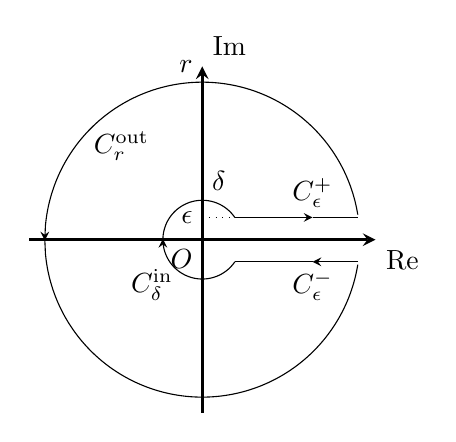
\begin{tikzpicture}[>=stealth]
                \draw[->,line width=1pt] (-2.2,0) -- (2.2,0) node[below right] {Re};
                \draw[->,line width=1pt] (0,-2.2) -- (0,2.2) node[above right] {Im};
                \node[below left] at (0,0) {$O$};
                \draw[domain=-2:1.98, samples=500] plot(\x, {sqrt(4-(\x)^2)});
                \draw[domain=-2:1.98, samples=500] plot(\x, -{sqrt(4-(\x)^2)});
                \draw[domain=-0.5:0.414, samples=500] plot(\x, {sqrt(0.25-(\x)^2)});
                \draw[domain=-0.5:0.414, samples=500] plot(\x, -{sqrt(0.25-(\x)^2)});
                \draw[->] (-0.5,-0.01) -- (-0.5,0.01);
                \draw[->] (-2,0.01) -- (-2,-0.01);
                \draw[->] (0.414,0.282) -- (1.4,0.282);
                \draw (1.4,0.282) -- (1.98,0.282);
                \draw[->] (1.98,-0.282) -- (1.4,-0.282);
                \draw (1.4,-0.282) -- (0.414,-0.282);
                \node[above right] at (0,0.5) {$\delta$};
                \node[above left] at (0,2) {$r$};
                \node[left] at (0,0.282) {$\epsilon$};
                \draw[dotted] (0,0.282) -- (0.414,0.282);
                \node[above] at (1.4,0.282) {$C^+_\epsilon$};
                \node[below] at (1.4,0-.282) {$C^-_\epsilon$};
                \node[below left] at (-0.25,-0.25) {$C_\delta^{\mathrm{in}}$};
                \node[below right] at (-1.5,1.5) {$C_r^{\mathrm{out}}$};
            \end{tikzpicture}
        \end{center}
        これについて,
        \[\int_\gamma e^{\al g(z)}R(z)dz=2\pi i\sum_{a\in\C\setminus\R_+}\Res_a\paren{e^{\al g(z)}R(z)}.\]
        \item[$C_\delta^{\mathrm{in}},C_r^{\mathrm{out}}$上の積分は消える]
        いま,$\abs{e^{\al g(z)}}=e^{\al\Re(z)}=e^{\al\log\abs{z}}=\abs{z}^\al$と,$R$は$z=0$で高々1位の極を持つことと,$\deg Q-\deg P\ge2$とより,
        \[\exists_{M_1\in\R}\exists_{r_1>0}\;\abs{R(z)}\le\frac{M_1}{\abs{z}}\;\on\Delta(0,r_1),\quad\exists_{M_2\in\R}\;\exists_{r_2>0}\;\abs{R(z)}\le\frac{M_2}{\abs{z}^2}\;\on\abs{z}>r_2\]
        であるから,それぞれ
        \begin{align*}
            \Abs{\int_{C_\delta^\mathrm{in}}e^{\al g(z)}R(z)dz}&\le 2\pi\delta\cdot\delta^\al\frac{M_1}{\delta}\xrightarrow{\delta\to0}0.\\
            \Abs{\int_{C_r^\mathrm{out}}e^{\al g(z)}R(z)dz}&\le2\pi\rho\cdot\rho^\al\frac{M_2}{\rho}\xrightarrow{\rho\to\infty}0.
        \end{align*}
        よって,積分路の$r,\delta$の変化に関する連続性により,それぞれの積分は$0$である.
        \item[$C_\ep^+,C_\ep^-$上の積分の値] 
        \[\int_{C^+_\ep+C^-_\ep}e^{\al g(z)}R(z)dz=\int^\rho_\delta e^{\al\log(x+\ep i)}R(x)dx-\int^\rho_\delta e^{\al\log(x-i\ep)}R(x)dx\xrightarrow{\ep\to+0}(1-e^{2\pi i\al})\int^\rho_\delta e^{\al\log x}R(x)dx.\]
    \end{description}
    以上より,$\delta,\rho$についての連続性から,$\to\infty$の場合との整合性を考えると,
    \[\int^\infty_0x^\al R(x)dx=\int^\rho_\delta e^{\al\log x}R(x)dx=\frac{1}{1-e^{2\pi i\al}}\int_\gamma e^{\al g(z)}R(z)dz=\frac{2\pi i}{1-e^{2\pi i\al}}\sum_{a\in\C\setminus\R_+}\Res_a\paren{e^{\al g(z)}R(z)}.\]
\end{Proof}

\begin{example}[対数を使うか,指数関数に変数変換をするか.]
    \[\tcboxmath{I:=\int^\infty_0\frac{dx}{(1+x)x^\alpha}=\frac{\pi}{\sin\al\pi}\qquad(\alpha>0)}\]
    非積分関数$f(z)=(1+z)^{-1}e^{-\alpha\log z}$の極は$z=-1$のみ.その留数は
    \[\Res_{-1}f(z)=\left.e^{-\alpha\log z}\right|_{z=-1}=e^{-\alpha\pi i}\]
    より,
    \[I=\frac{2\pi i}{1-e^{-2\pi i\alpha}}e^{-\alpha\pi i}=\frac{2\pi i}{e^{\pi i\alpha}-e^{-\pi i\alpha}}=\frac{\pi}{\sin\alpha\pi}.\]
\end{example}

\subsection{有理式と対数の積の正軸上の積分}

\begin{tcolorbox}[colframe=ForestGreen, colback=ForestGreen!10!white,breakable,colbacktitle=ForestGreen!40!white,coltitle=black,fonttitle=\bfseries\sffamily,
title=]
    長方形領域の高さを$2\pi$に取ると,$e$の周期性により,$I$とその$-e^{2\pi i\alpha}$倍しか出てこないというテクニックがある.
\end{tcolorbox}

\begin{example}
    \[\tcboxmath{I:=\int^\infty_0\frac{\log x}{x^2+a^2}dx=\frac{\pi^2}{2a}\log a\quad(a>0)}\]
    $\Im\log z\in[0,2\pi)$を満たす$\C\setminus[0,\infty)$上の対数関数を用いて,
    $f(z):=\frac{(\log z)^2}{z^2+a^2}=\frac{(\log z)^2}{(z+ia)(z-ia)}$とおき,
    \[D_{\epsilon}:=\left\{z\in\C\;\middle|\;\epsilon<\abs{z}<\frac{1}{\epsilon},\dist(z,[0,\infty))>\epsilon\right\}\quad(\epsilon>0)\]
    の境界$C$上での積分を考えると,
    \begin{align*}
        \int_Cf(z)dz&=2\pi i\paren{\frac{(\log(ia))^2}{2ai}+\frac{(\log(-ia))^2}{-2ai}}\\
        &=\frac{\pi}{a}\paren{\paren{\log a+\frac{\pi i}{2}}^2-\paren{\log a+\frac{3\pi i}{2}}^2}&\because e^{\log a+\pi i/2}=ai \footnote{計算規則としてはそうであるが,$ai$とは$a$を90度回転したものであるから,成り立つという意味論を考えると良い.}\\
        &=\frac{\pi}{a}(-2\pi i\log a+2\pi^2)
    \end{align*}
    となる.さて,$\epsilon\to 0$の極限を考えると,左辺の積分の,2つの円弧状の積分路上
    での積分は$0$に収束し,実軸上での積分が2つ残る.$\Im z>0$の方は$I$ではなく$\int^\infty_0\frac{(\log x)^2}{x^2+a^2}dx$に収束し,
    $\Im z<0$の場合は
    \[-\int^\infty_0\frac{(\log x+2\pi i)^2}{x^2+a^2}dx=-\int^\infty_0\frac{(\log x)^2}{x^2+a^2}-4\pi iI+4\pi^2\int^\infty_0\frac{dx}{x^2+a^2}\]
    となるから,左辺は総じて$-4\pi iI+4\pi^2\int^\infty_0\frac{dx}{x^2+a^2}$に収束する.
    両辺の虚部を比較すると,
    \begin{align*}
        \frac{-2\pi^2\log a}{a}&=-4\pi I\\
        I&=\frac{\pi^2}{2a}\log a.
    \end{align*}
\end{example}

\subsection{確率論における留数定理}

\begin{proposition}[Gaussian integarl]
    \[\int^\infty_{-\infty}e^{-x^2}dx=\sqrt{\pi}\paren{=\Gamma\paren{\frac{1}{2}}}.\]
\end{proposition}
\begin{Proof}\mbox{}
    \begin{description}
        \item[Fubiniの定理によるトリック] $e^{-x^2}$の可積分性$\int^\infty_{-\infty}e^{-x^2}dx=:I\in\R_{>0}$を仮定する.
        すると,
        \begin{align*}
            I^2&=\paren{\int^\infty_{-\infty}e^{-x^2}dx}\\
            &=\int_{\R^2}e^{-(x+y)^2}dxdy\\
            &=\int^\pi_{-\pi}\int^\infty_{0}e^{-r^2}rdrd\theta\\
            &=\int^\pi_{-\pi}\frac{1}{2}\Square{e^{-r^2}}^\infty_0d\theta=\pi.
        \end{align*}
        \item[Gamma関数への帰着] $u=x^2$と変数変換すると,
        \[\int^\infty_{-\infty}e^{-x^2}dx=\int^\infty_0u^{-1/2}e^{-u}du=\Gamma\paren{\frac{1}{2}}.\]
    \end{description}
\end{Proof}

\chapter{正則関数の表示}

\begin{quotation}
    正則関数の具体的な表示を得たい(と言っても極限の形になるが)という実用的要請に答える.

    例えば有理関数は,部分分数分解と,分母分子の因数分解という2つの分類法があった.
    これは有理型関数の見地から見ると明瞭になる.
    \begin{enumerate}
        \item 部分分数分解とは,有理型関数を,それぞれの極についての主要部の和の形への分解に他ならない.
        \item 因数分解とは,正則関数の,零点$a_n$に関する因子$(1-z/a_n)$の無限積としての表示に他ならない.
    \end{enumerate}
\end{quotation}

\section{部分分数展開}

\begin{tcolorbox}[colframe=ForestGreen, colback=ForestGreen!10!white,breakable,colbacktitle=ForestGreen!40!white,coltitle=black,fonttitle=\bfseries\sffamily,
title=]
    部分分数展開とは,
    $\C$上の有理型関数を,極の主要部を指定することで構成する場合はTaylorの定理から示せるが,
    一般にどのような領域上で似たような構成が可能かの問題は,
    Rungeの定理による正則凸コンパクト集合$K$の特徴付けなどの準備を必要とする.
\end{tcolorbox}

\subsection{$\C$上の有理型関数に関するMittag-Lefflerの定理}

\begin{theorem}
    $\{b_n\}\subset\hatC$を$\infty$に収束する列とし,$P_n\in\C[z]$を定数項のない多項式とする.
    このとき,$b_n$に特異部を$P_n\paren{\frac{1}{z-b_n}}$とする極を持つような有理型関数$f:\C\to\hatC$が存在し,
    ある多項式列$\{p_n\}\subset\C[z]$と整関数$g\in\O(\C)$が存在して
    次の表示を持つ:
    \[f(z)=\sum_{n\in\N}\paren{P_n\paren{\frac{1}{z-b_n}}-p_n(z)}+g(z).\]
\end{theorem}

\subsection{有理型関数の部分分数展開の例}

\begin{tcolorbox}[colframe=ForestGreen, colback=ForestGreen!10!white, breakable ,colbacktitle=ForestGreen!40!white, coltitle=black,fonttitle=\bfseries\sffamily,
    title=有理型関数の部分分数展開]
    整関数$g$が恒等的に$0$である時には,有理型関数の無限和への表示式を得る.
    \begin{enumerate}
        \item 展開したい有理型関数が1位の極を持つ場合は,Gamma関数の収束性の問題に直面するので,
        2位の場合より議論が一筋縄では行かなくなる.
        そこで,微分が$0$になることを示し,元の等式の成立をLiouvilleの定理を通じて示す技法がある.
    \end{enumerate}
    
    それぞれを,有理式でない場合の有理型関数のうち一番簡単なものを例にとって考える.
    いずれも整関数が$0$になる例.
    しかし$\frac{\pi^2}{\sin^2\pi z}$と$\pi\cot\pi z=\pi\frac{1}{\tan\pi z}$とが有理型関数であるとは,随分射程の広い理論を得たものだ.
\end{tcolorbox}

\begin{proposition}[自乗のものは解きやすい]\label{prop-partial-fractional-decomposition}
    \[\tcboxmath{\frac{\pi^2}{\sin^2\pi z}=\sum_{n\in\Z}\frac{1}{(z-n)^2}}\]
\end{proposition}
\begin{Proof}
    $f(z):=\frac{\pi^2}{\sin^2\pi z}$と置く.極は$f^{-1}(\infty)=\Z$である.
    \begin{description}
        \item[特異部の計算] \mbox{}
            \begin{enumerate}
                \item $z=0$では,$z=0$の近傍で消えない正則関数$\varphi,\psi$を用いて,
                \begin{align*}
                    f(z)&=\frac{\pi^2}{\sin^2\pi z}=\frac{\pi^2}{(\pi z)^2\paren{1+z^2\varphi(z)}^2}\\
                    &=\frac{1}{z^2}(1-z^2\psi(z))=\frac{1}{z^2}-\psi(z)
                \end{align*}
                と表せるから,2位の極で主要部$1/z^2$を持つ.
                \item $f(z)$は周期1を持つから,一般の$z=n\in\Z$における主要部は$1/(z-n)^2$となる.\footnote{$z=n$とは$z-n=0$である.従って,周期性(基本周期$1$)とは,変数を$z\mapsto z-n$に変換した場合に同じ値になることをいう.}
            \end{enumerate}
        \item[無限和の一様収束] \mbox{}
            $\sum_{n\in\Z}\frac{1}{(z-n)^2}$が$\C$上で$\hatC$-正則関数に広義一様収束することを示す.
            $\Delta(0,N)$の形をしたコンパクト集合は併呑だから,この上での一様収束を導けば良い.
            級数の有限項を除いた部分が
            \[\sum^\infty_{n=N+1}\frac{1}{\abs{z\pm n}^2}\le\sum^\infty_{n=N+1}\frac{1}{\abs{N-n}^2}\le\sum^\infty_{m=1}\frac{1}{m^2}<\infty\]
            であることから,Weierstrassの$M$-判定法よりわかる.
        \item[整関数分の差は消える]
            こうして,$g(z):=f(z)-\sum_{n\in\Z}\frac{1}{(z-n)^2}$と定めると,これは極の主要部が取り去られており,任意の点で冪級数展開を許すために整関数である.
            これが$g=0$であることを示せば,定理\ref{thm-partial-fraction-decomposition}より結論を得る.
            これは次のように行う.$g$が$[0,1]\times(-\infty,\infty)$で有界であることを示せば周期性より$\C$上で有界で,Liouvilleの定理から定数関数であることがわかり,$\infty$での値から$g=0$であることを結論づけられる.
            \begin{enumerate}
                \item $x\in\R$に依らず,$f$が$\abs{\Im z}\to\infty$について$0$に一様収束$\lim_{\abs{y}\to\infty}\sup_{x\in\R}f(x+iy)=0$することを示す.
                $\sin \pi(x+iy)=\frac{e^{\pi i(x+iy)}-e^{-\pi i(x+iy)}}{2i}$であるから,
                \begin{align*}
                    \abs{2\sin\pi(x+iy)}&=\Abs{e^{\pi i(x+iy)}-e^{-\pi i(x+iy)}}\\
                    &=\Abs{e^{-\pi y}e^{\pi ix}-e^{\pi y}e^{-x\pi i}}\\
                    &=\Abs{e^{2\pi ix}e^{-\pi y}-e^{\pi y}}&\because 両辺に\times\Abs{e^{\pi is}}\\
                    &\ge\Abs{e^{-\pi y}-e^{\pi y}}&等号成立はx\in\Z のとき\\
                    \therefore\quad 0<\frac{1}{\abs{\sin\pi(x+iy)}}&\le\frac{2}{\Abs{e^{-\pi y}-e^{\pi y}}}
                \end{align*}
                より,
                \begin{align*}
                    \abs{f(x+iy)}&=\Abs{\frac{\pi^2}{\sin^2\pi(x+iy)}}\le(2\pi^2)\Abs{e^{-\pi y}-e^{\pi y}}\xrightarrow{\abs{y}\to\infty}0.
                \end{align*}
                \item $x\in[0,1]$に依らず,命題の式の右辺が$\abs{\Im z}\to\infty$について$0$に一様収束$\lim_{\abs{y}\to\infty}\sup_{x\in[0,1]}\sum_{n\in\Z}\abs{x+yi-n}^{-2}=0$することを示す.
                いま,任意の$\epsilon>0$に対して,
                \[\sum_{\abs{n}>N}\abs{x+iy-n}^{-2}\le\sum_{\abs{n}>N}\abs{x-n}^{-2}<\epsilon\]
                である.残りは$\abs{y}>\delta$を満たす$\delta$について
                \[\sum_{\abs{n}\le N}\abs{x+iy-n}^{-2}<(2N+1)\delta^{-2}\]
                が成り立つことより,$\delta$を十分大きくとれば$\abs{n}\le N$の和も$\epsilon$以下に出来る.総じて,
                \[\abs{y}>\delta\Rightarrow\sum_{n\in\Z}\frac{1}{(z-n)^2}\le 2\epsilon\]
                を得た.
                \item 以上より,$\lim_{\abs{y}\to\infty}\sup_{x\in[0,1]}g(x+iy)=0-0=0$.よって,$g$は帯状集合$[0,1]\times(-\infty,\infty)$上で有界で,$g$の周期$1$より,結局$\C$上で有界である.よって,Liouvilleの定理\ref{thm-Liouville}より,$g$は定数関数であるが,$\abs{y}\to\infty$の時の値より,$g=0$.
            \end{enumerate}
    \end{description}
\end{Proof}

\begin{proposition}[1位の極を持つもの]
    \[\tcboxmath{\pi\cot\pi z=\frac{1}{z}+\sum_{n\in\Z\setminus\{0\}}\paren{\frac{1}{z-n}+\frac{1}{n}}.}\]
\end{proposition}
\begin{Proof}
    $\pi\cot\pi z$の$n\in\Z$での極の主要部は$\frac{1}{z-n}$であるが,
    級数$\sum_{n\in\Z\setminus\{0\}}\frac{1}{z-n}$は収束しない.
    \begin{description}
        \item[無限和のデザイン] 同じ無限和を,
        \[\frac{1}{z}+\sum_{n\in\Z\setminus\{0\}}\paren{\frac{1}{z-n}+\frac{1}{n}}=\frac{1}{z}+\sum_{n\in\Z\setminus\{0\}}\frac{z}{n(z-n)}<\frac{1}{z}+\sum_{n\in\Z\setminus\{0\}}\frac{z}{n^2}.\]
        と考えると,優級数が見つかるために,収束を示せる.これは有理型関数に広義一様収束する.
        従って,整関数$g$が存在して,
        \[\pi\cot\pi z=\frac{1}{z}+\sum_{n\in\Z\setminus\{0\}}\paren{\frac{1}{z-n}+\frac{1}{n}}+g(z).\]
        \item[$g=0$:今回は微分で解決する]
        両辺を微分すると,
        \[-\frac{\pi^2}{\sin^2\pi z}=-z^2-\sum_{n\in\Z\setminus\{0\}}\frac{1}{(z-n)^2}+g'(z)\]
        より,命題\ref{prop-partial-fractional-decomposition}より,$g'(z)=0$だから,$g$は定数関数である.
        ここで,
        \begin{align*}
            \sum_{n\in\Z\{0\}}\paren{\frac{1}{z-n}-\frac{1}{n}}&=\sum^\infty_{n=1}\paren{\paren{\frac{1}{z-n}-\frac{1}{n}}+\paren{\frac{1}{z+n}+\frac{1}{n}}}\\
            &=\sum^\infty_{n=1}\frac{2z}{z^2-n^2}
        \end{align*}
        より,
        \[\pi\cot\pi z=\frac{1}{z}+\sum^\infty_{n=1}\frac{2z}{z^2-n^2}+g\]
        であるが,左辺は奇関数,$\frac{1}{z}+\sum^\infty_{n=1}\frac{2z}{z^2-n^2}$も奇関数なので,$g=0$.
    \end{description}
\end{Proof}
\begin{remarks}
    $\cot$というのは,$\frac{1}{\sin\pi z}$だと周期が$2$になり,$1$だと$(-1)^n$が付くのがわずわらしい.これを消すためのデザインである.
\end{remarks}

\begin{example}\mbox{}
        \[\tcboxmath{\frac{\pi}{\sin\pi z}=\lim_{m\to\infty}\sum_{\abs{n}\le m}\frac{(-1)^n}{z-n}.}\]
        これは有理型関数$\frac{\pi}{\sin\pi z}$の$n\in\Z$での主要部が$\frac{(-1)^n}{z-n}$であることから予想がつく.
    右辺が一様収束することは,$\pm$の対をセットで考えると
    \[\lim_{m\to\infty}\sum_{\abs{n}\le m}\frac{(-1)^n}{z-n}=\frac{1}{z}+\sum^\infty_{n=1}(-1)^n\frac{2z}{z^2-n^2}\]
    であることからわかる.さて,等式は,\textbf{偶数と奇数で分ける}と見えてくる:
    \begin{align*}
        \sum_{\abs{n}\le m}\frac{(-1)^n}{z-n}&=\sum_{\abs{2n}\le m}\frac{1}{z-2n}-\sum_{\abs{2n+1}\le m}\frac{1}{z-2n-1}\\
        &=\frac{1}{2}\sum_{\abs{2n}\le m}\frac{1}{z/2-n}-\frac{1}{2}\sum_{\abs{2n+1}\le m}\frac{1}{(z-1)/2-n}\\
        \xrightarrow{m\to\infty}&\frac{1}{2}\pi\cot\pi\frac{z}{2}-\frac{1}{2}\pi\cot\pi\frac{z-1}{2}\\
        &=\frac{\pi}{2}\paren{\frac{\cos\frac{\pi}{2}z}{\sin\frac{\pi}{2}z}-\frac{\cos\paren{\frac{\pi}{2}z-\frac{\pi}{2}}}{\sin\paren{\frac{\pi}{2}z-\frac{\pi}{2}}}}\\
        &=\frac{\pi}{2}\paren{\frac{\cos\frac{\pi}{2}z}{\sin\frac{\pi}{2}z}+\frac{\sin\frac{\pi}{2}z}{\cos\frac{\pi}{2}z}}\\
        &=\frac{\pi}{2}\frac{1}{\sin\frac{\pi}{2}\cos\frac{\pi}{2}}=\frac{\pi}{2}\frac{2}{\sin\pi z}=\frac{\pi}{\sin\pi z}.
    \end{align*}
\end{example}

\begin{example}[極を二次元的に持つ有理型関数は楕円函数]
    $\Z+i\Z$に極を持つ有理型関数
    \begin{align*}
        f(z)&=\sum_{n,m\in\Z}\frac{1}{(z-n-im)^k}\quad(k\ge 3)
    \end{align*}
    は,$f(z+1)=f(z+i)=f(z)$をみたし,$1,i$を周期とする.
    このような有理型関数を楕円関数という.
    これはRiemann球面ではなく,Torus上の有理型関数とみなせばよく,
    この大地の上の関数の研究を楕円関数論という.
    三角関数は楕円関数の退化と考えられる.
\end{example}

\section{一般のMittag-Lefflerの定理}

\subsection{Rungeの近似定理}

\begin{theorem}[Runge]
    $K\compsub \Om\osub\C$とする.次の3条件は同値.
    \begin{enumerate}
        \item $K$の近傍で正則な関数は,$\O(\Om)$で$K$上一様に近似可能である.
        \item $\Om\setminus K$は$\Om$上相対コンパクトな連結成分を持たない.
        \item $K$は正則凸である:$\forall_{z\in\Om\setminus K}\;\exists_{f\in\O(\Om)}\;\abs{f(z)}>\sup_{K}\abs{f}$.
    \end{enumerate}
\end{theorem}

\begin{corollary}[正則関数の一様近似]
    任意のコンパクト集合$K\subset\C$が連結ならば,この近傍で定義された正則関数は多項式によって一様近似可能である.
\end{corollary}
\begin{Proof}
    $\Om=\C$と取ると,$\O(\C)$は多項式で一様近似可能である.
\end{Proof}

\subsection{正則凸性}

\begin{definition}
    コンパクト集合$\wh{K}\subset D$に対して,$\wh{K}_D:=\Brace{z\in D\mid\forall_{f\in\O(D)}\;\abs{f(z)}\le\norm{f}_K}$を\textbf{正則凸包}という.
\end{definition}

\begin{theorem}
    $\wh{K}_D$は,$K$と,$D\setminus K$の$D$上相対コンパクトな連結成分との合併である.
\end{theorem}

\subsection{有理型関数}

\begin{notation}
    $\O_z$を正則関数の芽のなす複素線型位相空間とし,その元を$f_z\in\O_z$と表す.$f_z=g_z$とは,$f,g$が$z$の近傍で局所的に等しいことをいう.
    $\O_z$は環の構造も持ち,非自明な零因子がない(整域)から,商体$M_z:=\Frac(\O_z)$を得る.
    商体の普遍性は,任意の体$F$への単射準同型$f:\O_z\to F$は,一意な$M_z$上への延長を持つことである.
\end{notation}

\begin{definition}[meromorphic function]
    $\Om\osub\C$上の有理型関数とは,ファイバー$\sqcup_{z\in\Om}M_z\to\Om$の切断$\varphi:\Om\to\cup_{z\in\Om}M_z$であって,任意の$z\in\Om$に対して,その近傍上の正則関数$f,g$が存在して$\varphi=f_z/g_z$と局所的に表せるものをいう.
    有理型関数の全体を$M(\Om)$であらわすと,標準的な単射$\O(\Om)\mono M(\Om)$が存在する.$M(\Om)$は環をなす.$\Om$の任意の成分上で恒等的に零とはならないならば,$M(\Om)$内で可逆である.
\end{definition}

\begin{theorem}
    $F$を$\zeta$の近傍上の有理型関数とする.このとき,ある正則関数$G\in\O$と定数$\{A_k\}\subset\C$が一意的に存在して,ある$\zeta$の近傍上で
    \[F(z)=\sum^n_{k=1}\frac{A_k}{(z-\zeta)^k}+G(z).\]
\end{theorem}

\subsection{Mittag-Lefflerの定理}

\begin{theorem}[Mittag-Leffler]
    次の同値な2条件が成り立つ:
    \begin{enumerate}
        \item 離散集合$\{z_j\}\subset\Om$と,それぞれの近傍での有理型関数$f_j\in\wt{M}_{z_j}$について,ある有理型関数$f\in M(\Om)$が存在して,$\Om\setminus\{z_j\}$上正則で,$f-f_j$が各$z_j$の近傍で正則な($f_j$を主要部とする)ものが存在する.
        \item 可算な開被覆$\Om=\cup_{j\in\N}\Om_j$に対して,$f_j\in M(\Om_j)$が与えられていて,条件$f_j-f_k\in\O(\Om_j\cap\Om_k)$を満たすとする.このとき,ある$f\in M(\Om)$が存在して,$\forall_{j\in\N}\;f-f_j\in\O(\Om_j)$.
        \item Cauchy-Riemann作用素$\pp{}{\o{z}}:C^\infty(\Om)\to C^\infty(\Om)$は全射である.
        \item 可算な開被覆$\Om=\cup_{j\in\N}\Om_j$に対して,$g_{jk}\in\O(\Om_j\cap\Om_k)$が与えられていて,
        \[g_{jk}=-g_{kj},\; g_{jk}+g_{kl}+g_{lj}=0\;\on\Om_j\cap\Om_k\cap\Om_l\]
        を満たすならば,ある$g_j\in A(\Om_j)$が存在して,$g_{jk}=g_k-g_j\;\on\Om_j\cap\Om_k$を満たす.
    \end{enumerate}
\end{theorem}
\begin{remarks}
    もちろん,(3)の方法で多変数の場合に拡張することとなる.
\end{remarks}

\subsection{Weierstrassの定理}

\begin{theorem}
    $\{z_j\}\subset\C$を離散集合,$\{n_j\}\subset\Z$を整数列とする.このとき,ある$f\in M(\Om)$が存在して,$f\in\O(\Om\setminus\{z_j\})$は零にならず,任意の$z_j$の近傍で$f(z)(z-z_j)^{-n_j}$が解析的で零を取らないものが存在する.
\end{theorem}

\begin{corollary}
    $\Om\osub\C$上の任意の有理型関数に対して,ある正則関数$f,g$が存在して$f/g$と表せる.
\end{corollary}


\section{無限積展開}

\subsection{定義}

\begin{tcolorbox}[colframe=ForestGreen, colback=ForestGreen!10!white,breakable,colbacktitle=ForestGreen!40!white,coltitle=black,fonttitle=\bfseries\sffamily,
title=]
    無限積$\prod_{n\in\N}z_n$が収束するとは,$z_n\ne0\;\fe$で,これらを除いた部分積の極限が$\R\setminus\{0\}$上収束することをいう.
\end{tcolorbox}

\begin{definition}[複素数の無限積の収束]\mbox{}
    \begin{enumerate}
        \item 
    複素数列$(z_n)_{n\in\N}$に対し,無限積$\prod_{n\in\N}z_n$が収束するとは,
    \[\exists N\in\N,\;\exists \alpha_N\in\C,\;\alpha_N=\lim_{m\to\infty}\prod_{n=N}^mz_n\ne 0\]
    が成り立つことをいう.
        \item この時,無限積の極限値を$\prod_{n\in\N}z_n:=\al_N\prod^{N-1}_{k=1}z_k$とする.
    \end{enumerate}
\end{definition}

\begin{definition}[関数列の無限積の収束]\mbox{}
    \begin{enumerate}
        \item 関数列$(f_n)$の無限積$\prod^\infty_{n=1}f_n$が収束するとは,$\exists_{N\in\N}\;F_N(z):=\lim_{m\to\infty}\prod^m_{n=N}f_n(z)$が収束し,零点を持たない.
        \item 無限積を$\prod^\infty_{n=1}f_n:=F_N\prod^{N-1}_{n=1}f_n$と定め,$F_m$が一様収束するとき,無限積が一様収束するという.
    \end{enumerate}
\end{definition}

\begin{lemma}[対数微分]
    領域$D$上の零でない正則関数の列$(f_n)$に対して,$F_n:=\prod^\infty_{n=1}f_n$は広義一様収束するとする.
    このとき,$F$は正則であり,
    \[\frac{F'}{F}=\prod^\infty_{n=1}\frac{f'_n}{f_n}\]
    が成り立つ.
\end{lemma}

\subsection{収束の特徴付け}

\begin{lemma}[無限積の収束に必要な自明な必要条件]
    無限積$\prod_{n=1}^\infty z_n$が収束するならば,$\lim_{n\to\infty}z_n=1$である.
\end{lemma}
\begin{Proof}
    ある$M\in\N$が存在して,$P_m:=\prod^m_{n=M}z_n$は$\al\ne0$に収束する.このとき,
    \[\lim_{m\to\infty}z_m=\lim_{m\to\infty}\frac{P_m}{P_{m-1}}=\frac{\al}{\al}=1.\]
\end{Proof}

\begin{remark}
    そこで,無限積を$\prod^\infty_{n=1}(1+a_n)$と見ることを考える.これが収束するには,$\lim_{n\to\infty}a_n=0$が必要.
    無限積の収束の判定では最初の有限項は無視して良いから,最初から$\abs{a_n}<1$を仮定しても実用性を失わない.
    すると,列$(1+a_n)$は右半平面上の点列である.
    $z$が負の実軸上にないときは,$\log z$を虚部の値域が
    $(-\pi,\pi)$
    に含まれるように取れる.
    これを対数の主値といい,$\Log:\Logdomain\to\C$で表すのであった\ref{def-principle-value-of-log}.
\end{remark}

\begin{theorem}[無限積が収束することの特徴付け]
    $\Delta$内の点列$(a_n)$について,次の2条件は同値.
    \begin{enumerate}
        \item $\prod^\infty_{n=1}(1+a_n)$は収束する.
        \item $\sum^\infty_{n=1}\Log(1+a_n)$は収束する.
    \end{enumerate}
    ただし,$\Log:\Logdomain\to\C$は主値とした:$\pi<\Im\log(1+a_n)\le\pi$.
\end{theorem}

\begin{proposition}
    $\Delta$内の点列$(a_n)$について,次の3条件は同値.
    \begin{enumerate}
        \item $\sum^\infty_{n=1}\abs{a_n}<\infty$.
        \item $\sum^\infty_{n=1}\abs{\Log(1+a_n)}<\infty$.
        \item $\prod_{n=1}^\infty(1+a_n)$が絶対収束する.
    \end{enumerate}
\end{proposition}

\begin{theorem}
    関数列$(f_n)$について,$\sum_{n\in\N}f_n$が一様収束すれば,$\prod_{n\in\N}(1+f_n)$も一様収束する.
\end{theorem}

\subsection{整関数に関するWeierstrassの定理}

\begin{theorem}[Weierstrass]\mbox{}\label{thm-Weierstrass-pre}
    \begin{enumerate}
        \item $\C$内に集積点を持たない点列$\{a_n\}$に対して,整関数$f:\C\to\C$であって,その零点が重複度もこめて$\{a_n\}$と一致するものが存在する.
        \item さらに$a_1=a_2=\cdots=a_m=0,a_n\ne0(n>m)$とするとき,多項式の列$(P_n)_{n=m+1}^\infty$が存在して,\[f(z)=z^me^{g(z)}\prod_{n=m+1}^\infty\paren{1-\frac{z}{a_n}}e^{P_n(z)}\]
        と表示できる.ここで$g(z)$は零点を持たない整関数で,無限積は
        広義一様収束する
    \end{enumerate}
\end{theorem}
\begin{Proof}
    一般の複素領域における証明は\ref{thm-Weierstrass-zero}.
    ここでは構成的に証明する.
\end{Proof}

\begin{example}[genus]
    $\N$に1位の零点を持つ整関数は,$P_n(z)=z/n$ととれて,次のような積表示を持つ:
    \[\tcboxmath{e^{g(z)}\prod^{\infty}_{n=1}\paren{1-\frac{z}{n}}e^{z/n}}\]
    これは,$(P_n)$を常に1次式として取っている.
    実は,ある自然数$k\in\N$に対して,$0$でない$a_n$に関する和$\sum_{n\in\N,a_n\ne0}\abs{a_n}^{-k-1}$が有限であるとき,$P_n(z)$として$k$次式を取れる.
    このような$k\in\N$の最小値を,列$(a_n)$の\textbf{種数}といい,$a_n=n$の場合,種数は1である.
    種数次の多項式を用いた無限積表示を特に\textbf{基本乗積}という.
\end{example}

\begin{corollary}[$\C$上の有理型関数とは,2つの整関数の商である]
    $\C$上の有理型関数$F:\C\to\hatC$は,2つの整関数$f,g$の商$f/g$として表せる.
\end{corollary}

\begin{example}
    \[\tcboxmath{\sin\pi z=\pi z\prod_{n\in\Z\setminus\{0\}}\paren{1-\frac{z}{n}}e^{z/n}=\pi z\prod^\infty_{n=1}\paren{1-\frac{z^2}{n^2}}}\]
\end{example}

\subsection{一般のWeierstrassの定理}

\begin{tcolorbox}[colframe=ForestGreen, colback=ForestGreen!10!white,breakable,colbacktitle=ForestGreen!40!white,coltitle=black,fonttitle=\bfseries\sffamily,
title=]
    零点についても,全く同様な構成が可能で,これは零点に限らない(補間定理).
\end{tcolorbox}

\begin{theorem}[Weierstrass]\ref{thm-Weierstrass-zero}
    領域$D\subset\C$内の$D$上に集積点を持たない\footnote{$D$の点であって,全ての開近傍が$Z$に交わってしまうような点がない.任意の$z\in D$が$Z\cup\{z\}$の孤立点であることをいう}離散部分集合$Z\subset D$を考える.写像$m:Z\to\N_+$に対して,$f\in\O(D)$であって,$f$の零点は$Z$のみで,$a\in Z$での零点の位数が$m(a)$であるようなものが存在する.
\end{theorem}

\begin{corollary}[補間定理]\ref{thm-interpolation}
    $D\subset\C$を領域,$Z\subset D$をその離散部分集合とする.
    任意の関数$f:Z\to\C$は正則関数$\o{f}:D\to\C$に延長できる.
\end{corollary}

\section{Gamma関数}

\subsection{定義と基本的性質}

\begin{notation}
    $R:=\Brace{z\in\C\mid\Re z>0}$を右半平面とする.$R+\al=\Brace{z\in\C\mid\Re z>\al}$とする.
\end{notation}

\begin{proposition}
    \[\Gamma(z):=\int^\infty_0e^{-t}t^{z-1}dt\quad(z\in R)\]
    とする.
    \begin{enumerate}
        \item $\Gamma$は右半平面$R$上で広義一様収束し,正則関数を定める.
        \item $\Gamma(z+1)=z\Gamma(z)\;\on R$が成り立つ.特に,$\forall_{n\in\N}\;\Gamma(n)=(n-1)!$.
    \end{enumerate}
\end{proposition}

\subsection{有理型関数としての延長}

\begin{definition}
    任意の$m\in\N$に対して,
    \[\Gamma_{-m}(z):=\frac{\Gamma(z+m)}{z(z+1)(z+2)\cdots(z+m-1)}\;(\on\;R-m)\]
    と定めると,各$\Gamma_{-m}:R-m\to\hatC$は有理型であり,$\forall_{n<m}\;\Gamma_{-n}=\Gamma_{-m}\;\on\;R-n$上で一致し,$\Gamma$と$R$上で一致する.
    これの極限として有理型関数$\Gamma:\C\to\hatC$を得る.
\end{definition}

\begin{proposition}\mbox{}
    \begin{enumerate}
        \item $\Gamma^{-1}(\infty)=\Brace{0,-1,-2,-3,\cdots}$であり,それぞれ1位の極である.
        \item $-n$での留数は
        \[\Res_{-n}\Gamma(z)=\Res_{-n}\frac{\Gamma(z+n+1)}{z(z+1)\cdots(z+n)}=\frac{(-1)^n}{n!}.\]
    \end{enumerate}
\end{proposition}

\begin{theorem}[反転公式]
    有理型関数の空間$M(\C)$上で,次の等式が成り立つ:
    \[\Gamma(z)\Gamma(1-z)=\frac{\pi}{\sin \pi z}\; M(\C).\]
    特に,$\Gamma$は零点を持たない.また,$\Gamma(1/2)=\sqrt{\pi}$.
\end{theorem}

\begin{proposition}\mbox{}
    \begin{enumerate}
        \item $\frac{1}{\Gamma(z)}=\pi\Gamma(1-z)\sin\pi z$は整関数であり,$\{0,-1,-2,\cdots\}$に1位の零点を持つ.
        \item 次の無限積展開を持つ:
        \[\frac{1}{\Gamma(z)}=ze^{g(z)}\prod^\infty_{n=1}\paren{1+\frac{z}{n}}e^{-z/n},\quad g(z)=\gamma z,\;\gamma:=\lim_{m\to\infty}\paren{\sum^m_{n=1}\frac{1}{n}-\log m}\in\R.\]
        \item 次の表示を持つ:
        \[\Gamma(z)=\lim_{n\to\infty}\frac{n^zn!}{z(z+1)\cdots(z+n)}.\]
    \end{enumerate}
\end{proposition}
\begin{Proof}
    (3)を示すことで(2)はすぐに従う.
\end{Proof}

\section{Stirlingの公式}

\section{Zeta関数}

\subsection{定義と積表示}

\begin{proposition}
    \[\zeta(z):=\sum^\infty_{n=1}n^{-z}\quad(z\in R+1)\]
    とする.$R+1=\Brace{\Re z>1}$上で一様収束し,正則関数を定める.
\end{proposition}

\begin{theorem}[Euler積表示]
    素数を$2=p_1<p_2<\cdots$とする.このとき,
    \[\zeta(z)\prod^\infty_{n=1}\paren{1-\frac{1}{p_n^z}}=1\;\on\;R+1.\]
    特に,$\zeta$は$R+1$上に零点を持たない.また,$\sum_{n\in\N}p^{-1}_n=\infty$で,素数は無限個ある.
\end{theorem}
\begin{remarks}
    このことは,$p_n\sim n^a\;(a>1)$の分布に従わないことを示唆する(さもなくば収束する).
    実際には,$p_n\sim n\log n$であることが,$\zeta$の$\partial(R+1)$での挙動から知られている.
\end{remarks}

\subsection{解析接続による有理型関数への延長}

\begin{lemma}
    命題(1)の
    右辺の積分に関連して,次の等式が成り立つ:
    \[\frac{\zeta(z)}{\Gamma(1-z)}=\frac{1}{2\pi i}\int_C\frac{w^{-z-1}}{e^{w}-1}dw=2(2\pi)^{z-1}\sin(z\pi/2)\sum_{m=1}^\infty m^{z-1}=2(2\pi)^{z-1}\sin(z\pi/2)\zeta(1-z)\;\on\; z\in\C\]
    ただし,$C:=\partial\Brace{w\in\C\mid\dist(w,\R_+)<\ep}$とした.
    特に,左半平面$-R$には,$\zeta(0)=1/2,\zeta(-2m)=0$以外の零点はない.
\end{lemma}

\begin{proposition}[関数等式]\mbox{}
    \begin{enumerate}
        \item Gamma関数とZeta関数について,次の等式が成り立つ:
        \[\zeta(z)\Gamma(z)=\int^\infty_0\sum^\infty_{n=1}e^{-ny}y^{z-1}dy=\int^\infty_0\frac{y^{z-1}}{e^y-1}dy=:I(z)\;\on\;R+1.\]
        \item 
        命題(1)の
        右辺の積分に関連して,次の等式が成り立つ:
        \[\frac{\zeta(z)}{\Gamma(1-z)}=\frac{1}{2\pi i}\int_C\frac{w^{-z-1}}{e^{w}-1}dw=2(2\pi)^{z-1}\sin(z\pi/2)\sum_{m=1}^\infty m^{z-1}=2(2\pi)^{z-1}\sin(z\pi/2)\zeta(1-z)\;\on\; z\in\C\]
        ただし,$C:=\partial\Brace{w\in\C\mid\dist(w,\R_+)<\ep}$とした.
        \item 特に,$\C$の全域で有理型,$\C\setminus\{1\}$上で正則な関数
        \[\zeta(z)=2(2\pi)^{z-1}\sin(\pi z/2)\Gamma(1-z)\zeta(1-z)\]
        に延長され,また
        左半平面$-R$には,$\zeta(0)=1/2,\zeta(-2m)=0$以外の零点はない.
    \end{enumerate}
\end{proposition}
\begin{remarks}
    こうして,$-R$と$R+1$における零点には協力な研究道具がある.
    しかし,帯領域$0\le \Re z\le 1$における零点の研究は困難を極める.
    WienerによるTauber型の定理と$\Re s=1$上で零点が存在しないことは同値である.
\end{remarks}

\begin{corollary}
    $n$以下の素数の個数を$\pi(n)$とすると,
    \[\lim_{n\to\infty}\frac{\pi(n)}{n/\log n}=\lim_{n\to\infty}\frac{p_n}{n\log n}=1.\]
\end{corollary}

\subsection{普遍性}

\begin{tcolorbox}[colframe=ForestGreen, colback=ForestGreen!10!white,breakable,colbacktitle=ForestGreen!40!white,coltitle=black,fonttitle=\bfseries\sffamily,
title=]
    任意の正則関数は,$\zeta$の平行移動によって一様近似出来る.
    これはWeierstrassの多項式という関数代数のクラスで近似する結果に対して,単一の関数で正則関数のクラスを近似している.\footnote{中村耕二『ゼータ関数の普遍性について』}
\end{tcolorbox}

\begin{proposition}[Bohr-Courant (1914)]
    任意の$\sigma\in(1/2,1]$に対して,
    \begin{enumerate}
        \item 集合$\Brace{\zeta(\sigma+it)\in\C\mid t\in\R}$は$\C$上稠密である.
        \item 集合$\Brace{\log\zeta(\sigma+it)\in\C\mid t\in\R}$は$\C$上稠密である.
    \end{enumerate}
\end{proposition}

\begin{proposition}[Voronin]
    任意の$\sigma\in(1/2,1],m\in\N$に対して,
    \[\Brace{(\zeta(\sigma+it),\zeta'(\sigma+it),\cdots,\zeta^{(m-1)}(\sigma+it))\in\C^m\mid t\in\R}\]
    は$\C^m$上稠密である.
\end{proposition}

\begin{theorem}[Voronin (1975)]
    $K\compsub\Brace{z\in\C\mid1/2<\Re z<1}$を単連結コンパクト集合,$f:K\to\C$を零点をもたない正則関数とする.
    このとき,$A(T;f,\ep):=\Brace{\tau\in[0,T]\mid\sup_{z\in K}\abs{\zeta(z+i\tau)-f(z)}<\ep}$について,
    \[\forall_{\ep>0}\;\liminf_{T\to\infty}\frac{1}{T}m(A(T;f,\ep))>0.\]
\end{theorem}
\begin{remarks}
    Riemannの条件収束定理は,条件収束級数は$\R$の任意の値を表現する普遍性を主張していると見れる.
    この方向の拡張と思える結果が
    \begin{proposition}[Fekete (1915)]
        ある実無限級数$\sum_{n\in\N}a_nx^n$が存在して,任意の$f(0)=0$を満たす連続関数$f\in C([-1,1])$について,自然数列$\{m_k\}\subset\N$が存在して,一様に$\sum_{n=1}^{m_k}a_nx^n\to f(x)$が成り立つ.
    \end{proposition}
    \begin{proposition}[Brikhoff]
        整関数$\psi:\C\to\C$が存在して,任意の整関数$f:\C\to\C$に対して,複素数列$\{a_k\}\subset\C$が存在して,コンパクト一様に$\psi(z+a_k)\to f(z)$が成り立つ.
    \end{proposition}
    この種の現象を,Marcinkiewiczは解析学における普遍性と呼んだ.
    しかしVoronin (75)の出現以前の普遍的関数は,命題の主張では隠されているように,極めて人工的なものであった.
\end{remarks}

\subsection{Bohr-Jessenの極限定理}

\begin{tcolorbox}[colframe=ForestGreen, colback=ForestGreen!10!white,breakable,colbacktitle=ForestGreen!40!white,coltitle=black,fonttitle=\bfseries\sffamily,
title=]
    確率測度の言葉で再定式することが出来,現在ではBagchiによる確率論的な証明が主流となっている.
    そもそも,普遍性定理は$\zeta(s+it)\;(t\in\R)$の軌道が$H(D)$上稠密であることを主張するので,大変エルゴード的な香りのする消息である.
\end{tcolorbox}

\begin{notation}
    $A\subset\C$をJordan可測とする.
    \[V(T,A):=m(\Brace{\tau\in[0,T]\mid\log\zeta(\sigma+i\tau)\in A})\]
\end{notation}

\begin{theorem}[Bohr-Jessen]
    \[\forall_{\sigma>1/2}\;W(A)=\lim_{T\to\infty}\frac{V(T,A)}{T}\in\R_+\]
    は絶対連続な測度を定める.
\end{theorem}

\begin{notation}
    $A\subset\C$をBorel集合,
    \[P_{T,\sigma}(A)=\frac{1}{T}m(\Brace{\tau\in[0,T]\mid\zeta(\sigma+i\tau)\in A})\]
    で$\C$上の確率測度を定める.
    これは$T\to\infty$の極限である確率測度$P_\sigma$に弱収束する.
    これを関数空間に持ち上げることを考える.
    $D:=\Brace{z\in\C\mid1/2<\Re z<1}$上の正則関数の全体にコンパクト一様収束の位相を入れたものを$H(D)$とする.
    $\Om:=\prod_{p\in\P}\partial\Delta$とするとコンパクトAbel群となり,全測度が1のHaar測度$m_H$が存在し,$(\Om,\B(\Om),m_H)$は確率空間になる.
    ただし,$\P$は素数全体の集合,$\om(p):=\pr_p:\Om\to\partial\Delta$を射影とする.
    \[\zeta(s,\om):=\prod_{p\in\P}(1-\om(p)p^{-s})^{-1}\]
    は$D$上概収束し,$H(D)$-値確率変数となる.
    その押し出す分布を$P_\zeta(A):=m_H(\zeta^{-1}(A))$とし,
    \[P_T(A):=\frac{1}{T}m(\Brace{\tau\in[0,T]\mid\zeta(s+i\tau)\in A})\]
    も確率測度となる.
\end{notation}

\begin{theorem}[Bagchi]
    $P_T\Rightarrow P_\zeta$.
\end{theorem}
\begin{Proof}
    特性関数のexplicitな計算による弱収束測度の存在証明と,Prokhorovの定理,エルゴード理論のBrikhoff-Khinchinの定理など.
\end{Proof}

\begin{lemma}
    $\sum_{p\in\P}f_p(s)$の形の$H(D)$上で収束する無限級数全体のなす集合は,$H(D)$上稠密である.
\end{lemma}

\chapter{Cauchy-Riemann方程式}

\begin{quotation}
    Cauchy-Riemann方程式を偏微分方程式として考察する理論を,歴史的に自然な出発点として
    Mittag-Lefflerの定理から始める.極という特異点の言葉を避けるため,貼り合わせの言葉で同値換言する.
    さらに有理型関数への言及を避けるため,Cousinの第一問題という純粋に正則関数についての問題に還元する(同値ではない,Mittag-Lefflerの定理の拡張になっている).
    Cousinの第一問題は開被覆を任意に取る問題設定の局所性が煩雑なので,$\Cinf$-関数の世界を借りることによって偏微分方程式の解の存在問題に帰着する.
    Cousinの問題が,一変数と多変数の世界を繋ぐ軸となる.
\end{quotation}

\section{偏微分方程式論}

\begin{history}[岡潔]
    「Stein多様体上の解析的な問題には位相的な障害しかない」ことを岡の原理という(第三論文でのテーマ).
    \begin{quote}
        Cousinの第二問題だけは未知の位相的条件を明らかにすることが残されているが,多分本質的困難はないであろうと予想していたのである.

        結果はその通りであった.しかも,今第三者として見直してみると実に見事な出来栄えである.主定理はこう云っているのである.

        二複素変数の空間に於て,単葉,連結,有限な正則領域内に零点(複数)が与えられたとき,若し非解析解があるならば解析解もある.
        
        『春雨の曲』第七稿
    \end{quote}
    岡潔はLeviの問題に取り組んで世界で初めて解決したが,後年にLars Valter Hörmander 31-12が関数解析と偏微分方程式の手法によって$\o{\partial}$-問題を解決することの帰結として解き直した.
    Hörmanderの教科書に記述がある内容である.
    $\partial_z$が全射を定める空間を単連結というのであった.
    $\o{\partial}$が全射を定める空間を考えることで解決する.
    関数解析の勝利であるか?
    領域化された議論と「その上の関数」という空間に対する位相解析への導入.
    作用素$\partial_z$を全射にする領域$D$を単連結といい,作用素$\partial_{\o{z}}$を全射にする領域$D$を
\end{history}

\begin{history}[Hormander]
    偏微分方程式論の新たな2つの進展が,複素解析学に寄与した.
    \begin{enumerate}
        \item 定数係数微分方程式の過決定系についての進展.この理論は主に多変数複素関数論に依存する.
        \item $\o{\partial}$-Neumann問題の解決が,偏微分方程式論の立場からの複素解析へのアプローチを可能にした.
    \end{enumerate}
\end{history}

\section{Mittag-Lefflerの定理とCousinの問題}

\begin{tcolorbox}[colframe=ForestGreen, colback=ForestGreen!10!white,breakable,colbacktitle=ForestGreen!40!white,coltitle=black,fonttitle=\bfseries\sffamily,
title=]
    極とそこでの主要部を局所的に指定することで,領域の上に同じ特異点挙動をする(局所的に差が正則である)有理型関数を構成することができるか?
    この議論を,極という特異点の知識から,偏微分方程式の解の存在条件という多変数関数論のアイデアへと還元していく.
    するとCousinの問題という,局所的なデータ(開被覆とその上の有理型関数)から大域的な有理型関数を構成するクラスの問題に行き着く.
    関数の芽の考え方に近く,層という概念とコホモロジー(Čech cohomology)の概念の霊性源であることがすぐにわかる.
    Mittag-Lefflerの定理の一般次元化がCousinの第一問題であり,Cartanにより層係数コホモロジーの言葉で,「一次元ホモロジー群が$0$になるときは常に解ける,特にStein多様体上では常に解ける」と解決された.
    第二問題は,第一問題が加法的であるとしたら乗法的なもので,与えられた零点を持つ一変数正則函数の存在についてのヴァイエルシュトラスの定理の多次元への一般化となっている.
\end{tcolorbox}

\begin{theorem}[Mittag-Leffler]\label{thm-Mittag-Leffler}
    任意の領域$\Omega\subset\C$について,
    次の2つの同値な主張が成り立つ.
    \begin{enumerate}
        \item $\Omega$上の離散集合(=集積点\footnote{集積点は孤立点の対義語}を持たない)を$\{z_j\}_{j\in\N}\subset\Omega$と附番し,対応する定数のない多項式の列$P_j\in\C[z],P_j(0)=0$を考える.$\Omega$上の有理型関数$f\in\M(\Omega)$で,極は$\{z_j\}_{j\in\N}$で,かつ,$z_j$での主要部が$P_j\paren{\frac{1}{z-z^j}}$であるようなものが存在する.
        \item $\Omega$の開被覆$\{\Omega_j\}_{j\in\N}$と対応する有理型関数の列$(f_j)\in\prod_{j\in\N}\M(\Omega_j)$で$f_j-f_{l_j}\in\O(\Omega_j\cap\Om_{l_j})$を満たすものに対して,有理型関数$f\in\M(\Omega)$であって,$f-f_j\in\O(\Omega_j)$を満たすものが存在する.
    \end{enumerate}
\end{theorem}
\begin{Proof}\mbox{}
    \begin{description}
        \item[2つの条件が同値であることの証明] \mbox{}\\
        \begin{description}
            \item[(1)$\Rightarrow$(2)] 任意に開被覆$\{\Om_j\}_{j\in\N}$とその上の有理型関数の列$(f_j)\in\prod_{j\in\N}\M(\Omega_j)$を取る.$S:=\Brace{z\in\Om\mid\exists_{j\in\N}\;zはf_jの極}$と定めると,これは$\Omega$の離散集合で特に可算あるから\footnote{離散集合$S\mono\R^2$は,$\Q^2$が$\R^2$上稠密であるから,$\Q^2$への単射を持つはずだが,$\Q^2$の時点で可算集合であるから,$S$も可算.},附番$S=\{z_l\}_{l\in\N}$が取れる.
            これに対して,$P_j\in\C[z]$を$P_l\paren{\frac{1}{z-z_l}}$が$f_j$の主要部となるように選ぶと,これは(2)の仮定より$f_j$の取り方に依らない.(1)が定める$\{z_j\}$と$\{P_j\}$に関する有理型関数$f\in\M(\Om)$は,当然$f-f_j\in\O(\Om_j)$を満たす.
            \item[(2)$\Rightarrow$(1)] 離散集合$\{z_j\}_{j\in\N}\subset\Omega$と対応する多項式の列$P_j\in\C[z]$を任意に取る.$\Om_j$を他の$z_i\;(i\ne j)$を含まない$z_j$の任意の近傍を取り,$f_j:=P_j\paren{\frac{1}{z-z_j}}\in\M(\Om_j)$とおく.そして,$\Om_0:=\Om\setminus\{z_j\}_{j\in\N},f_0:=0$とおく.$(\Om_j)$の取り方より,$\Om_j\cap\Om_k$は$j\ne k$のときそもそも極を取る点を含まないから,明らかに$f_j-f_k\in\O(\Om_j\cap\Om_k)$が成り立つ.
        \end{description}
        \item[(2)の証明] Cousinの第一問題\ref{problem-Cousin-I}から従う.$g_{jk}:=f_j-f_k\in\O(\Om_j\cap\Om_k)$と置くと,これはCousinの問題のcocycle条件を満たすから,解$(g_j)$が存在する.これに対して$f:=f_j+g_j\;(\on\Om_j)$と定めれば,$f$は$\Om$上で定まる.$(f_j+g_j)-(f_k+g_k)=(f_j-f_k)+(g_j-g_k)=g_{jk}+g_{kj}=0\;(\on\Om_j\cap\Om_k)$であるため.
    \end{description}
\end{Proof}

\begin{problem}[Cousin I]\label{problem-Cousin-I}
    領域$\Om$の可算開被覆$(\Om_j)_{j\in J}$と正則関数$g_{jk}\in\O(\Om_j\cap\Om_k)\;(j,k\in J,\Om_j\cap\Om_k\ne\emptyset)$が,cocycle条件
    \begin{align*}
        g_{jk}+g_{kj}&=0,\quad(\on\Om_j\cap\Om_k\ne\emptyset),&g_{jk}+g_{kl}+g_{lj}&=0,\quad(\on\Om_j\cap\Om_k\cap\Om_l\ne\emptyset),
    \end{align*}
    を満たすとする.このとき,必ず$g_j\in\O(\Om_j)$であって$g_{jk}=g_k-g_j\;(\on\Om_j\cap\Om_k\ne\emptyset)$を満たすものが作れるか?\footnote{作れる場合,cocycle条件(貼り合わせの条件)と大域的関数$g$の存在とが同値になる.}
\end{problem}
\begin{remark}[有理型関数は正則関数の貼り合わせ]
    すでに有理型関数という言葉も,$\Om$上の大域的関数にも言及されない形にまで還元されていることに注意.
    有理型関数を正則関数の貼り合わせの問題と見るというのが現代的な視点である.
\end{remark}

\begin{proposition}[$\Cinf$-関数での解の存在]\label{prop-solution-to-Cousin-I-of-C-infty-functions}
    Cousinの第一問題\ref{problem-Cousin-I}は,$C^\infty$関数については常に解ける.
\end{proposition}
\begin{Proof}
    領域$\Om$の可算開被覆$(\Om_j)_{j\in J}$と正則関数$g_{jk}\in\O(\Om_j\cap\Om_k)\;(j,k\in J,\Om_j\cap\Om_k\ne\emptyset)$を任意に取る.
    \begin{description}
        \item[構成] $\{\Om_j\}$に属する1の分割$\{\varphi_j\}_{j\in J}$を取る:
        \begin{itemize}
            \item $\varphi_j\in C^\infty(\Om)$,$\supp\varphi_j\subset\Om_j$.
            \item $\sum_{j\in J}\varphi_j=1$で局所有限:$\forall_{z\in\Om}\;\exists_{V:zの近傍}\;\abs{\Brace{j\in J\mid V\cap\supp\varphi_j\ne\emptyset}}<\infty$.\footnote{1の分割の存在は難しくて,まず連続関数で作ってから,modifierで滑らかにする.}
        \end{itemize}
        これに対して$g_j:=\sum_{k\in J}\varphi_k\cdot g_k\;(\on\Om_j)$とおく.ただし,$\varphi_kg_k$は$\Om_k$の外では$0$とする.すると,$g_j\in\Cinf(\Om_j)$である.
        \item[証明]
        $\Om_j\cap\Om_k\ne\emptyset$について,
        \begin{align*}
            g_j(z)-g_k(z)&=\sum_{l\in J}\paren{\varphi_l(z)g_{lj}(z)-\varphi_l(z)g_{lk(z)}}\\
            &=\sum_{j\in J}\varphi_l(z)\paren{g_{lj}(z)-g_{lk}(z)}\\
            &=g_{jk}(z)\sum_{j\in J}\varphi_l(z)&\because g_{jk}+g_{kl}+g_{lj}=0\\
            &=g_{jk}(z).
        \end{align*}
    \end{description}
\end{Proof}
\begin{remark}[正則関数による1の分割の構成は困難]
    1の分割の存在証明は難しくて,まず連続関数で作ってから,mollifierで滑らかにする.
    $\Cinf$関数なら貼り合わせが自由にできるが,正則関数では1の分割が作れない.
\end{remark}

\begin{example}[Cousin Iが解けない例と単連結性との関係の観察]
    $(g_{jk}),(g_j)$を定数関数として与えて簡単な例を作っても重要な示唆が得られる.
    領域として$\Om:=\Brace{z\in\C\mid 1<\abs{z}<2}$を考えると,これは単連結ではない(単連結性の特徴付け\ref{prop-characterization-of-simply-connectedness}).
    しかし,3つの単連結な開集合$\Om_1,\Om_2,\Om_3\;(\Om_1\cap\Om_2\cap\Om_3=\emptyset)$で被覆でき,
    \begin{align*}
        g_{12}&=1,&g_{23}&=10,&g_{31}&=100,
    \end{align*}
    と定めれば,$(g_{jk})$はcocycle条件を満たしてしまうが,一次方程式
    \[\begin{cases}
        -g_1+g_2\hphantom{+g_3}&=g_{12}=1\\
        \hphantom{-g_1}-g_2+g_3&=g_{23}=10\\
        \hphantom{-}g_1\hphantom{-g_2}\;-g_3&=g_{31}=100
    \end{cases}\]
    は解を持たない.
    \[\det\begin{pmatrix}-1&1&0\\0&-1&1\\1&0&-1\end{pmatrix}=0.\]

    しかし,$\Om':=\Brace{z\in\C\mid\abs{z}<1}$と定めると,同じく3つの開集合$\Om'_1,\Om'_2,\Om'_3$で被覆できるが,$\cap_{i=1,2,3}\Om'_i\ne\emptyset$が成り立つときは($\Om$の場合と異なり,このように取ることが可能であるが,もちろんこれを満たさない例も作れるであろう),値域の空間に条件$g_{12}+g_{23}+g_{31}=0$が加わるから,$\rank\begin{pmatrix}-1&1&0\\0&-1&1\\1&0&-1\end{pmatrix}=2$と併せると,これは解を持つ.

    これは,$\Om,\Om'\subset\C$では1次のcohomology群が異なることに起因する.そのため,単連結性\ref{prop-characterization-of-simply-connectedness}が肝要となるのである.
\end{example}

\section{Cauchy-Riemann方程式}

\begin{tcolorbox}[colframe=ForestGreen, colback=ForestGreen!10!white,breakable,colbacktitle=ForestGreen!40!white,coltitle=black,fonttitle=\bfseries\sffamily,
title=Cousinの第一問題を偏微分方程式の解の存在問題に帰着する]
    では正則関数はどうであるかというと,
    定数関数よりはたくさんあるが,
    滑らかな関数よりはない.
    この消息を探るためには,$\Cinf$関数の特殊化として正則関数を捉える視点が有用である.
    \textbf{Cousinの第一問題を微分方程式の問題に還元する視点が肝要}になる.

    $\forall_{g\in\O(D)}\;\exists_{f\in\O(D)}\;\pp{f}{z}=g$が成り立つとき,$D\subset\C$を単連結というのであった(単連結性の特徴付け\ref{prop-characterization-of-simply-connectedness}).
    同様のことをCauchy-Riemann作用素$\o{\partial}$ \ref{def-CR-operator}で,さらに$\Cinf$関数について考える.
    これは正則凸という領域のクラス(ある意味で「連結性を仮定しない単連結」=「任意の閉曲線が1点にhomotopic」)を定め,多変数関数論への入口となる.
\end{tcolorbox}

\begin{theorem}[コーシーリーマン作用素の$\Cinf$-全射性]\label{thm-Cauchy-Riemann-operator-is-epic}
    領域$\Om\subset\C$上の任意の$\Cinf$関数$f\in\Cinf(\Om)$に対して,$\pp{u}{\o{z}}=f$を満たす$\Cinf$関数$u\in\Cinf(\Om)$が存在する:$\forall_{g\in\Cinf(\Om)}\;\exists_{f\in\Cinf(\Om)}\;\pp{f}{\o{z}}=g$.
\end{theorem}
\begin{Proof}\mbox{}
    \begin{description}
        \item[構成] 補題\ref{lemma-holomorphic-compact}より,正則凸なコンパクト集合の「狭義」単調増加列$(K_j)$で$\cup_{j\in\N}K_j=D$を満たすものを取る.
        各$K_j$に対して,$D$にコンパクトな台を持つ$C^\infty$関数$\psi_j\in C_0^\infty(D)$を,$K_j$の近傍で$1$になるように取る.$\psi_0=0$とする.これに対して,$\varphi_j:=\psi_j-\psi_{j-1}\;(j=1,2,\cdots)$とすると,$(\varphi_j)$は$C^\infty$級の1の分割である:
        \begin{enumerate}[(a)]
            \item $\varphi_{j+1}(=\psi_{j+1}-\psi_j)$は$K_j$の近傍で$0$なコンパクト台を持つ$C^\infty$関数,
            \item $\sum_{j=1}^\infty\varphi_j=1\;\on D$.
        \end{enumerate}
        実際,(b)については,局所有限であることによる.任意に$z\in D$を取ると,$\exists_{m\in\N_+}\;z\in K_m\land\varphi_j(z)=0\;(j>m)$であるから(すなわち$m=\min\Brace{j\in\N_+\mid z\in K_j}$),\[\sumj\varphi_j(z)=\sum_{j=1}^m\varphi_j(z)=\sum^m_{j=1}(\psi_j(z)-\psi_{j-1}(z))=\psi_m(z)-\psi_0(z)=1.\]

        ここで,任意に取った$g\in C^\infty(D)$に対して,$g_j:=\varphi_jg$と定めると,$\varphi_j$がコンパクトな台を持つことより,$g_j\in C_0^\infty(D)$である.
        すると補題\ref{lemma-existence-of-solution-to-PDE-when-compact-support}より,$\partial_{\o{z}}\wt{f}_j=g_j$を満たす$\wt{f}_j\in C^\infty(D)$が存在する.$g_j$は$K_{j-1}$の近傍で$0$なので,$\wt{f}_j\in\O(K_{j-1})$である(正則性の特徴付け\ref{thm-charactorization-of-complex-differentialability}).
        すると,各$K_{j-1}$は正則凸であることから,Rungeの定理\ref{thm-Runge}(3)$\Rightarrow$(1)より,$\norm{\wt{f}_j-h_j}_{K_{j-1}}<2^{-j}$を満たす$h_j\in\O(D)$が存在する.これに対して$f_j:=\wt{f}_j-h_j$とおけば,$\partial_{\o{z}}f_j=\partial_{\o{z}}\wt{f}_j-\partial_{\o{z}}h_j=g_j-0=g_j$である.
        これに対して$f:=\sumj f_j$と定めると,これは各$K_l$上で一様収束するから,$D$上で広義一様収束する.\footnote{$D$内の任意のコンパクト集合$K$上で,任意の$\epsilon>0$に対して,$K_j$を十分大きく取れば良い.}
        このとき,$f$が滑らかで,$\partial_{\o{z}}f=g\;\on D$を示せば良い.
        \item[確認]
        任意の$\overset{\circ}{K}_m$上で$\partial_{\o{z}}f=g\;\on\overset{\circ}{K}_m$を示せば十分である.
        $K_m$上では,$f=\sum^m_{j=1}f_j+\sum_{j=m+1}^\infty f_j$と分解すると,第2項の無限和は,各項が$\norm{f_j}_{K_m}<2^{-j}\;(j>m)$と評価でき,また特に$f_j\in\O(K_m)$であるから,$K_m$上で一様収束する正則関数列である.したがって,第二項は全体として$\overset{\circ}{K}_m$上正則である(正則性の遺伝\ref{thm-propagation-of-regularity-through-compact-convergence}).\footnote{$f_j$の定義域は$K_j$の近傍であるが,一様収束するための評価は$K_j$上でしか成り立たないので,結局正則性が遺伝するのは$\overset{\circ}{K}_j$上にて.}
        よって,\[\partial_{\o{z}}f=\sum^m_{j=1}\partial_{\o{z}}f_j=\sum^m_{j=1}g_j=g\sum^m_{j=1}\varphi_j=g\qquad\on\overset{\circ}{K}_m.\]
    \end{description}
\end{Proof}
\begin{remarks}
    正則凸なコンパクト増大列($\sigma$-有限性に似ている議論)を取って1の分割を構成し,これを用いてコンパクト台を持つ関数の議論を全体に持ち上げている.
    その途中での$C^\infty$級関数と正則関数との交錯が美しい.
\end{remarks}

\begin{lemma}[Cousinの第一問題の定理への還元への成功]
    定理\ref{thm-Cauchy-Riemann-operator-is-epic}の設定下では,Cousinの第一問題\ref{problem-Cousin-I}は正則関数について常に解ける.
\end{lemma}
\begin{Proof}
    正則関数は特に$\Cinf$関数だから,
    正則関数についてのCousinの第一問題$(\Om_j),(g_{jk})$に対する,$\Cinf$解$(g_j)$が存在して,$g_j-g_k=g_{kj}\in\O(\Om_j\cap\Om_k)$を満たす\ref{prop-solution-to-Cousin-I-of-C-infty-functions}.
    問題の仮定より,各$g_{jk}$は正則だから,両辺を$\o{z}$で偏微分すると$\pp{g_j}{\o{z}}-\pp{g_k}{\o{z}}=0$(正則性の特徴付け\ref{thm-charactorization-of-complex-differentialability}).
    したがって,関数$g:\Om\to\C$を$g=\pp{g_j}{\o{z}}\;\on\Om_j$を満たすように定めると,これは確かに$\Om$上全域で$\Cinf$級に定まる(重なっている部分で$\pp{g_j}{\o{z}}=\pp{g_k}{\o{z}}$であるため).
    これに対して,$\pp{u}{\o{z}}=-g$を満たす$u\in\Cinf(\Om)$を取る(定理\ref{thm-Cauchy-Riemann-operator-is-epic}).
    これに対して,$\wt{g}_k:=g_k+u$とおくと,これは正則で,Cousin Iの解となる.
    \begin{enumerate}
        \item $\pp{\wt{g}_k}{\o{z}}=\pp{g_k}{\o{z}}+\pp{u}{\o{z}}=g-g=0$より正則.
        \item $(\wt{g}_k)$は大域的な関数$g+u:\Om\to\C$を定め,cocycle条件を満たす.
    \end{enumerate}
\end{Proof}

\begin{lemma}[解の存在の十分条件:コンパクト台]\mbox{}\label{lemma-existence-of-solution-to-PDE-when-compact-support}
    \begin{enumerate}
        \item (Cauchyの積分表示\ref{thm-Cauchy's-integral-expression}の$C^1$関数への一般化) $\Om$を区分的$C^1$級境界を持つ有界領域とする.任意の$f\in C^1([\Om])$に対して,
        \begin{align*}
            f(z)&=\frac{1}{2\pi i}\int_{\partial\Om}\frac{f(w)}{w-z}dw+\frac{1}{2\pi i}\int_\Om\frac{1}{w-z}\pp{f(w)}{\o{w}}dw\wedge d\o{w}\\
            &=\frac{1}{2\pi i}\int_{\partial\Om}\frac{f(w)}{w-z}dw-\frac{1}{\pi}\int_\Om\frac{1}{w-z}\pp{f(w)}{\o{w}}dudv\qquad(z\in D)
        \end{align*}
        が成り立つ(ただし,$w=u+iv$とした.$d\o{w}\wedge dw=2idu\wedge dv$に注意).
        \item (コンパクト台を持つ$g$についての解の表示) $g\in\Cinf(D)$がコンパクトな台を持つとき,$g$は$\C\setminus D$では$g=0$と定義することが,$g$の$\C$への$\Cinf$級の延長を与えることから,
        \[f(z)=\int_\C\frac{g(w)}{w-z}\frac{dw\wedge d\o{w}}{2\pi i}=-\frac{1}{\pi}\int_\C\frac{g(z+w)}{w}dudv\]
        が定まり,$\pp{f}{\o{z}}=g$の解を与える.
    \end{enumerate}
\end{lemma}
\begin{Proof}\mbox{}
    \begin{enumerate}
        \item $z$と$w$が衝突する際に非積分関数は正則性を失うので,$z$を含まない部分での積分族で近似すれば良い.
        任意の$\epsilon>0$について,$\Om_\ep:=\Om\setminus\Delta(z,\ep)$とおいて,$C^1$級1-形式$\frac{f(w)}{w-z}dw$に対して$\Om_\ep$上においてGreenの定理\ref{prop-Green}より,
        \begin{align*}
            d\paren{\frac{f(w)}{w-z}dw}&=d\paren{\frac{f(w)}{w-z}}\wedge dw\\
            &=\paren{\pp{}{w}\paren{\frac{f(w)}{w-z}}dw+\pp{}{\o{w}}\paren{\frac{f(w)}{w-z}}d\o{w}}\wedge dw\\
            &=\frac{1}{w-z}\pp{f(w)}{\o{w}}d\o{w}\wedge dw+f(w)\underbrace{\pp{\paren{\frac{1}{w-z}}}{\o{w}}}_{=0}d\o{w}\wedge dw\\
            &=-\frac{1}{w-z}\pp{f(w)}{\o{w}}dw\wedge d\o{w}
        \end{align*}
        に注意すれば,
        \[\int_{\partial\Om-\partial\Delta(z,\ep)}\frac{f(w)}{w-z}dw=-\int_{\Om_\ep}\frac{1}{w-z}\pp{f(w)}{\o{w}}dw\wedge d\o{w}\]
        を得る.$\epsilon\to0$を考えると,$\partial\Delta(z,\ep)$での積分は$2\pi if(z)$に収束する.これはCauchyの積分表示\ref{thm-Cauchy}(2)の証明と全く同一で,$f$の連続性のみから従う.
        \item 
        \[f(z)=-\frac{1}{\pi}\int_\C\frac{g(z+w)}{w}dudv\]
        を$\o{z}$で偏微分すると,$\Abs{\pp{g(z+w)}{\o{z}}}$は$z$に依らず$w$について可積分なので,Lebesgueの優収束定理より微分と積分の交換が可能で,
        \begin{align*}
            \pp{f}{\o{z}}&=-\frac{1}{\pi}\int_\C\pp{g(z+w)}{\o{z}}\frac{1}{w}dudv\\
            &=-\frac{1}{\pi}\int_\C\frac{1}{w-z}\pp{g(w)}{\o{z}}dudv
        \end{align*}
        これが$=g(z)$であることは次のようにしてわかる.$\supp g$は有界閉であるから,特に有界より,$\supp g\subset\Delta(0,R)$を満たす$R>0$が存在する.
        $\Om:=\Delta(0,R)$と置くとこれは区分的$C^1$級の有界閉領域だから,(1)より,
        \[g(z)=\frac{1}{2\pi i}\int_{\partial\Om}\frac{g(w)}{w-z}dw-\frac{1}{\pi}\int_\Om\frac{1}{w-z}\pp{g(w)}{\o{z}}dudv\]
        であるが,$\supp g\subset D$は有界閉であるから,特に閉より,$\partial D$上では$g=0$である.よって,
        \[\frac{1}{2\pi i}\int_{\partial\Om}\frac{g(w)}{w-z}dw=0\qquad\qquad\therefore\quad g(z)=-\frac{1}{\pi}\int_\Om\frac{1}{w-z}\pp{g(w)}{\o{z}}dudv.\]
    \end{enumerate}
\end{Proof}

\begin{notation}
    領域$D$上で定義されたコンパクトな台を持つ$C^\infty$級関数全体からなる集合を$C_0^\infty(D)$で表す.
\end{notation}

\begin{lemma}[領域の「正則-コンパクト性」]\label{lemma-holomorphic-compact}
    任意の領域$D$に対して,コンパクト集合$K_j\subset D$の列$(K_j)$で,次を満たすものが存在する:
    \begin{enumerate}
        \item $K_1\subset\overset{\circ}{K_2}\subset K_2\subset\overset{\circ}{K_3}\subset K_3\subset\cdots$を満たす増大列で,$\cup_{j\in\N}K_j=D$.
        \item 各$K_j$は$D$で正則凸:$\forall_{j\in\N}\;\wh{K_j}_D=K_j$.
    \end{enumerate}
\end{lemma}
\begin{Proof}
    \[L_j:=\Brace{z\in D\mid\dist(z,\partial D)\ge\frac{1}{j}かつ\abs{z}\le j}\]
    とおくと,$(L_j)$は(1)を満たすコンパクト集合の列である.

    これに対して,$K_j:=\wh{L_j}_D$とおくと,$K_j$もコンパクト\ref{remarks-convex-hull}で,(2)を満たす正則凸な集合である.
    $K_j\subset\overset{\circ}{K}_{j+1}$は明らかでないが,必要な$(K_j)$の部分列を取ることより,(1)を満たすようにできる.
\end{Proof}
\begin{remarks}
    $\wh{\wh{K}}=\wh{K}$を用いて,コンパクト集合の正則凸包を取ることで,正則凸なコンパクト集合を構成する.
\end{remarks}

\section{Rungeの近似定理}

\begin{tcolorbox}[colframe=ForestGreen, colback=ForestGreen!10!white,breakable,colbacktitle=ForestGreen!40!white,coltitle=black,fonttitle=\bfseries\sffamily,
title=岡の原理:関数論を位相的条件に還元する]
    コンパクト台を持つ$g\in\Cinf(D)$については解が存在することがわかった\ref{lemma-existence-of-solution-to-PDE-when-compact-support}.
    そこで,解析にはよくある発想で,一般の$g\in\Cinf(D)$に対して,$D$内にコンパクトな台を持つ関数の列$(g_n)$で近似し,$f:=\lim_{n\to\infty}f_n$と構成すれば,これは$\pp{f}{\o{z}}=g$を満たすのではないかという作戦が立つ.
    しかし$(g_n)$の積分の列$(f_n)$の収束性が問題になる.$f_n$を$\O(D)$において補正・近似することを考えるのがRungeの近似定理である(関数空間の稠密性).
    すると議論が領域化される.

    コンパクト集合$K\subset D$に正則凸包の意味で「穴が空いていない」とき($K=\wt{K}_D$),$K$上の正則関数は$D$上一様に近似できる.
    $K$を特に離散的に取ると,これは補間定理を意味する.
\end{tcolorbox}

\begin{notation}[コンパクト集合上の正則関数]
    コンパクト集合$K\subset D$に対して,$\O(K):=\cup_{K\subset U}\O(U)$を$K$の開近傍$U$で定まっている正則関数の集合と定める.すなわち,$f\in\O(K)$は,$f\in\O(U)$について$f|_K$を考えていることに相当する.
\end{notation}

\begin{definition}[holomorphically convex hull]\mbox{}
    \begin{enumerate}
        \item $V\subset D$が相対コンパクトであるとは,$V$の$D$に於ける閉包がコンパクトであることをいう.これは,$[V]\subset D$かつ$V$が有界であることに同値.よって,$V$が相対コンパクトでないことは,$\partial V\not\subset D$または$V$が非有界であることに同値.\footnote{「$D$で相対コンパクト」というときは,空間$D$内で閉包をとるわけだが,空間$D$には相対位相$D\mono\C$が入っている,ということである.}
        \item コンパクト集合上の正則関数の空間$\O(K)$に一様ノルムを$\norm{f}_K:=\max_{z\in K}\abs{f(z)}$で定める.
        \item コンパクト集合$K\subset D$に対して,$\wh{K}_D:=\Brace{z\in D\mid\forall_{f\in\O(D)}\;\abs{f(z)}\le\norm{f}_K}$を,$K$の$D$に於ける\textbf{正則凸包}という.
        \item $K=\wh{K}_D$が成り立つとき,$K$は$D$で\textbf{正則凸}であるという.これが近似可能性の特徴付けになる(Rungeの近似定理\ref{thm-Runge}).
        \item 領域$D$が正則凸であるとは,任意のコンパクト集合$K\subset D$に対して,$\wh{K}_D$も$D$内でコンパクトになることをいうようだ.
    \end{enumerate}
\end{definition}
\begin{remarks}[正則凸包とは?]\label{remarks-convex-hull}
    正則凸包の条件は最大値の原理のようなことを言っていて「最大値の原理が成り立つ集合」とも読める.
    また,正則凸包は閉集合である:$\wh{K}=\bigcap_{f\in\O(\C)}\Brace{z\in\C\mid\abs{f(z)}\le\norm{f}_K}$.\footnote{一般の領域$D\subset\C$については,$D$で閉であることしか言えてないわけであるが,境界点$a\in\partial D$について$D$上の正則関数$f(z)=\frac{1}{z-a}\in\O(D)$を考えると,$a$での$\C$の開近傍は十分小さくとれば$\wt{K}_D$とは交わらない.よって,$\wh{K}_D$は$\C$でも閉だとわかる.このような都合の良い関数が取ってこれるのが一変数の特徴であるという.}
    そして,特に$f=\id$の場合を考えることで,$\abs{z}\le\norm{\id}_K$を満たす必要があるから,有界でもある.
    (実はこうして$\wh{K}_D$が再びコンパクトになるのは,$D$が領域だからである.)
    正則凸包は初めは抽象的に感じるかもしれないが,非常に有効で解析学に遍く使われる手法である.
    Rungeの近似定理\ref{thm-Runge}の(2)$\Leftrightarrow$(3)より,\textbf{$\wh{K}_D$とは,$K$に対して,$D\setminus K$の相対コンパクトな連結成分(=$D$にすっぽり包まれている有界集合)を合併したものになる}ことが解る.
    したがって,$K=\wh{K}_D$であるとは,$K$は「任意のループが1点にhomotopicである」という意味で「単連結」であることだとも言える.\footnote{一般に単連結であるというときは基本群を考えるので連結性を仮定する.}
\end{remarks}
\begin{remark}[convex hullでみる凸包に対する直感]
    「線型凸包」の概念になら直感が効く.
    コンパクト集合$K\subset\R^n$に対して,線型写像に関する同様の定式化
    \[\wh{K}_D:=\Brace{x\in\R^n\mid\forall_{f\in\Hom_\R(\R^n,\R)}\;f(x)\le\sup_{w\in K}f(w)}\]
    は$K$の凸包($K$を含む最小の凸集合)を定める.\footnote{平面上あるいは低次元ユークリッド空間内の有限点集合に対してその凸包を計算するアルゴリズム問題は、計算幾何学の基本的問題の一つである。凸包問題はパターン認識,地理情報処理などに広く応用される.パターン認識の分野においては,平面上の$m,n$点からなる2つの集合があるとき,それぞれについて凸包を作り,これが線型分離可能ならば,2つの集合は本質的に異なると見なすことが多い.2次元において,有限離散集合の凸包は多角形になる.}
    これは,線型写像$f:\R^n\to\R$が定数で抑えられる$f(x)<c$という条件は$\R^n$上に超平面によって指定される半平面を定め,これがあらゆる「測量の仕方」$f\in\Hom_\R(\R^n,\R)$について成り立つことは凸性を表す.
    これを一般化して,調和関数・劣調和函数についての凸包なども考えられる.
\end{remark}

\begin{theorem}[Runge's approximation theorem (1885)]\label{thm-Runge}
    領域$D$内のコンパクト集合$K\subset D$に対して,次の3条件は同値である.
    \begin{enumerate}
        \item (関数論) 任意の$f\in\O(K)$が$D$上の正則関数で一様に近似可能である:$\forall_{f\in\O(K)}\;\forall_{\ep>0}\;\exists_{g\in\O(D)}\;\norm{f-g}_K<\ep$.\footnote{$D=\C$の場合も含意している点に注意.この場合は,Taylor展開を考えれば,「多項式近似が出来るか?」という問題と同値.こちらの方をRungeの定理と呼ぶことが多い.}
        \item (位相) $D\setminus K$は$D$上相対コンパクトな連結成分を持たない.
        \item (中間:正則凸) $K=\wh{K}_D$.
    \end{enumerate}
\end{theorem}
\begin{Proof}
    (3)$\Rightarrow$(2),(2)$\Leftrightarrow$(1),そして(2)$\Leftrightarrow$(1)を既知として(1)$\Rightarrow$(3)を示す.
    \begin{description}
        \item[(3)$\Rightarrow$(2)] 
        対偶を示す.(2)が成り立たない,すなわち,$D\setminus K$が$[V]\subset D$を満たす有界な連結成分$V$を持つと仮定して,$z\in\wh{K}_D$を満たす$z\in D\setminus K$を構成する.このとき特に$\partial V\subset D$である.
        \begin{enumerate}[(a)]
            \item いま,$\partial V\subset K$が成り立つ.実際,任意の$a\in\partial V$について,$\partial V\subset D$より$a\in D$でもある.領域$D$は開集合より,$\exists_{\ep>0}\;\Delta(a,\ep)\subset D$である.よって,$V$が連結成分であることより,任意の$0<\ep'\le\ep$に対して,$\Delta(a,\ep')\cap K=\Delta(a,\ep')\setminus D\ne\emptyset$が成り立つ.これは$a$が$K$の触点であることを意味し,$K$が閉集合であることより$a\in K$が従う.
            \item したがって,$\partial V\subset K$より,この相対コンパクトな連結成分$V$の点$z\in V$を取れば,最大値の原理\ref{cor-maximum}より,
            \[\abs{f(z)}\le\max_{w\in\partial V}\abs{f(w)}\le\norm{f}_K\quad\forall_{f\in\O(D)}\]
            という評価が常に出来るから,$z\in\wh{K}_D$となる.$z\in V\subset D\setminus K$より(3)は成り立たない.
        \end{enumerate}
        \item[(1)$\Rightarrow$(2)]
        対偶を示す.(2)が成り立たない,すなわち,$D\setminus K$が$[V]\subset D$を満たす有界な連結成分$V$を持つと仮定して,$D$上の正則関数の列$(f_n)$で,正則関数に収束しないものを構成する.
        \begin{enumerate}[(a)]
            \item 任意の$a\in V$に対して,$f(z):=\frac{1}{z-a}\in\O(K)$であり,$\norm{f_n-f}_K\to0$を満たす$\O(D)$の関数列$(f_n)$が存在すると仮定して矛盾を導く.
            \item $f_n$はノルム$\norm{\cdot}_K$に関するCauchy列なので,$\norm{f_n-f_m}_{[V]}\le\norm{f_n-f_m}_{\partial V}\le\norm{f_n-f_m}_K$より,$\norm{\cdot}_{[V]}$に関してもCauchy列になる.
            \item そこで,$f_n$の$[V]$上での(一様)収束極限を$f_\infty\in\O(V)\cap C([V])$とすると,$[V]$上での連続性より,$\partial V$上でも$(z-a)f_\infty(z)=1$が成り立つ.よって,一致の定理より,$[V]$上でも$(z-a)f_\infty(z)=1$が成り立つが,これは$f_\infty$が$a$で正則であることに矛盾する.
        \end{enumerate}
        \item[(2)$\Rightarrow$(3)] 
        $K\subset\wh{K}_D$は明らかなので,$K\supset\wh{K}_D$を示せば良い.
        対偶命題$a\notin K\Rightarrow a\notin\wh{K}_D$を示す.
        \begin{enumerate}[(a)]
            \item 任意の$a\in D\setminus K$を取り,$a$を含む$D\setminus K$の連結成分を$V$とする.(2)の仮定より,$V$は相対コンパクトではない.
            $V$は開集合だから,$\epsilon>0$が存在して,$V\setminus[\Delta(a,\ep)]$であり,$D$上相対コンパクトではない(相対コンパクトでないことは$\partial V\not\subset D$または$V$が非有界であることと同値で,いずれの性質も明らかに保たれる).
            よって,$K':=K\cup[\Delta(a,\ep)]$も(2)の仮定を満たすから,(1)の近似が成り立つ.
            \item $f\in\O(K')$として$f=\chi_{[\Delta(a,\ep)]}$を取ると,(1)より,$\max_{z\in K}\abs{f(z)-g(z)}<\frac{1}{3}$を満たすような$g\in\O(D)$が存在する.したがって,$f$は$K$上では$0$で$[\Delta(a,\ep)]$上では$1$だから,
            \[\abs{g(a)}\ge\frac{2}{3}>\frac{1}{3}>\max_{z\in K}\abs{g(z)}\]
            となり,これは$a\notin\wh{K}_D$を意味する.
        \end{enumerate}
        \item[(2)$\Rightarrow$(1)] 
        任意に$f\in\O(K)$を取ると,$f$の定義域を$K\subset U\osub D$とすると,$f\in\O(U)$でもある.$f$を一様に近似する$D$上の正則関数の列を,まず$f$を$\partial U(\subset D\setminus K)$上に極を持つ有理関数$R$で$K$上一様に近似してから,有理関数$R$を$\partial D$上($D=\C$などの場合は十分遠くに)に極を持つ有理関数で$K$上一様に近似することで,有理関数に注目して構成する.
        \begin{enumerate}
            \item Cauchyの積分表示の被積分関数が$z$の有理式であり,それが一様連続であるために,Riemann和を任意制度で取ることができる.$F$のRiemann和とは有理関数の和で,有理関数である.
            
            $U$は有界としても良い.$f:=\dist(K,\partial U)>0$とする.$\C$を一辺$d/2$の正方形に分割し,$U$に含まれる閉正方形を附番し,$E_1,\cdots,E_n$とする.$E:=\cup_{j=1}^nE_j$と定めると,これは$U$に含まれるコンパクト集合で,$K\subset E\subset U$である.よって,$z\in K$上で$f(z)=\frac{1}{2\pi i}\int_{\partial E}\frac{f(\zeta)}{\zeta-z}d\zeta$が成り立つ\ref{thm-Cauchy's-integral-expression}.

            この被積分関数$F(z,\zeta):=\frac{1}{2\pi i}\frac{f(\zeta)}{\zeta-z}$は,コンパクトな定義域$(z,\zeta)\in\partial\times K$上一様連続なので,特に$\forall_{\epsilon>0}\;\exists_{\delta>0}\;\abs{\zeta-\zeta'}<\delta,z\in K\Rightarrow\abs{F(z,\zeta)-F(z,\zeta')}<\epsilon$が成り立つ.
            よって,折線$\partial E$を長さ$\delta$以下の線分$[\zeta_j,\zeta_{j+1}]\;(j\in N)$に分割すれば,このRiemann和$R(z):=\frac{1}{2\pi i}\sum^N_{j=1}F(z,\zeta_j)(\zeta_{j+1}-\zeta_j)$は$z$のRiemann和とは有理関数で,任意の$z\in K$に対して次の評価を満たす:
            \begin{align*}
                \abs{f(z)-R(z)}&\le\frac{1}{2\pi}\Abs{\sum^N_{j=1}\int_{[\zeta_j,\zeta_{j+1}]}(F(z,\zeta)-F(z,\zeta_j))d\zeta}\\
                &\le L(\partial E)\epsilon.
            \end{align*}
            \item 
            任意の$j\in n$について,$\zeta_j\in D\setminus K$を含む連結成分$V$を取ると,仮定(2)より$[V]\subsetneq D$または$V$は非有界である.
            \begin{description}
                \item[$V$の閉包が$D$をはみ出るとき] $\zeta'_j\in\partial V\cap\partial D$が存在して,$V\subset D\setminus K$が連結より,$K$と交わらない長さ確定な曲線で$\zeta_j,\zeta_j'$を結ぶことができるから,補題\ref{lemma-transportation-of-poles-of-rational-functions}より,$R$の第$j$項$\frac{F(z,\zeta_j)(\zeta_j-\zeta_{j+1})}{2\pi i}$は$\zeta_j'$にのみ極を持つ有理式$R_j$で$K$上一様に近似できる.
                \item[$V$が非有界のとき] $\zeta_j'\in V$であって,$K\subset\Delta(0,\abs{\zeta_j'})$を満たすように出来る.$V$は連結だから$\zeta_j,\zeta_j'$は$K$と交わらない長さ確定な曲線で結べて,補題\ref{lemma-transportation-of-poles-of-rational-functions}より,$\frac{F(z,\zeta_j)(\zeta_{j+1}-\zeta_j)}{2\pi i}$は$\zeta_j'$に極を持つ有理関数$\wt{R}$で$K$上一様に近似できる.
                すると,$\wt{R}$の$0$でのTaylor展開は$\Delta(0,\abs{\zeta_j'})$上広義一様収束,$K$上一様収束するから,これを有限項で止めて得る多項式$R$で$K$上一様に近似できる.
            \end{description}
            以上より,有理式$\sum_{j=1}^nR_j$によって$f$を$K$上一様に近似できる.
        \end{enumerate}
    \end{description}
\end{Proof}
\begin{remarks}\mbox{}
    \begin{enumerate}
        \item (2)の反例としては,$D=\Delta(0,10),K=[\Delta(0,2,3)]$が考えられる.$D\setminus K$の連結成分のうち単連結な方の点$a$について,関数$\frac{1}{z-a}$は$\O(K)$の元ではあるが,$a\in D$に極を持つため$\O(D)$の元ではない.近似しようとすると最大値の原理が崩れることになる.
        \item しかし,$D=\Delta(0,1,10)$とすると問題がない.$D\setminus K$の2つの連結成分の閉包はいずれも$D$に完全には含まれておらず,いずれも相対コンパクトではない.$a\in D\setminus K$について,これを極とする正則関数を考えても,実は$\C\setminus D$のコンパクトな連結成分内に極を持つ有理式で近似可能である.
        \item (2)$\Rightarrow$(3)の証明はRungeの近似定理の威力の良い証左となっている.$f=\chi_{[\Delta(a,\ep)]}\in\O(K)$は$D$上に延長できない.できたとすると,一致の定理より$f=0\land f=1$である必要があり,これは矛盾.しかし,任意の正数で誤差を指定すれば,その範囲内では延長できるのである.
        \item (2)$\Rightarrow$(1)について,Cauchyの積分表示の被積分関数$F$が$z$の有理式であることに注目し,Riemann和を任意精度で取ることができることを一様近似に活用する.$F$のRiemann和とは有理関数の和で,有理関数である.こんな美しい手法思いついてみたい.正方形分割で積分路を作るこの証明は創作の息吹を感じるが,数学としては,statementが$\O(K)\overset{\textrm{dense}}{\supset}\O(D)|_K$の稠密性を表しているので,$\O(K)$をBanach空間と見て,Hahn-Banachの定理から証明できる.
    \end{enumerate}
\end{remarks}

\begin{lemma}[有理式の極の曲線に沿った移動]\label{lemma-transportation-of-poles-of-rational-functions}
    $K\subset\C$をコンパクト集合,$\gamma:[0,1]\to\C$を$K$と交わらない長さ確定な曲線とする.\footnote{$C^1$級曲線は長さ確定である\ref{thm-C1-length-definedness}.}
    この時,$\gamma(0)$にのみ極をもつ有理関数は,$\gamma(1)$にのみ極を持つ有理関数で,$K$上一様に近似できる.
\end{lemma}
\begin{Proof}\mbox{}
    \begin{description}
        \item[方針] $d:=\dist(\Im\gamma,K)>0$($\Im\gamma\cap K=\emptyset$より)とおき,$[0,1]$の細分$0=t_0<t_1<\cdots<t_n=1$を$\gamma([t_j,t_{j+1}])$の長さが$d/3$以下になるようにとる.
        ($\gamma$が長さ確定な曲線のとき,連続性からこの操作ができる).
        これについて,任意の$j\in n$について,
        任意の$a:=\gamma(t_j)$にのみ極をもつ有理関数は$R(z)=\sum_{l=-N}^ma_l(z-a)^l$と表せるから,これを$b:=\gamma(t_{j+1})$にのみ極を持つ有理関数で$K$上一様に近似すれば良い.これを$n$回繰り返せば,誤差は$n\epsilon$で評価できるためである.
        \item[証明]
        $R$は,$a$(と$\infty$)にのみ極を持つから,$b$を中心とした円環$\Delta(b,\abs{a-b},\infty)$上で正則より,この上でのLaurent展開$R(z)=\sum_{l=-\infty}^mb_l(z-b)^l$が存在する\ref{thm-decomposition-of-holomorphic-function}.\footnote{$b$に極を持つ成分については,$R$の$a,b$周りでの振る舞いは指定されていないので,真性特異点の可能性もあり,Laurent展開の主要部は無限項の可能性がある.しかし,$\infty$を特異点とする成分については,$\infty$は$m$位の極であるという性質は変わってはいけないので,Taylor展開が$m$次で停止する.}
        これは円環$\Delta(a,\abs{a-b},\infty)$上で広義一様収束するため,特に$K$上で一様収束する.
        このLaurent展開の主要部を,十分大きい$M>0$次の項で切れば,$\sum^m_{-M}b_l(z-b)^l$は$R$との誤差(一様ノルム$\norm{\cdot}_K$による距離)を$z\in K$上一様に,任意に小さくできる.
    \end{description}
\end{Proof}
\begin{remarks}
    本質は「証明」部分で,十分細かく分割すれば,$K$を排斥したまま円環$\Delta(b,r,\infty)$であって,有理関数$R$がその上で正則であるようなものが取れる.
    これのLaurent展開を取ることが,「一様に近似」に当たるのである.
\end{remarks}

\begin{tbox}{red}{}
    正則凸包についてRungeの定理が含意することと,線型凸包との関係を,関数解析(Hahn-Banachの定理)の観点から考えてみたい.
    $n\ge 2$のとき,$K\subset D\subset\C^n$について,$\wt{K}_D$を求めるのは難しく,位相だけからは定まらなくなるので,函数解析から離陸してしまう,とのこと.
\end{tbox}

\section{Weierstrassの定理と補間定理}

\begin{tcolorbox}[colframe=ForestGreen, colback=ForestGreen!10!white,breakable,colbacktitle=ForestGreen!40!white,coltitle=black,fonttitle=\bfseries\sffamily,
title=]
    Cauchy-Riemann作用素$\partial_{\o{z}}:C^\infty(D)\epi C^\infty(D)$の全射性\ref{thm-Cauchy-Riemann-operator-is-epic}を用いて,零点を指定して正則関数を構成することを考える.
    証明の方針は2段階で,まず$\Cinf$関数の理論(台をうまく取った関数)を用いて$\Cinf$関数を構成し,Cauchy-Riemann方程式の全射性を用いて補正する方法を考える.
    \begin{itemize}
        \item Weierstrassの零点からの構成$\Map(Z,\N_+)\to\O(D)$.
        \item 補完定理:$Z$上での値からの正則延長の存在.
    \end{itemize}
\end{tcolorbox}

\begin{lemma}\label{lemma-branch-of-log}
    $a,b\in\C$を結ぶJordan曲線(自己交叉のない曲線)$\gamma:[0,1]\mono\C$について,$\C\setminus[\gamma]$上では多価関数$\log\frac{z-a}{z-b}$の1価の分枝が存在する.
\end{lemma}
\begin{Proof}
    一次分数変換$F(z):=\frac{z-a}{z-b};\hatC\iso\hatC$により,$\Im\gamma$は$0$と$\infty$を結ぶ$\hatC$内のJordan曲線$F(\Im\gamma)$に写る(単射の合成は単射).
    よって,$D:=\hatC\setminus[\Im\gamma]$の像$F(D)$は,連結集合$F([\Im\gamma])$の補集合なので,$0$を含まない単連結領域である(単連結性の特徴付け\ref{prop-characterization-of-simply-connectedness}).
    よって,$F(D)$上には正則関数$\log:F(D)\to\C$が定まる\ref{lemma-existence-of-log}($F(D)$は原点を含まないので,$\log w$の$w\in F(D)$は$F(D)$上零点を持たないことに注意).
    以上より,$\log\circ F:\C\setminus[\gamma]\mono\hatC\setminus[\gamma]\iso F(D)\to\C$は正則.
\end{Proof}

\begin{theorem}[Weierstrass]\label{thm-Weierstrass-zero}
    領域$D\subset\C$内の$D$上に集積点を持たない\footnote{$D$の点であって,全ての開近傍が$Z$に交わってしまうような点がない.任意の$z\in D$が$Z\cup\{z\}$の孤立点であることをいう}離散部分集合$Z\subset D$を考える.写像$m:Z\to\N_+$に対して,$f\in\O(D)$であって,$f$の零点は$Z$のみで,$a\in Z$での零点の位数が$m(a)$であるようなものが存在する.
\end{theorem}
\begin{Proof}
    $D=\C$の場合は定理\ref{thm-Weierstrass-pre}で示したから,ここでは$D\ne\C$すなわち$\partial D\ne\emptyset$の場合を考える.
    まず,零点が$Z$のみで,各零点$a\in Z$の近傍$U_a$では$g(z)=(z-a)^{m(a)}h_a(z)\;(h_a\in\O(U_a))$と表示できる(したがって正則)であるような$C^\infty$級関数$g\in\Cinf(D)$を構成する,位相幾何の問題を解く.
    次に,これを補正して$D$上正則にすることを考える.
    \begin{enumerate}
        \item 
    \begin{description}
        \item[準備] 任意の$a\in Z$に対して,$d:=\dist(a,\partial D)\;(\partial D\ne\emptyset)$とし,$\abs{b-a}=d$を満たす$b\in\partial D$をとる.$Z$は$D$上離散的なので,$a$と$b$を連結集合$(\Delta(a,d)\setminus Z)\cup\{a,b\}$内でJordan曲線$\gamma$を用いて結ぶことができる.
        このJordan曲線の補集合$D\setminus[\Im\gamma]$では対数関数の分枝が定まるが,$[\Im\gamma]$上では定まらない.この問題を克服するために,$[\Im\gamma]$の近傍で$1$となる滑らかな関数を定める.
        まず$\Im\gamma$の$\Delta(a,d)$での近傍$V$を,$Z\setminus\{a\}$と交わらないように選ぶ($\Im\gamma$上の各点でこのような近傍をとって合併すれば良い).
        そして,$\rho_a\in\Cinf(D)$であって,$\supp\rho_a\subset V$かつ$\rho_a$は$\Im\gamma$の$\Delta(a,d)$でのさらに小さい近傍上で$1$となるものを取る.\footnote{取れるのか?}
        \item[構成]
        $D\setminus[\Im\gamma]$上には$\log\paren{\frac{z-a}{z-b}}$の分枝が定まる\ref{lemma-branch-of-log}から,
        \[g_a(z):=\begin{cases}
        \exp\paren{m(a)\rho_a(z)\log\frac{z-a}{z-b}},&z\in D\setminus[\Im\gamma],\\
        \paren{\frac{z-a}{z-b}}^m,z\in[\Im\gamma].
        \end{cases}\]
        と定めると,$\rho_a$が$[\Im\gamma]$の近傍で$1$なので$D\cap[\Im\gamma]$上で$\Cinf$級に繋がり,$g$は$D$上$\Cinf$級に定まる.そして,$a$にのみ$m$位の零点をもち,$a$の近傍で表示$\paren{\frac{z-a}{z-b}}^m$の表示を持つわけだから,正則である.
        \item[総合] $\rho_a$は(少なくとも)$V$の外では$0$としたので$g_a$は$1$であるから,
        $\supp(g_a-1)\subset\supp\rho_a\subset\Delta(a,d)$なので,$(\supp(g_a-1))_{a\in Z}$は局所有限だから,$g:=\prod_{a\in Z}g_a$は各点において有限項を除いて$1$で,$a\in Z$にのみ$m(a)$位の零点をもち,その近傍で正則である.
    \end{description}
    \item この$g\in\Cinf(D)$を補正して正則にすることを考える.
    零点を増やさぬように,$h\in\Cinf(D)$を用いて$f(z):=g(z)e^{h(z)}$の形で正則関数$f\in\O(D)$構成することを考える.
    そのためには,
    \[\pp{}{\o{z}}(ge^h)=e^h\paren{\pp{g}{\o{z}}+g\pp{h}{\o{z}}}\]
    であるから,$\pp{h}{\o{z}}=-\frac{1}{g}\pp{g}{\o{z}}$を満たす$h\in\Cinf(D)$を構成すれば良い.

    右辺$-\frac{1}{g}\pp{g}{\o{z}}$は$g$の零点$a\in Z$上で値が定まらないことが問題だが,
    $g$は$a$の近傍$U_a$上正則なので,$\frac{-1}{g}\pp{g}{\o{z}}$は$U_a\setminus\{a\}$上では零だから,$a$でも$g(a)=0$と定めると,$D$全体で$\Cinf$級に定まっている.
    よって,Cauchy-Riemann作用素の全射性\ref{thm-Cauchy-Riemann-operator-is-epic}より,$h\in\Cinf(D)$が取れる.よって,$f\in\O(D)$が定まる.
    \end{enumerate}
\end{Proof}
\begin{remarks}
    これまた極めて手作り感のある証明で,(1)の位相幾何の問題(2次のcohomologyが$H^2(D,\Z)=0$である)は複素平面の各種性質を駆使して逍遥遊しているような感覚である.(零点$Z$の分布によっては解けないことも十分ある).
    Mittag-Lefflerの定理\ref{thm-Mittag-Leffler}とはまた違った消息で,1の分割で位相幾何的な議論を迂回することができないことが肝要となる.
    なお,層のコホモロジーを使うと,Cousinの問題と同じように解決できる.Cousin IIも同様な位相的な障害に阻まれるが,同様のcohomologyの問題$H^2(D,\Z)=0$に行き着く.
\end{remarks}

\begin{theorem}[補間定理]\label{thm-interpolation}
    $D\subset\C$を領域,$Z\subset D$をその離散部分集合とする.
    任意の関数$f:Z\to\C$は正則関数$\o{f}:D\to\C$に延長できる.
\end{theorem}
\begin{Proof}\mbox{}
    \begin{description}
        \item[$\Cinf$級での構成] まず,$\Cinf$級の延長$g:D\to\C$を考える.
        $Z=:\{a_j\}_{j\in\N}$が有限集合ならば$f$として多項式を取れば良いから,可算無限の場合を考える.\footnote{非可算無限ならば集積点を持つ?}
        $Z$の離散性より,各$d_j>0$が存在して,$B_j:=\Delta(a_j,d_j)$が互いに交わらないようにできる.このとき,$\rho_j\in\Cinf(D)$を$\supp\rho_j\subset B_j$かつ$a_j$の近傍では$\rho_j=1$となるようにとり,$g(z):=\sumj\rho_j(z)f(a_j)$と定めると,$g\in\Cinf$であり,$f$の$\Cinf$延長となっている.
        \item[正則に補正]
        この$g$を$Z$上での値を変えずに正則にすることを考える.$h\in\O(D)$を,$Z$に一位の零点を持つような正則関数とする(Weierstrassの定理\ref{thm-Weierstrass-zero}).
        これに対して$\o{f}:=g+\psi\;(\psi\in\Cinf(D))$とおくと,$\o{f}(a)=g(a)$であるから,あとは$\o{f}\in\O(D)$となるように$\psi\in\Cinf(D)$を選べば良い.
        これは,
        \begin{align*}
            \pp{\o{f}}{\o{z}}=0&\Lrarrow\pp{g}{\o{z}}+h\pp{\psi}{\o{z}}=0\\
            &\Lrarrow\pp{\psi}{\o{z}}=\frac{1}{h}\pp{g}{\o{z}}
        \end{align*}
        を満たす$\psi\in\Cinf(D)$を取れば良いのだが,いま$g$は$Z$の近傍で定数としたから,$\partial_{\o{z}}g$は$Z$の近傍で$0$.よって,$\frac{1}{h}\pp{g}{\o{z}}$が定義できない範囲では$0$と定めれば,これは$D$上$\Cinf$級とみなせる.
        よってCauchy-Riemann作用素の全射性\ref{thm-Cauchy-Riemann-operator-is-epic}から従う.
    \end{description}
\end{Proof}

\section{正則領域}

\begin{tcolorbox}[colframe=ForestGreen, colback=ForestGreen!10!white,breakable,colbacktitle=ForestGreen!40!white,coltitle=black,fonttitle=\bfseries\sffamily,
title=]
    正則関数が自然に生息するのはどんな場の上にであろうか.
    実は一次元の場合は,全ての開集合が正則領域となる.
    この証明はWeierstrassの定理\ref{thm-Weierstrass-zero}と一致の定理\ref{cor-identity-theorem}による.
\end{tcolorbox}

\begin{definition}[domain of holomorphy]\mbox{}
    \begin{enumerate}
        \item 領域$D$上の正則関数$f\in\O(D)$に対して,次が成り立つとき,$D$を$f$の\textbf{存在領域}という:$\forall_{p\in\partial D}\;\forall_{p\in U:近傍}\;\forall_{g\in\O(U)}\;\forall_{V\subset D\cap U:連結成分}\;f\ne g\;\on V$.\footnote{例えば$\log$について$\C\setminus[0,\infty)$は存在領域ではない.$3\in[0,\infty)$の近傍$\Delta(3,1)$上全域では$\log$に一致させられないが,$\Delta(3+1/2i,1/2)$上で一致するような延長は存在する.Riemann面の言葉で表現するともっとスッキリするだろう.}
        \item $f$を特に指定しないとき,一般に\textbf{正則領域}という.
    \end{enumerate}
\end{definition}

\begin{theorem}
    任意の領域$D\subsetneq\C$はある正則関数$f\in\O(D)$の存在領域である.
\end{theorem}
\begin{Proof}\mbox{}
    \begin{description}
        \item[構成] 任意の領域$D\subsetneq\C$に対し,$\partial D\ne\emptyset$なので,$D_j:=\Brace{z\in D\mid\dist(z,\partial D)<\frac{1}{j}}$とおく.$Z:=\cupj \paren{D_j\cap\paren{\frac{1}{2^j}\Z+\frac{i}{2^j}\Z}}$とすると,これは$D$内の離散集合で,$\partial D$の全ての点を集積点とする(任意の$z\in\partial D$の任意の近傍は$Z$と交わる).すると,Weierstrassの定理\ref{thm-Weierstrass-zero}より,この離散集合$Z$上に零点を持つ正則関数$f\in\O(D)$が存在する.
        \item[確認] 仮にこの$f$が,境界点$a\in\partial D$のある近傍$U$上での正則な関数$g\in\O(U)$であって,$D\cap U$のある連結成分上で$f$に一致するものが存在すれば,???
        ともかく,境界点$a\in\partial D$の近傍での正則な延長が存在するとしたら,零点は$a$に集積するので一致の定理より$f=0$が必要だが,これは矛盾.
    \end{description}
\end{Proof}
\begin{remark}
    円板上では具体的に構成可能で,Riemannの写像定理で単連結領域上にも具体的に構成可能である.
\end{remark}

\section{多変数の正則関数への拡張}

\begin{tcolorbox}[colframe=ForestGreen, colback=ForestGreen!10!white,breakable,colbacktitle=ForestGreen!40!white,coltitle=black,fonttitle=\bfseries\sffamily,
title=一変数と多変数で同じところ]
    基本的な結果は素直に拡張できるが,正則関数の存在域というのが恐ろしく掴みにくくなる.
    現在は一般の複素多様体上のDolbeault operatorと複素多様体上のde Rham cohomologyの理論をDolbeault cohomologyの理論でまとめられているようだ.
\end{tcolorbox}

\begin{definition}[Dolbeault operator]\mbox{}
    \begin{enumerate}
        \item 領域$D\subset\C^n$上の$C^1$級複素数値関数$f\in C^1(D)$が\textbf{正則}であるとは,次が成り立つことをいう:$\forall_{j\in[n]}\;\pp{f}{\o{z}_j}=0$.
        \item 微分作用素$\o{\partial}:\Omega^0(D)\to\Omega^1(D)$を$\o{\partial}f:=\sum_{j=1}^n\partial_{\o{z}_j}fd\o{z}_j$と定めれば,正則条件は$\o{\partial}f=0$と表せる.
    \end{enumerate}
\end{definition}

\begin{theorem}[Cauchyの積分表示]\label{thm-Cauchy-integral-expression-multivariable}
    任意の点$a=(a_1,a_2)\in D$に対して,十分大きな$r_1,r_2>0$が存在して,$(z_1,z_2)\in\Delta(a,r)$上で次が成り立つ:
    \[f(z)=\frac{1}{(2\pi i)^2}\int_{\abs{z_1-a_1}=r_1}\int_{\abs{z_2-a_2}=r_2}\frac{f(\zeta_1,\zeta_2)}{(\zeta_1-z_1)(\zeta_2-z_2)}d\zeta_1d\zeta_2\]
    ただし,$[\Delta(a_1,r_1)]\times[\Delta(a_2,r_2)]\subset D$を満たす範囲で.
\end{theorem}
\begin{Proof}
    多変数正則関数は各変数ごとにも正則だから,Cauchyの積分表示を変数毎に適用することで得られる.
\end{Proof}

\begin{theorem}[多変数複素関数の冪級数展開]
    任意の$a\in D$について,その近傍上で
    \[f(z)=\sum_{j,k=0}^\infty A_{jk}(z_1-a_1)^j(z_2-a_2)^k\]
    が成り立つ(特に$\Delta(a_1,r_1)\times\Delta(a_2,r_2)$で収束).
\end{theorem}
\begin{remark}
    しかし,正確にどのような領域上で収束するかの議論は難しく,収束半径のような指標はない.正則凸性の概念が開発された.
\end{remark}

\begin{theorem}[一致の定理]\label{thm-identity-multivariable}
    $f\in\O(D)$が空でない開集合上で零であれば,零関数である.
\end{theorem}
\begin{Proof}
    冪級数展開が零になる領域が開かつ閉であるため.
\end{Proof}

\section{多変数のCauchy-Riemann方程式}

\begin{tcolorbox}[colframe=ForestGreen, colback=ForestGreen!10!white,breakable,colbacktitle=ForestGreen!40!white,coltitle=black,fonttitle=\bfseries\sffamily,
title=一変数と多変数で違うところ:Hartogs現象]
    $\Cinf$級関数から$\Cinf$級1-形式へのCauchy-Riemann作用素$\o{\partial}:\Omega^0(D)\to\Omega^1(D)$がいつ逆像を持つか?
    実は$\o{\partial}^2=0$を満たす範囲では(明らかにcohomologyの消息)全射で,さらに$f$をコンパクト台を持つように選べてしまう.
    このことより,コンパクトな「穴」の空いている領域は,正則領域ではないことがわかる.
    特に,孤立特異点は常に除去可能である.
    また,孤立した零点を持たない.
    これは一変数の場合とは全く違う消息である.
    一変数で成立するが多変数では成り立たない現象をハルトークス現象(Hartogs' phenomenon)という。この現象は、このハルトークスの拡張定理や正則領域の考え方、ひいては多変数複素函数論の発展を導いた。
\end{tcolorbox}

\begin{discussion}[逆像を持つ必要条件:閉形式である]\label{discussion-CR-operator-in-mulivariable}
    $\o{\partial}:\Omega^1(D)\to\Omega^2(D)$を,$g=g_1d\o{z}_1+g_2d\o{z}_2$に対して
    \[\o{\partial}g:=\sum_{j=1}^n\o{\partial}g_j\wedge d\o{z}_j=\frac{1}{2}\paren{\pp{g_2}{\o{z}_1}-\pp{g_1}{\o{z}_2}}d\o{z}_1\wedge d\o{z}_2\]
    と定めると,$\o{\partial}f=g$のとき,
    $f\in\Cinf(D)$は特に$C^2$級で,
    $\partial_{\o{z}_1}\partial_{\o{z}_2}f=\partial_{\o{z}_2}\partial_{\o{z}_1}f$より$\partial_{\o{z}_2}g_1=\partial_{\o{z}_1}g_2$となり,$\o{\partial\partial}f=\o{\partial}g=0$が必要.
\end{discussion}

\begin{theorem}[十分性]\label{thm-CR-operator-in-multivariable-is-epic}
    コンパクト台を持つ1-形式$g=g_1d\o{z}_1+g_2\o{z}_2\;(g_1,g_2\in\Cinf_0(\C^2))$が$\o{\partial}g=0$を満たすとする.
    このとき,あるコンパクト台を持つ$\Cinf$関数$f\in C_0^\infty(\C^2)$が存在して$\o{\partial}f=g$が成り立つ.
\end{theorem}
\begin{Proof}\mbox{}
    \begin{description}
        \item[解の構成] 先ず$\partial_{\o{z}_1}f=g_1$を解くと,1変数の場合\ref{lemma-existence-of-solution-to-PDE-when-compact-support}より,
        \begin{align*}
            f(z)&=\frac{1}{2\pi i}\int_\C\frac{g_1(\zeta,z_2)}{\zeta-z_1}d\zeta\wedge d\o{\zeta}\\
            &=\frac{1}{2\pi i}\int_\C\frac{g_1(z_1-\zeta,z_2)}{\zeta}d\zeta\wedge d\o{\zeta}.
        \end{align*}
        実はこれは2変数の場合$\o{\partial}f=g$を満たしてしまう.
        実際,$\o{\partial}g=0$なので$\partial_{\o{z}_2}g_1=\partial_{\o{z}_1}g_2$(議論\ref{discussion-CR-operator-in-mulivariable})とCauchyの積分表示\ref{thm-Cauchy-integral-expression-multivariable}より,
        \begin{align*}
            \partial_{\o{z}_2}f(z)&=\frac{1}{2\pi i}\int_\C\frac{\partial_{\o{z}_2}g_1(z_1-\zeta,z_2)}{\zeta}d\zeta\wedge d\o{\zeta}\\
            &=\frac{1}{2\pi i}\int_\C\frac{\partial_{\o{z}_1}g_2(z_1-\zeta_1,z_2)}{\zeta}d\zeta\wedge d\o{\zeta}=g_2(z).
        \end{align*}
        \item[コンパクト台を持つ]
        $\supp g:=\supp g_1\cup\supp g_2$はコンパクトだから,$L>0$が存在して$\supp g$は球$\abs{z}\le L$に含まれる.
        このとき$g$は$\abs{z}>L$にて$0$であるから$\o{\partial}f=0$で,$f$は$\abs{z}>L$にて正則である.
        したがって,特に$\abs{z_2}>L$という開集合に注目すれば,この上で$g_1(z)=0$なので$f(z)=\frac{1}{2\pi i}\int_\C\frac{g_1(z_1-\zeta,z_2)}{\zeta}d\zeta\wedge d\o{\zeta}=0$である.
        よって一致の定理より,$\abs{z}>L$上では$f=0$である.
    \end{description}
\end{Proof}
\begin{remarks}
    最後のコンパクト台を持つところで,正則関数の一致の定理の消息だけ借りているのが面白い.
\end{remarks}

\begin{theorem}[Hartogs (1906)]\label{thm-Hartogs}
    $D\subset\C^2$を領域,その中のコンパクト集合$K\subset D$を$D\setminus K$が連結であるとする.
    このとき,任意の正則関数$f\in\O(D\setminus K)$は$K$上にも$\o{f}\in\O(D)$に延長できる.
\end{theorem}
\begin{Proof}\mbox{}
    \begin{description}
        \item[$\Cinf$級での構成] 
        $\rho\in\Cinf_0(D)$を$K$の近傍で$1$になるように取り,\[f_0:=\begin{cases}(1-\rho)f,&z\in D\setminus K,\\0,&z\in K.\end{cases}\]と定めると,$f_0\in\Cinf(D)$である.
        \item[正則に補正]
        $\o{\partial}f_0$の$\opart$による逆像の元を$f_0$から引くことで,これを正則にすることを考える.
        $f$は正則なので,$\opart f_0=-\opart\rho\cdot f$より$\supp\opart f_0\subset\supp\opart\rho(\subset D\setminus K)$なので,$\opart f_0\in\Omega^1(D)$は$\C^2\setminus D$上では零と定めると,$\C^2$上にコンパクトな台を持つ$\Cinf$級1-形式$g$に延長でき,$\opart g=0$は$\C^2\setminus D$では勿論,$D$上でも$\opart g=\opart(\opart f_0)=0$を満たす.
        よって,定理\ref{thm-CR-operator-in-multivariable-is-epic}より,$\opart h=g$を満たす$h\in\Cinf_0(\C^2)$が存在する.
        これに対して$\o{f}:=f_0-h$と定めると,$\opart\o{f}=\opart f_0-\opart h=g-g=0$より$\o{f}\in\O(D)$.
        \item[検証] こうして構成した正則関数$\o{f}\in\O(D)$が$D\setminus K$上で$\o{f}=f$を満たすことを示せば良い.
        $h$は$\opart h=g$を満たすので,$\supp g$の外では正則で,かつコンパクトな台を持つので,$\C^2\setminus\supp g$の有界でない連結部分$V$\footnote{実はただ一つ}上では$h=0$となる.
        また$\supp g=\supp\opart f_0\subset\supp\opart\rho\subset D\setminus K$なので,特に$V\cap D\ne\emptyset$で,その上では$\o{f}=f_0+0=f$が成り立つ($V$は$\C^2\setminus\supp g\subset\supp\opart\rho$の非有界な連結部分なので,$\rho=0$であり,$f_0=f$).
        $D\setminus K$は連結なので,その一部$V\cap D\subset D\setminus K$で一致するならば,$D\setminus K$上全域で$\o{f}=f$である.
    \end{description}
\end{Proof}
\begin{remark}
    このコーシー・リーマンの方程式によるアプローチは、Leon Ehrenpreisが論文 (Ehrenpreis 1961) で導入したとのこと.
\end{remark}

\begin{corollary}
    多変数正則関数$f\in\O(D)$の零点集合$Z:=f^{-1}(0)$はコンパクトでない.
    特に,多変数正則関数の零点は孤立しない.
\end{corollary}
\begin{Proof}
    $\frac{1}{f}\in\O(D\setminus Z)$を考える.$Z$がコンパクトならば,$Z\subset K:=\Brace{z\in D\mid\abs{z}\le 1-\epsilon}$を満たす$\epsilon>0$が存在する.
    特に$\frac{1}{f}\in\O(D\setminus K)$より,Hartogsの拡張定理\ref{thm-Hartogs}より,これは$\O(D)$上に延長できるが,これは矛盾.
\end{Proof}
\begin{remarks}
    多変数関数の零点集合を追い求める旅は,まさに雲を掴むよう.
    多項式でこれを考えるのが代数幾何で(代数学の基本定理など成り立たない),正則関数でこれを考えるのが
    解析空間.
\end{remarks}

\begin{theorem}
    領域$D\subset\C^n$について,次の条件は同値.
    \begin{enumerate}
        \item $\opart f=g$が解ける.
        \item $D$は正則領域である.
        \item $D$は正則凸:コンパクト集合$K\subset D$に対し,$\wh{K}_D$もコンパクト.\footnote{この条件は多変数の場合は「相対コンパクトな穴を埋めろ」という純位相的な操作にはならない.}
        \item $D$は擬凸(subharmonic functionを用いる)である.\footnote{かなり微分幾何的に定義できるこの概念で特徴づける理論が岡潔の理論で,一度は完成を見る.}
    \end{enumerate}
    (2)$\Rightarrow$(4)を岡の補題という.
    (1)で打開策を見つけ,同様にsubharmonic functionで解いたのがLars Valter Hörmanderであり,
    以降多変数関数論は偏微分方程式論化された.
    現代ではSobolev空間などの道具が揃っているので(1)が標準的な方法となっている.
\end{theorem}

\chapter{調和関数}

\begin{quotation}
    正則関数の理論は,そのまま共役調和関数の組に関する理論である.
    が,調和関数の方がより一般的な存在であり,それそのものの性質を見たほうが自然な場合も多い.
\end{quotation}

\section{平均値の性質}

\subsection{平均値の性質}

\begin{lemma}
    $u_1,u_2\in C^2(D;\R)$は$D$上調和とする.
    $D$で$0$とホモローグな任意のサイクル$\gamma$について,
    \[\int_\gamma u_1{}^*du_2-u_2^*du_1=0.\]
\end{lemma}
\begin{Proof}
    $u_1,u_2$は$\gamma$が囲む領域上で1価な共役関数を持ち,これを用いれば被積分関数は正則であることが分かる.
\end{Proof}

\begin{theorem}
    ある円環領域上調和な関数の同心円周$\partial\Delta(0,r)$上の算術平均は$\log r$の1次関数である:
    \[\frac{1}{2\pi}\int_{\partial\Delta(0,r)}ud\theta=\al\log r+\beta.\]
    特に,$u$が$[\Delta(0,r)]$上調和ならば,$\al=0$で,この算術平均は定数であり,連続性から$u(0)=\beta$を得るため,原点の平行移動より
    \[u(z_0)=\frac{1}{2\pi}\int^{2\pi}_0u(z_0+re^{i\theta})d\theta\]
    も得る.
\end{theorem}

\subsection{特徴付け}

\begin{definition}
    $u\in C(D;\R)$が平均値の性質を持つとは,任意の$\Delta(z_0,r)\subset D$について,
    \[u(z_0)=\frac{1}{2\pi}\int^{2\pi}_0u(z_0+re^{i\theta})d\theta\]
    が成り立つことをいう.
\end{definition}

\begin{theorem}
    連続関数$u\in C(D;\R)$が
    平均値の性質を持つならば,調和関数である.
\end{theorem}

\subsection{最大値の原理}

\begin{corollary}[最大値の原理]
    定数でない調和関数は,定義域の内点では最大値も最小値もとらない.
    特に,有界閉集合$E$上での最大値と最小値は境界上でとる.
\end{corollary}
\begin{remarks}[調和関数は境界の値で決まる]
    $E$を有界閉集合,連続関数$u\in C(E;\R)$は$E^\circ$上調和とすると,$u$の値は$E$上で与えれば決まってしまう.
    実際,$u_1,u_2$を$\partial E$上で同じとすると,$u_1-u_2$は$\partial E$上零な調和関数だから,$u_1-u_2=0\;\on E$.
\end{remarks}

\subsection{Poissonの公式}

\begin{theorem}
    連続関数$u\in C([\Delta(0,R)];\R)$は$\Delta(0,R)$上調和とする.このとき,
    \[\forall_{a\in\Delta(0,R)}\;u(a)=\frac{1}{2\pi}\int_{\partial\Delta(0,R)}\frac{R^2-\abs{a}^2}{\abs{z-a}^2}u(z)d\theta.\]
\end{theorem}

\begin{corollary}[Schwarz's formula]
    調和関数$u\in C^2(\Delta(0,R);\R)$の定める正則関数$f$は,ある$C\in\R$を用いて
    \[f(z)=\frac{1}{2\pi i}\int_{\partial\Delta(0,R)}\frac{\zeta+z}{\zeta-z}u(\zeta)\frac{d\zeta}{\zeta}+iC\]
    と表せる.
\end{corollary}

\subsection{Schwarzの定理}

\begin{tcolorbox}[colframe=ForestGreen, colback=ForestGreen!10!white,breakable,colbacktitle=ForestGreen!40!white,coltitle=black,fonttitle=\bfseries\sffamily,
title=]
    境界値問題を,近似的単位元であるPoisson核を用いて解決する.
\end{tcolorbox}

\begin{definition}
    $U\in PC([0,2\pi];\R)$を区分的に連続な関数とする.$U$の\textbf{Poisson積分}なる線型作用素$P:PC([0,2\pi];\R)\to H(\Delta(0,1);\R)$を
    \[P_U(z)=\frac{1}{2\pi}\int^{2\pi}_0\Re\frac{e^{i\theta}+z}{e^{i\theta}-z}U(\theta)d\theta\]
    と定めると,正な作用素である.
    ただし,$H$は調和関数の空間とした.
\end{definition}

\begin{theorem}
    $P_U(z)$は$\Delta(0,1)$上調和であり,$U$が$\theta_0\in[0,2\pi]$で連続ならば,
    \[\lim_{z\to\exp(i\theta_0)}P_U(z_0)=U(\theta_0).\]
\end{theorem}

\subsection{鏡像の原理}

\chapter{等角写像とDirichlet問題}

\begin{quotation}
    単連結領域の間の双正則同値の分類定理をRiemannの写像定理という.
    これは正規族の理論によって解けるが,
    多重連結領域への一般化は,ディリクレ問題(Laplace方程式の境界値問題)の考察となる.
\end{quotation}

\section{Riemannの写像定理}

\begin{theorem}
    $D\subsetneq\C$を単連結領域とする.
    任意の点$a\in D$に対して,$f(a)=0,f'(a)>0$を満たす双正則写像$f:D\to\Delta$が唯一存在する.
    これを\textbf{点$a$で正規化されたRiemann写像}という.
\end{theorem}

\subsection{双正則写像}

\begin{proposition}[双正則写像の描像]
    $f,g\in\O(\Delta;\Om)$を正則関数,$f$は全単射,$f(0)=g(0)$とする.このとき,$\forall_{r\in(0,1)}\;g(\Delta(0,r))\subset f(\Delta(0,r))$.
\end{proposition}

\begin{example}
    $H\simeq\Delta$はCayley変換が与える.

\end{example}

\section{同相拡張定理}

\begin{tcolorbox}[colframe=ForestGreen, colback=ForestGreen!10!white,breakable,colbacktitle=ForestGreen!40!white,coltitle=black,fonttitle=\bfseries\sffamily,
title=]
    境界が単純な単連結有界領域への双正則写像は,同相な延長を持つ.
\end{tcolorbox}

\begin{theorem}[連続写像の境界は境界に対応する]
    $f:U\to V$を有界領域間の位相同型とする.$U$の点列が$U$の境界点に収束するとき,これに対応する$V$の点列の集積点は全て$V$の境界上に存在する.
    特に,同相な延長$\wt{f}:[U]\to[V]$が存在したならば,境界への制限$\wt{f}|_{\partial U}$も同相である.
\end{theorem}

\begin{definition}[simple / reachable point]
    $p\in\partial D$が\textbf{単純}であるとは,任意の$p$に収束する$D$の列$\{z_n\}\subset D$に対して,次の条件を満たす曲線$\gamma:[0,1]\to[D]$が存在することをいう:
    \begin{enumerate}
        \item $\gamma([0,1))\subset D$かつ$\gamma(1)=0$.
        \item 増加列$\{t_n\}\subset[0,1)$が存在して$\forall_{i\in\N}\;\gamma(t_i)=z_i$.
    \end{enumerate}
\end{definition}

\begin{theorem}[同相拡張定理 (Caratheodory 13)]
    $D\subset\C$を単連結な有界領域とする.次の2条件は同値:
    \begin{enumerate}
        \item 任意の双正則写像$f:\Delta\to D$は同相な延長$\wt{f}:[\Delta]\to D$を持つ.
        \item $\partial D$の各点は単純である.
    \end{enumerate}
\end{theorem}

\section{鏡像の原理}

\begin{theorem}[鏡像の原理 (Schwarz)]
    $\Om\subset\C$を実軸対称な領域とする.連続関数$f:\Om_+\cup I\to\C$が$\Om_+$上正則で$I$上実数値ならば,正則な延長$\wt{f}:\Om\to\C$が一意的に存在する.
\end{theorem}

\begin{corollary}
    $\Om\subset\C$を実軸対称な領域とする.連続関数$f:\Om_+\cup I\to\C\setminus\{0\}$が$\Om_+$上正則で$I$上$S^1$-値ならば,正則な延長$\wt{f}:\Om\to\C$が一意的に存在する.
\end{corollary}

\section{劣調和関数}

\begin{definition}
    $v\in C(D;\R)$が\textbf{劣調和}であるとは,任意の部分領域$D'\subset D$と任意の調和関数$u\in H(D')$に対して,$v-u$が$D'$上で最大値の原理を満たすことをいう.
\end{definition}

\chapter{楕円関数}

\chapter{大域的解析関数}

\section{関数の芽の層}

\begin{tcolorbox}[colframe=ForestGreen, colback=ForestGreen!10!white,breakable,colbacktitle=ForestGreen!40!white,coltitle=black,fonttitle=\bfseries\sffamily,
title=]
    関数の芽そのままでは線型空間にならないので,同値関係で割る($L^p$-空間の構成に似ている).
    すると,接空間とは違うベクトル束の例になる.
\end{tcolorbox}

\begin{notation}[関数の芽の全体]
    $\F=C^r,\O$とし,関数の芽とその定義域である$p$の開近傍との組の全体を
    \[\wt{\F}_p:=\sqcup_{U\in\O(p)}\F(U)\times\{U\}\]
    その合併を$\wt{\F}:=\sqcup_{p\in\C}\wt{\F}_p$とする.
\end{notation}

\begin{definition}[stalk, germ, sheaf]\mbox{}
    \begin{enumerate}
        \item $\wt{\F}_p$の同値関係$f\sim_pg:\Leftrightarrow\exists_{U\cap V\supset W\in\O(p)}\;f=g\;\on W$に関する商集合は複素線型空間$\F_p$をなす.これを\textbf{茎},その元を\textbf{関数$f$の点$p$での芽}という.
        \item ベクトル束$\pi:\F:=\sqcup_{p\in\C}\F_p\epi\C$を\textbf{$\F$の$\C$上の層}という.ここに任意の$(f,U)$に関して$V_{(f,U)}:=\Brace{f_p\in\F\mid p\in U}$を開基とする位相を定める.
        \item 一般に$\C$上の層とは,複素位相線型空間に関するベクトル束をいう.
    \end{enumerate}
\end{definition}

\begin{proposition}\mbox{}
    \begin{enumerate}
        \item 局所同相性:$\pi:\F\to\C$は連続で,制限$\pi|_{V_{(f,U)}}$は同相.
        \item 各ファイバー$\F_p$における線型空間の演算は連続になる.
        \item 正則関数の層$\O$はHausdorffである.
        \item $C^\infty$-級関数の層$\cC^\infty$はHausdorffではない.
        \item 評価写像$\ev:\O\to\C;f_p\mapsto f(p)$は連続である.
    \end{enumerate}
\end{proposition}

\section{Riemann面}

\begin{theorem}[global analytic function]
    $\O$の連結成分とは,Weierstrassの意味の大域的解析関数に他ならない.
    すなわち,収束べき級数全体の集合に,解析接続であるという同値関係を入れて得る同値類の元と同一視出来る.
\end{theorem}
\begin{remarks}
    $\pi:\O\to\C$が局所同相であることにより,$\O$は局所弧状連結であるから,連結成分は弧状連結である.これにより,「曲線に沿った解析接続」というWeierstrassの発想が効力を保証されている.
\end{remarks}

\begin{definition}
    連続関数$\ev:\O\to\C$のある連結成分$\cR(\f)$への制限$\f:\cR(f)\to\C$を,大域的解析関数$\f$の\textbf{Riemann面}という.
    任意の開基$V_(f,U)$上ではこの評価写像は$\f|_{V_{(f,U)}}=f\circ\pi$と表せるから,$\f$は局所的に定義された$f$を張り合わせて定義域を出来る限り広げたものをみなせる.
\end{definition}

\section{モノドロミー定理}

\begin{tcolorbox}[colframe=ForestGreen, colback=ForestGreen!10!white,breakable,colbacktitle=ForestGreen!40!white,coltitle=black,fonttitle=\bfseries\sffamily,
title=]
    領域上の解析接続は,沿った曲線のホモトピー類で決まる.これは一般の局所同相な束について成り立つ.
\end{tcolorbox}

\begin{theorem}[リフトは存在して始点が一致するならば一意的である]
    曲線$\gamma:[a,b]\to\C$に対し,$\wt{\gamma_1},\wt{\gamma_2}$はいずれもリフトであるとする.すなわち,次を可換にする:
    \[\xymatrix{
        &\O\ar[d]^-\pi\\
        {[a,b]}\ar[r]^-\gamma\ar[ur]^-{\wt{\gamma}}&\C
    }\]
    このとき,$\wt{\gamma_1}(a)=\wt{\gamma_2}(a)=\wt{\gamma_1}=\wt{\gamma_2}$.
\end{theorem}

\begin{theorem}[モノドロミー定理]
    $D$を領域,$f_p\in\O_p\;(p\in D)$を関数の芽とする.
    任意の$p$を始点とする$D$内の曲線は$f_p$を始点とするリフトを持つとする.このとき,リフトの終点は$\gamma$のホモトピー類で定まる.
\end{theorem}

\chapter{参考文献}

\begin{thebibliography}{99}
    \bibitem{平地}
    平地先生講義ノート
    \bibitem{Ahlfors}
    Ahlfors. \textit{Complex Analysis}.
    \bibitem{Hormander}
    Hormander, L. \textit{An Introduction to Complex Analysis in Several Variables}. (1990).
    \bibitem{Narasimhan}
    Narasimhan. \textit{Complex Analysis in One Variable}.
\end{thebibliography}

\end{document}